% Options for packages loaded elsewhere
\PassOptionsToPackage{unicode}{hyperref}
\PassOptionsToPackage{hyphens}{url}
%
\documentclass[
]{book}
\usepackage{amsmath,amssymb}
\usepackage{iftex}
\ifPDFTeX
  \usepackage[T1]{fontenc}
  \usepackage[utf8]{inputenc}
  \usepackage{textcomp} % provide euro and other symbols
\else % if luatex or xetex
  \usepackage{unicode-math} % this also loads fontspec
  \defaultfontfeatures{Scale=MatchLowercase}
  \defaultfontfeatures[\rmfamily]{Ligatures=TeX,Scale=1}
\fi
\usepackage{lmodern}
\ifPDFTeX\else
  % xetex/luatex font selection
\fi
% Use upquote if available, for straight quotes in verbatim environments
\IfFileExists{upquote.sty}{\usepackage{upquote}}{}
\IfFileExists{microtype.sty}{% use microtype if available
  \usepackage[]{microtype}
  \UseMicrotypeSet[protrusion]{basicmath} % disable protrusion for tt fonts
}{}
\makeatletter
\@ifundefined{KOMAClassName}{% if non-KOMA class
  \IfFileExists{parskip.sty}{%
    \usepackage{parskip}
  }{% else
    \setlength{\parindent}{0pt}
    \setlength{\parskip}{6pt plus 2pt minus 1pt}}
}{% if KOMA class
  \KOMAoptions{parskip=half}}
\makeatother
\usepackage{xcolor}
\usepackage{color}
\usepackage{fancyvrb}
\newcommand{\VerbBar}{|}
\newcommand{\VERB}{\Verb[commandchars=\\\{\}]}
\DefineVerbatimEnvironment{Highlighting}{Verbatim}{commandchars=\\\{\}}
% Add ',fontsize=\small' for more characters per line
\usepackage{framed}
\definecolor{shadecolor}{RGB}{248,248,248}
\newenvironment{Shaded}{\begin{snugshade}}{\end{snugshade}}
\newcommand{\AlertTok}[1]{\textcolor[rgb]{0.94,0.16,0.16}{#1}}
\newcommand{\AnnotationTok}[1]{\textcolor[rgb]{0.56,0.35,0.01}{\textbf{\textit{#1}}}}
\newcommand{\AttributeTok}[1]{\textcolor[rgb]{0.13,0.29,0.53}{#1}}
\newcommand{\BaseNTok}[1]{\textcolor[rgb]{0.00,0.00,0.81}{#1}}
\newcommand{\BuiltInTok}[1]{#1}
\newcommand{\CharTok}[1]{\textcolor[rgb]{0.31,0.60,0.02}{#1}}
\newcommand{\CommentTok}[1]{\textcolor[rgb]{0.56,0.35,0.01}{\textit{#1}}}
\newcommand{\CommentVarTok}[1]{\textcolor[rgb]{0.56,0.35,0.01}{\textbf{\textit{#1}}}}
\newcommand{\ConstantTok}[1]{\textcolor[rgb]{0.56,0.35,0.01}{#1}}
\newcommand{\ControlFlowTok}[1]{\textcolor[rgb]{0.13,0.29,0.53}{\textbf{#1}}}
\newcommand{\DataTypeTok}[1]{\textcolor[rgb]{0.13,0.29,0.53}{#1}}
\newcommand{\DecValTok}[1]{\textcolor[rgb]{0.00,0.00,0.81}{#1}}
\newcommand{\DocumentationTok}[1]{\textcolor[rgb]{0.56,0.35,0.01}{\textbf{\textit{#1}}}}
\newcommand{\ErrorTok}[1]{\textcolor[rgb]{0.64,0.00,0.00}{\textbf{#1}}}
\newcommand{\ExtensionTok}[1]{#1}
\newcommand{\FloatTok}[1]{\textcolor[rgb]{0.00,0.00,0.81}{#1}}
\newcommand{\FunctionTok}[1]{\textcolor[rgb]{0.13,0.29,0.53}{\textbf{#1}}}
\newcommand{\ImportTok}[1]{#1}
\newcommand{\InformationTok}[1]{\textcolor[rgb]{0.56,0.35,0.01}{\textbf{\textit{#1}}}}
\newcommand{\KeywordTok}[1]{\textcolor[rgb]{0.13,0.29,0.53}{\textbf{#1}}}
\newcommand{\NormalTok}[1]{#1}
\newcommand{\OperatorTok}[1]{\textcolor[rgb]{0.81,0.36,0.00}{\textbf{#1}}}
\newcommand{\OtherTok}[1]{\textcolor[rgb]{0.56,0.35,0.01}{#1}}
\newcommand{\PreprocessorTok}[1]{\textcolor[rgb]{0.56,0.35,0.01}{\textit{#1}}}
\newcommand{\RegionMarkerTok}[1]{#1}
\newcommand{\SpecialCharTok}[1]{\textcolor[rgb]{0.81,0.36,0.00}{\textbf{#1}}}
\newcommand{\SpecialStringTok}[1]{\textcolor[rgb]{0.31,0.60,0.02}{#1}}
\newcommand{\StringTok}[1]{\textcolor[rgb]{0.31,0.60,0.02}{#1}}
\newcommand{\VariableTok}[1]{\textcolor[rgb]{0.00,0.00,0.00}{#1}}
\newcommand{\VerbatimStringTok}[1]{\textcolor[rgb]{0.31,0.60,0.02}{#1}}
\newcommand{\WarningTok}[1]{\textcolor[rgb]{0.56,0.35,0.01}{\textbf{\textit{#1}}}}
\usepackage{longtable,booktabs,array}
\usepackage{calc} % for calculating minipage widths
% Correct order of tables after \paragraph or \subparagraph
\usepackage{etoolbox}
\makeatletter
\patchcmd\longtable{\par}{\if@noskipsec\mbox{}\fi\par}{}{}
\makeatother
% Allow footnotes in longtable head/foot
\IfFileExists{footnotehyper.sty}{\usepackage{footnotehyper}}{\usepackage{footnote}}
\makesavenoteenv{longtable}
\usepackage{graphicx}
\makeatletter
\def\maxwidth{\ifdim\Gin@nat@width>\linewidth\linewidth\else\Gin@nat@width\fi}
\def\maxheight{\ifdim\Gin@nat@height>\textheight\textheight\else\Gin@nat@height\fi}
\makeatother
% Scale images if necessary, so that they will not overflow the page
% margins by default, and it is still possible to overwrite the defaults
% using explicit options in \includegraphics[width, height, ...]{}
\setkeys{Gin}{width=\maxwidth,height=\maxheight,keepaspectratio}
% Set default figure placement to htbp
\makeatletter
\def\fps@figure{htbp}
\makeatother
\setlength{\emergencystretch}{3em} % prevent overfull lines
\providecommand{\tightlist}{%
  \setlength{\itemsep}{0pt}\setlength{\parskip}{0pt}}
\setcounter{secnumdepth}{5}
\usepackage{booktabs}
\ifLuaTeX
  \usepackage{selnolig}  % disable illegal ligatures
\fi
\usepackage[]{natbib}
\bibliographystyle{plainnat}
\usepackage{bookmark}
\IfFileExists{xurl.sty}{\usepackage{xurl}}{} % add URL line breaks if available
\urlstyle{same}
\hypersetup{
  pdftitle={MNet Manual},
  hidelinks,
  pdfcreator={LaTeX via pandoc}}

\title{MNet Manual}
\author{}
\date{\vspace{-2.5em}2024-10-31}

\begin{document}
\maketitle

{
\setcounter{tocdepth}{1}
\tableofcontents
}
\chapter{OVERVIEW}\label{overview}

\begin{center}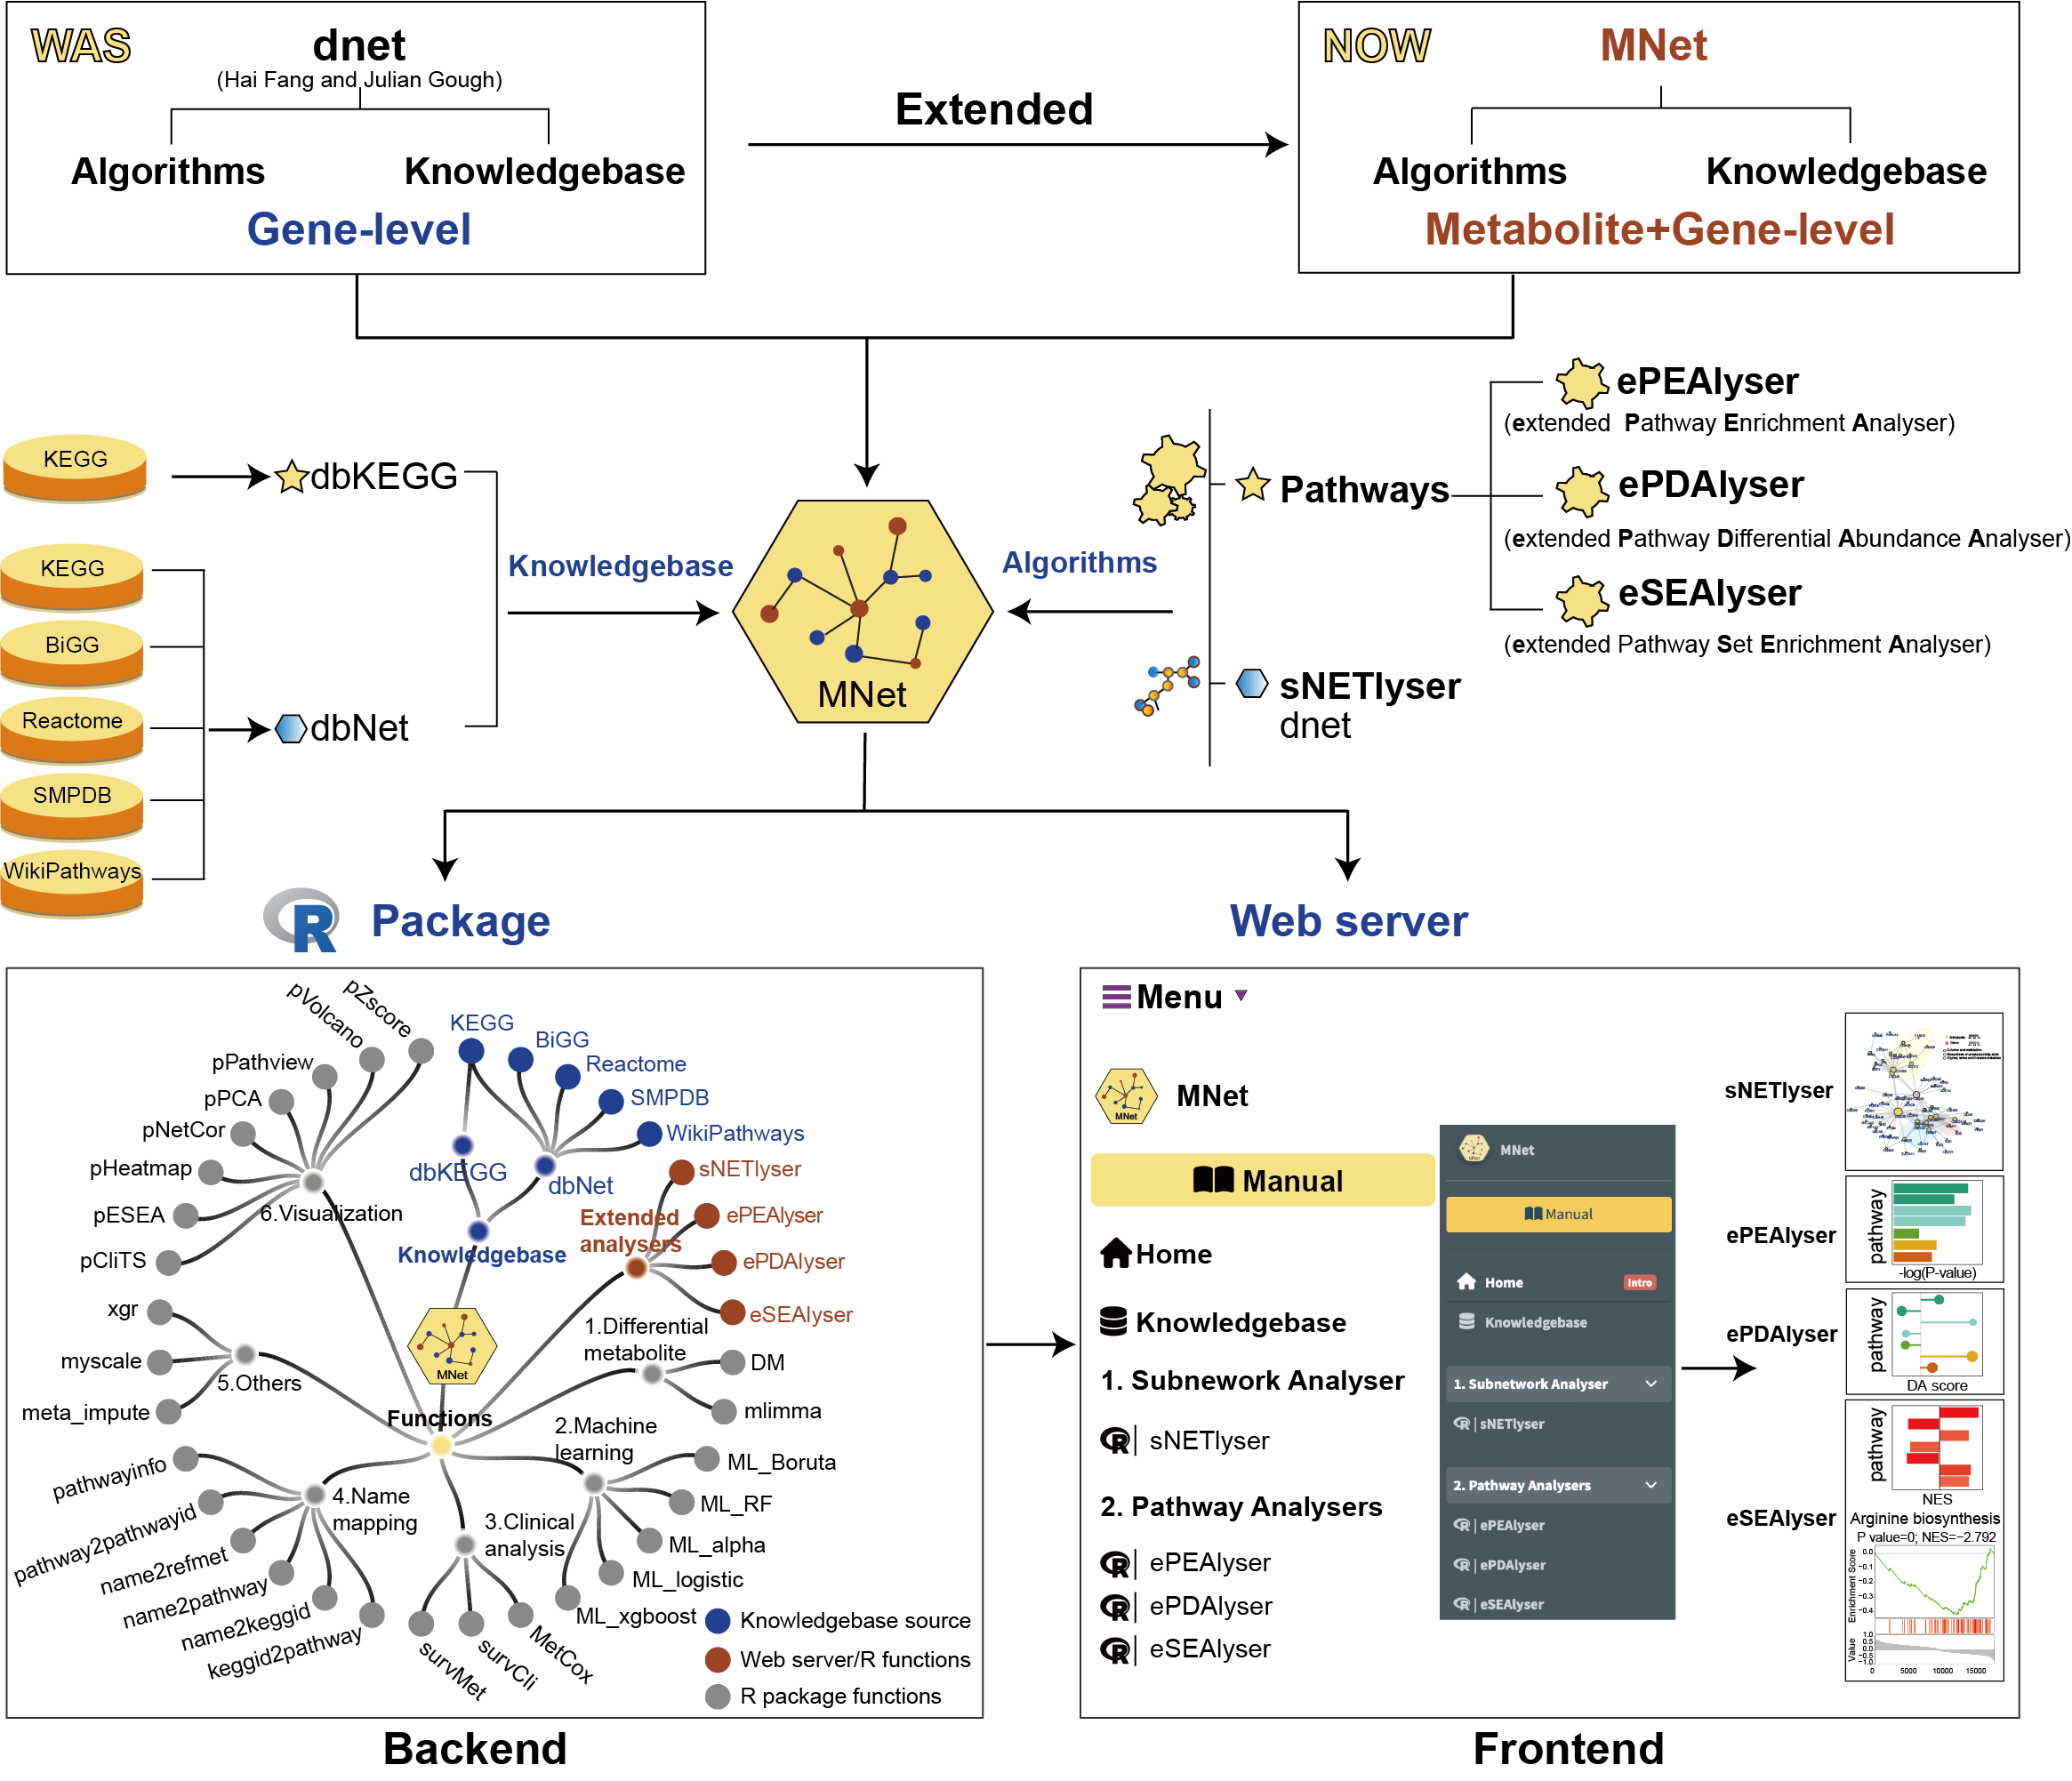
\includegraphics[width=27.58in]{figure/overview} \end{center}

\textbf{Motivation}

Advance since any previous publication (if relevant):

Integration of metabolomic and transcriptomic data is vital for pathway-centric, systems-biology understandings of disease (\href{https://doi.org/10.1093/nar/gkab1132}{Nucleic Acids Research 2022} and \href{https://doi.org/10.1038/s42003-023-05548-w}{Communications Biology 2023}). Existing pathway knowledgebases, including but not limited to BiGG (\href{https://doi.org/10.1093/nar/gkz1054}{Nucleic Acids Research 2020}), KEGG (\href{https://doi.org/10.1093/nar/gkac963}{Nucleic Acids Research 2023}), Reactome (\href{https://doi.org/10.1093/nar/gkad1025}{Nucleic Acids Research 2024}), SMPDB (\href{https://doi.org/10.1093/nar/gkt1067}{Nucleic Acids Research 2014}), and WikiPathways (\href{https://doi.org/10.1093/nar/gkad960}{Nucleic Acids Research 2024}), provide metabolic pathway information on genes and metabolites. However, these databases lack the comprehensive integration of both metabolites and genes necessary for downstream pathway and subnetwork analyses, thereby limiting the exploration of potential therapeutic targets from a metabolomic perspective.

Our well-established algorithm/tool called `dnet' and its related software(\href{https://doi.org/10.1186/s13073-014-0064-8}{Genome Medicine 2014}, \href{https://doi.org/10.1186/s13073-016-0384-y}{Genome Medicine 2016} and \href{https://doi.org/10.1038/s41588-019-0456-1}{Nature Genetics 2019}) have received nearly 400 citations over time (AS OF October 2024 according to Google Scholar). They excel at identifying core subnetwork using prior knowledge but has been limited to genomic or transcriptomic challenges, without extending its application to metabolomics. In this aspect, MNet supports pathway-centric, network-driven analyses, enabling by the compilation of the dbMNet knowledgebase, which includes dbKEGG and dbNet.

The dbKEGG facilitates KEGG metabolic pathway-based extended pathway analysis to identify dysregulated metabolic pathways involving both metabolites and genes.

The dbNet enhances metabolism-related subnetwork analysis by leveraging gene-metabolite and metabolite-metabolite information to identify subnetwork that best explain the input data.

\textbf{MNet Installation}

\begin{Shaded}
\begin{Highlighting}[]
\ControlFlowTok{if}\NormalTok{(}\SpecialCharTok{!}\FunctionTok{require}\NormalTok{(BiocManager))\{}
  \FunctionTok{install.packages}\NormalTok{(}\StringTok{"BiocManager"}\NormalTok{)}
\NormalTok{\}}

\ControlFlowTok{if}\NormalTok{ (}\SpecialCharTok{!}\FunctionTok{require}\NormalTok{(remotes)) \{}
\NormalTok{  BiocManager}\SpecialCharTok{::}\FunctionTok{install}\NormalTok{(}\StringTok{"remotes"}\NormalTok{, }\AttributeTok{dependencies=}\NormalTok{T)}
\NormalTok{\}}

\ControlFlowTok{if}\NormalTok{ (}\SpecialCharTok{!}\FunctionTok{require}\NormalTok{(devtools)) \{}
\NormalTok{  BiocManager}\SpecialCharTok{::}\FunctionTok{install}\NormalTok{(}\StringTok{"devtools"}\NormalTok{, }\AttributeTok{dependencies=}\NormalTok{T)}
\NormalTok{\}}

\NormalTok{BiocManager}\SpecialCharTok{::}\FunctionTok{install}\NormalTok{(}\StringTok{"hfang{-}bristol/dnet"}\NormalTok{, }\AttributeTok{dependencies=}\NormalTok{T)}
\NormalTok{BiocManager}\SpecialCharTok{::}\FunctionTok{install}\NormalTok{(}\StringTok{"tuantuangui/MNet"}\NormalTok{, }\AttributeTok{dependencies=}\NormalTok{T)}

\DocumentationTok{\#\# Check the package ‘MNet’ successfully installed}
\FunctionTok{library}\NormalTok{(}\AttributeTok{help=}\NormalTok{MNet)}
\end{Highlighting}
\end{Shaded}

\chapter{Metabolic Subnetwork}\label{metabolic-subnetwork}

\textbf{The metabolism-related subnetwork analysis is executed through an analyzer specifically designed to identify subnetwork based on input gene- and metabolite-level summary data.}

\section{Met-Gene Subnetwork}\label{met-gene-subnetwork}

\subsection{Interface}\label{interface}

\textbf{Procedure}

Step 1: Enter \textbf{Metabolite Data}, \textbf{GeneExp Data} and \textbf{Group Data}, respectively.

Step 2: Select \textbf{Nodes Number}.

In R network analysis, nodes number refers to the total count of nodes, representing individual elements or entities within the network.

Step 3: Select \textbf{Figure Format} and adjust \textbf{figure width, height and DPI}.

Step 4: Click the \textbf{User} panel to \textbf{view the input and output}, and finally click \textbf{Figure Download} and export the analysis results.

\begin{center}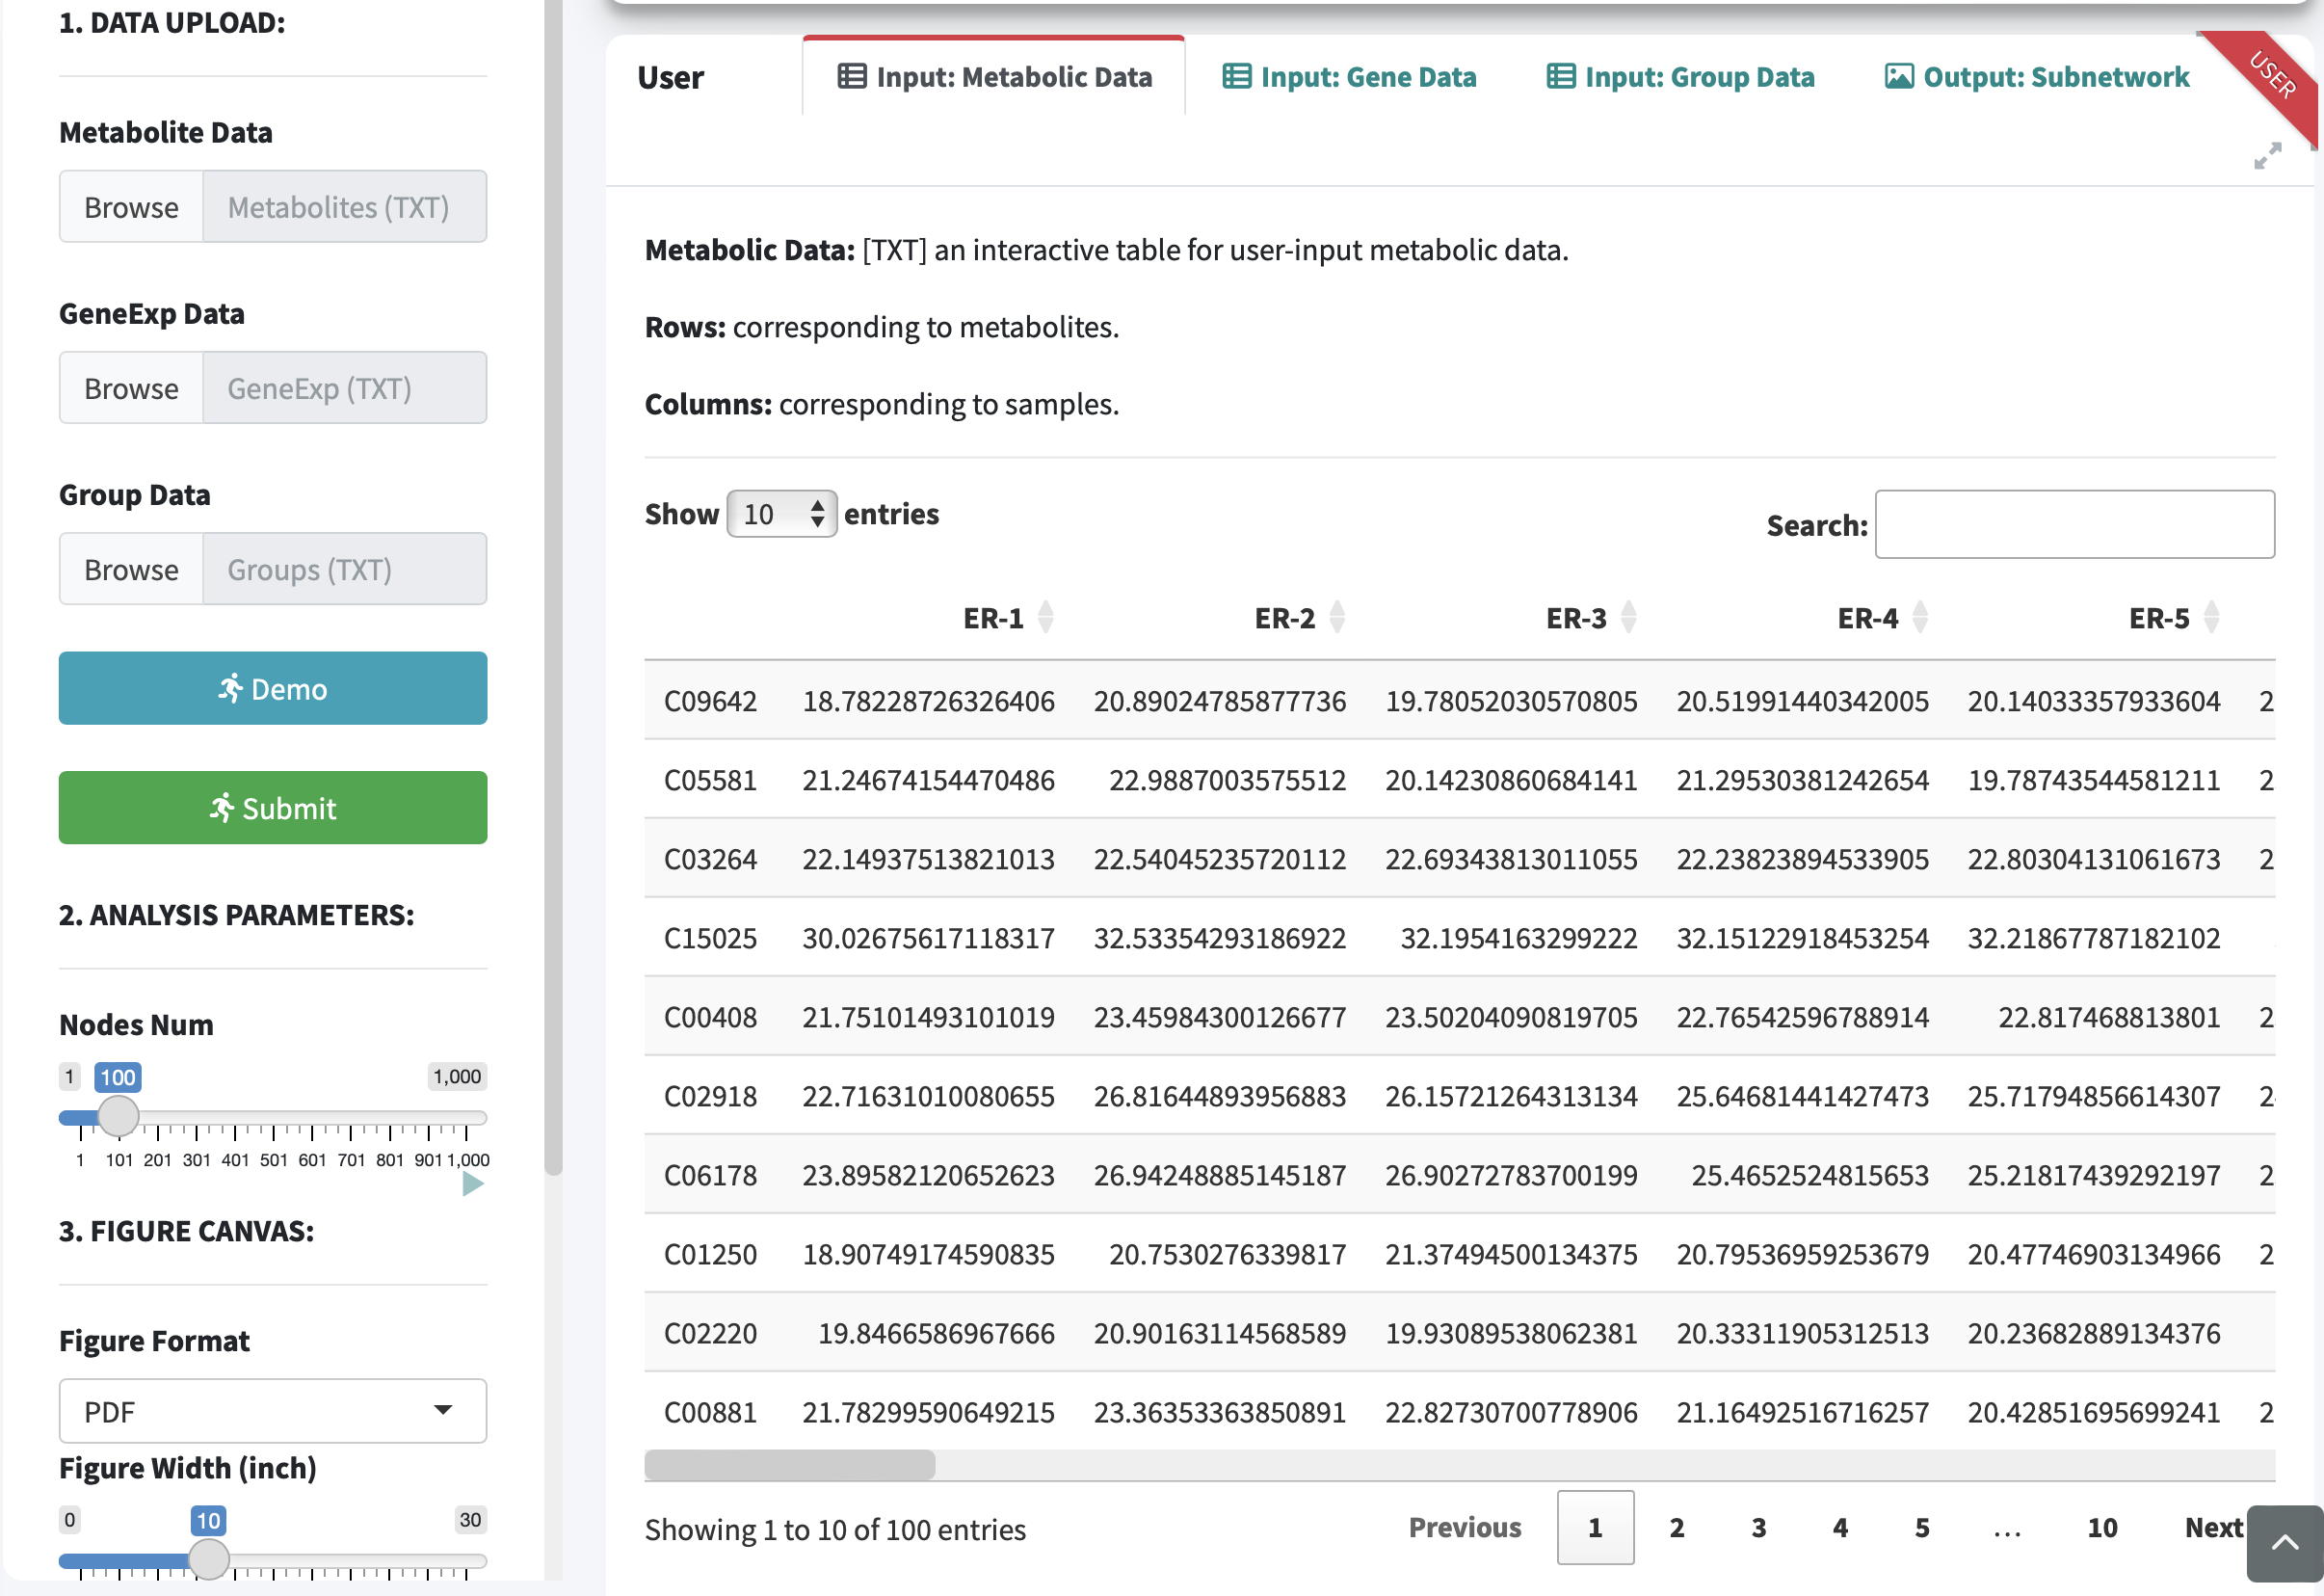
\includegraphics[width=33.5in]{figure/1.M-G} \end{center}

\textbf{Demo data}

\textbf{Expand the Demo Panel and click Metabolic Data to download demo data}, which comprises an integrated analysis of metabolomic and transcriptomic profiles in triple-negative breast cancer.

\textbf{Metabolite Data}: an interactive table for user-input metabolic data with rows corresponding to metabolites and columns corresponding to samples.

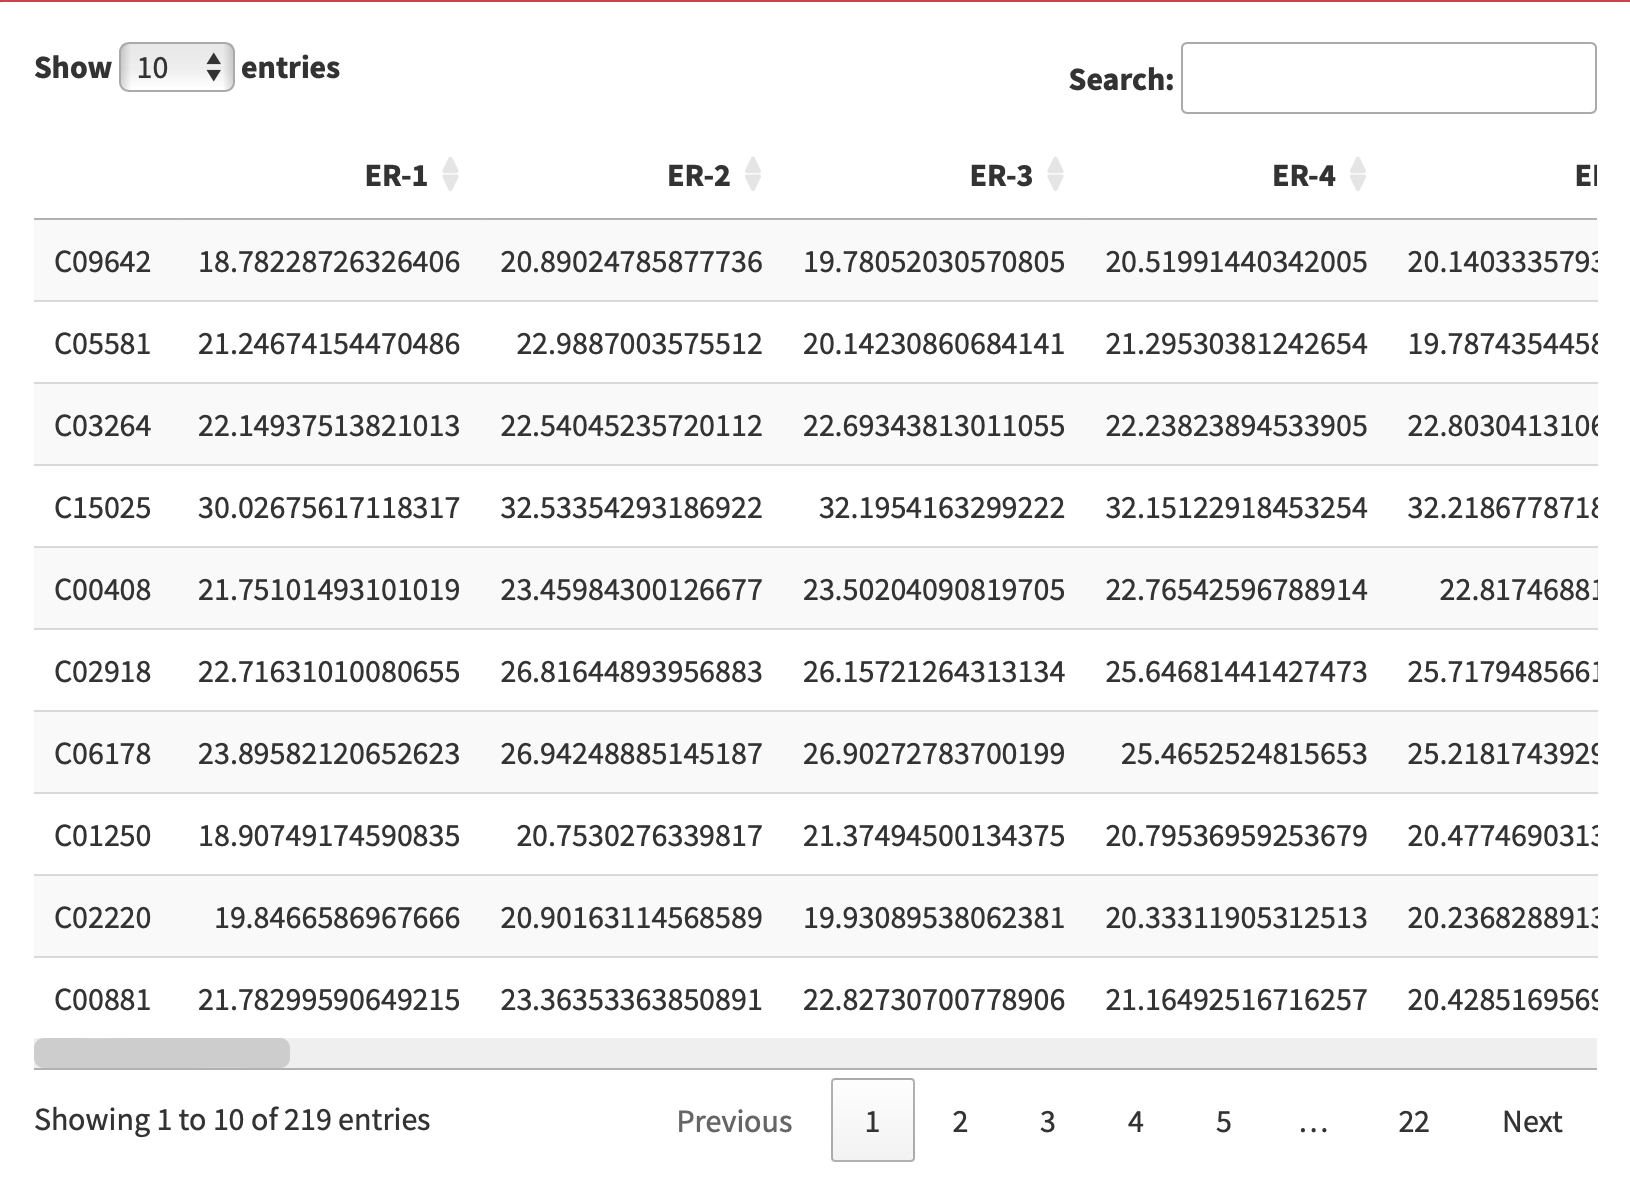
\includegraphics[width=22.64in]{figure/Metabolite}

\textbf{GeneExp Data}: an interactive table for user-input metabolic data with rows corresponding to genes and columns correspond to the samples.

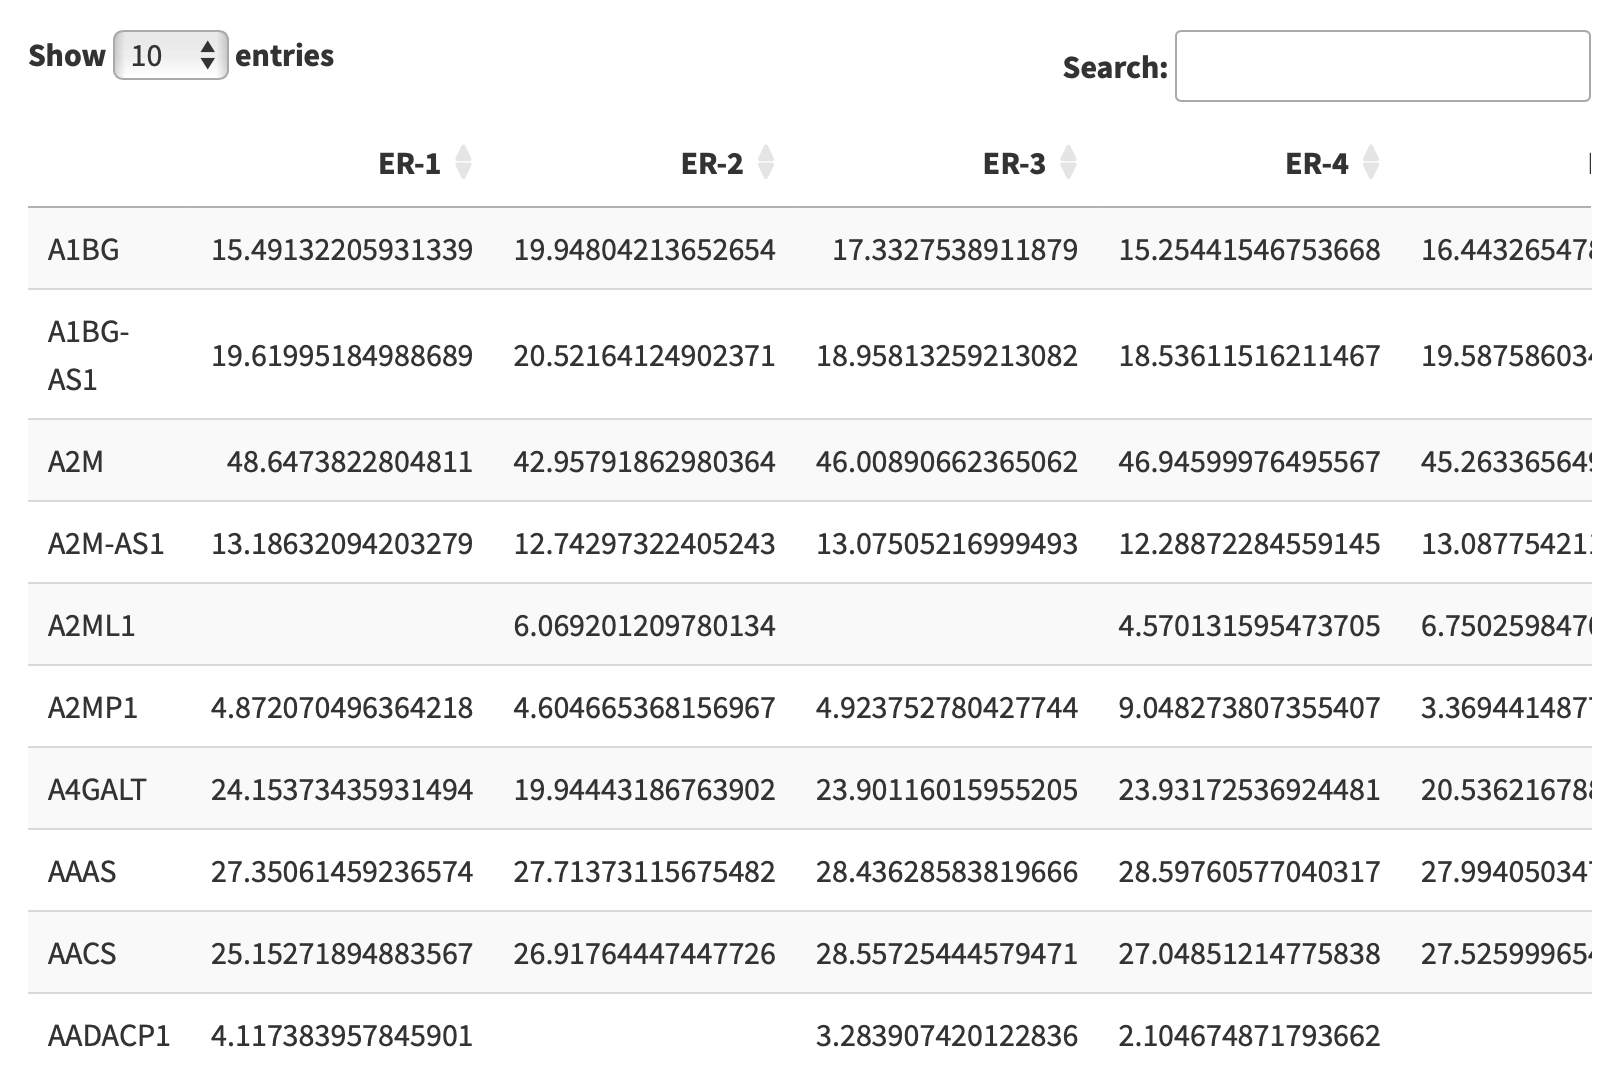
\includegraphics[width=22.42in]{figure/GeneExp}

\textbf{Group Data}: Group information.

\begin{flushleft}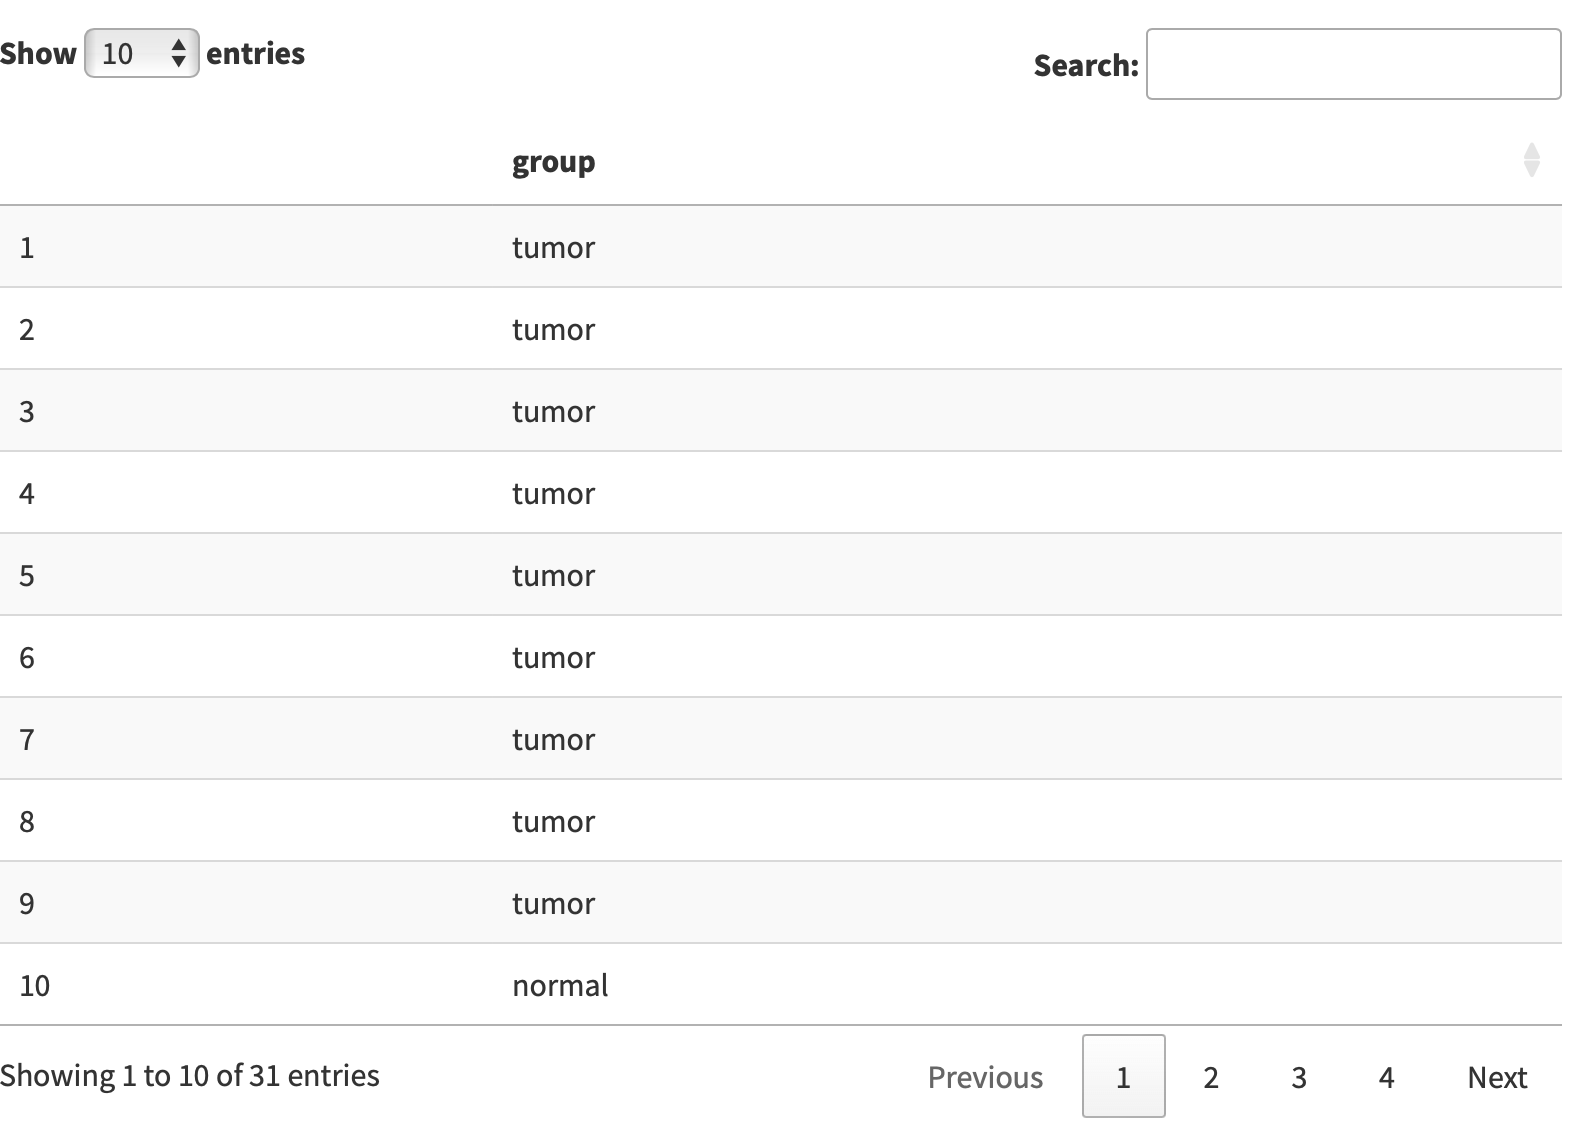
\includegraphics[width=21.83in]{figure/GroupInfo} \end{flushleft}

\subsection{Results}\label{results}

By utilising the dbNet knowledgebase and employing the dnet algorithm, MNet analyses a list of genes and metabolites along with their significance information, allowing a graphical display of the metabolism-related subnetwork that contains both genes and metabolites.

\begin{center}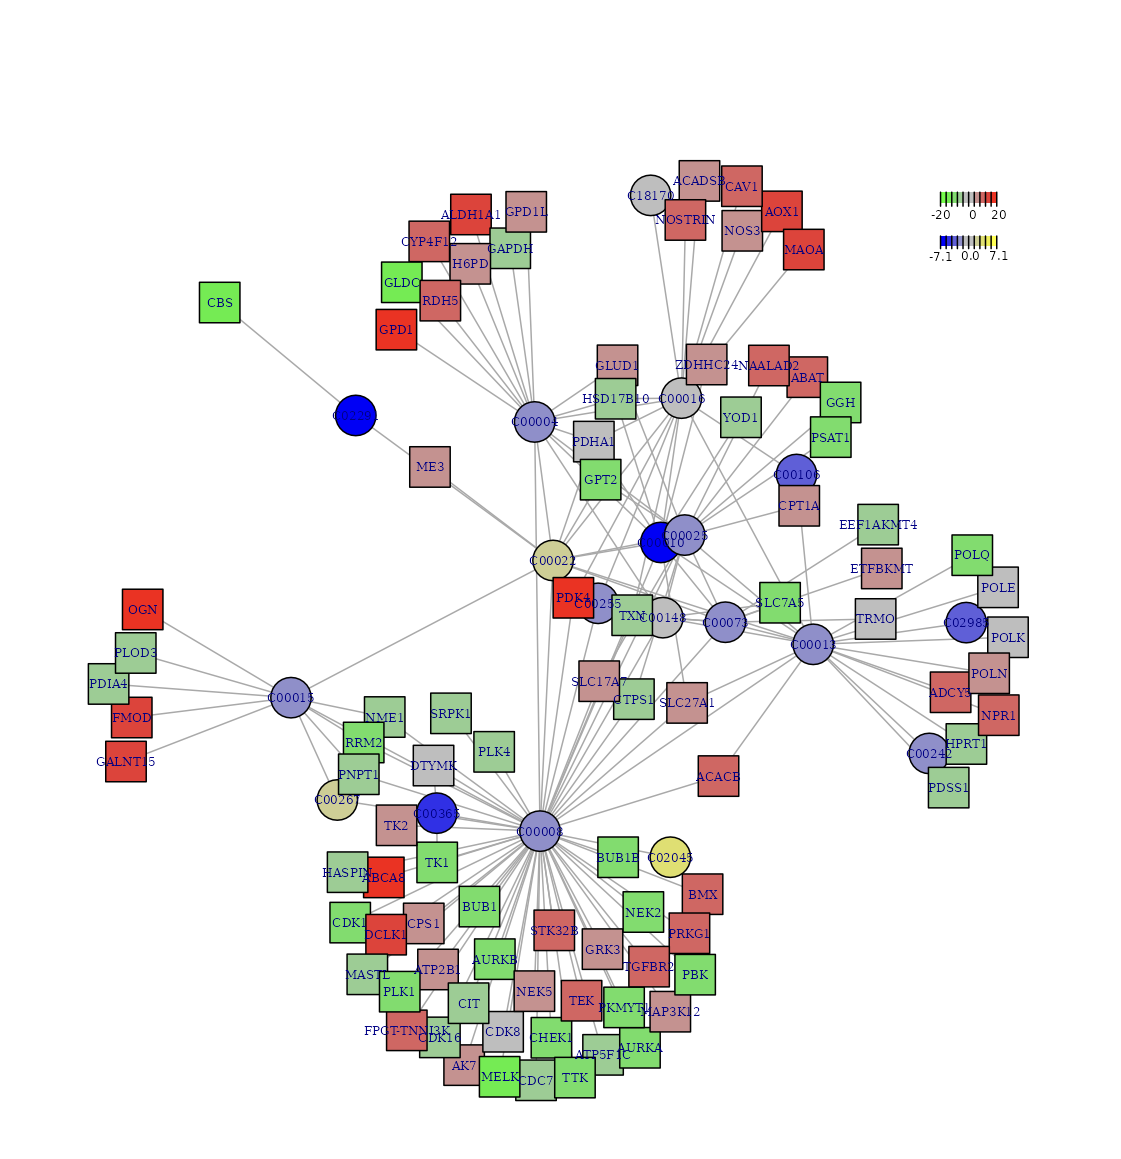
\includegraphics[width=15.57in]{figure/subnetwork} \end{center}

Figure 1. Visualization of the identified optimal subnetwork that best explains the biological processes comparing two groups. The colors represent the logFC (logarithm of fold change) of genes, with red and green indicating different expression levels, while yellow and blue represent the logFC of metabolites, indicating varying levels.

\chapter{Extended Pathway Analyses}\label{extended-pathway-analyses}

\section{ePEA}\label{epea}

Extended pathway enrichment analysis

\subsection{Interface}\label{interface-1}

\textbf{Procedure}

Step 1: Enter \textbf{Metabolite Data}, \textbf{GeneExp Data} and \textbf{Group Data}, respectively.

Step 2: Select \textbf{Log(FoldChange), Padjust Cutoff and Pathway Pcutoff}, respectively.

\textbf{Fold change}: Identifies key metabolites with significant expression shifts between conditions, revealing potential metabolic alterations and pathway involvement in biological processes.

\textbf{Padjust Cutoff}: Helps filter significant results by controlling for false positives, ensuring that only statistically robust pathways are identified for further investigation.

\textbf{Pathway Pcutoff}: Sets a significance threshold, helping to identify pathways with meaningful changes while reducing the likelihood of false-positive findings.

Step 3: Select \textbf{Figure Format} and adjust \textbf{figure width, height and DPI}.

Step 4: Click the \textbf{User} panel to \textbf{view the input and output}, and finally click \textbf{Figure Download} and export the analysis results.

\begin{center}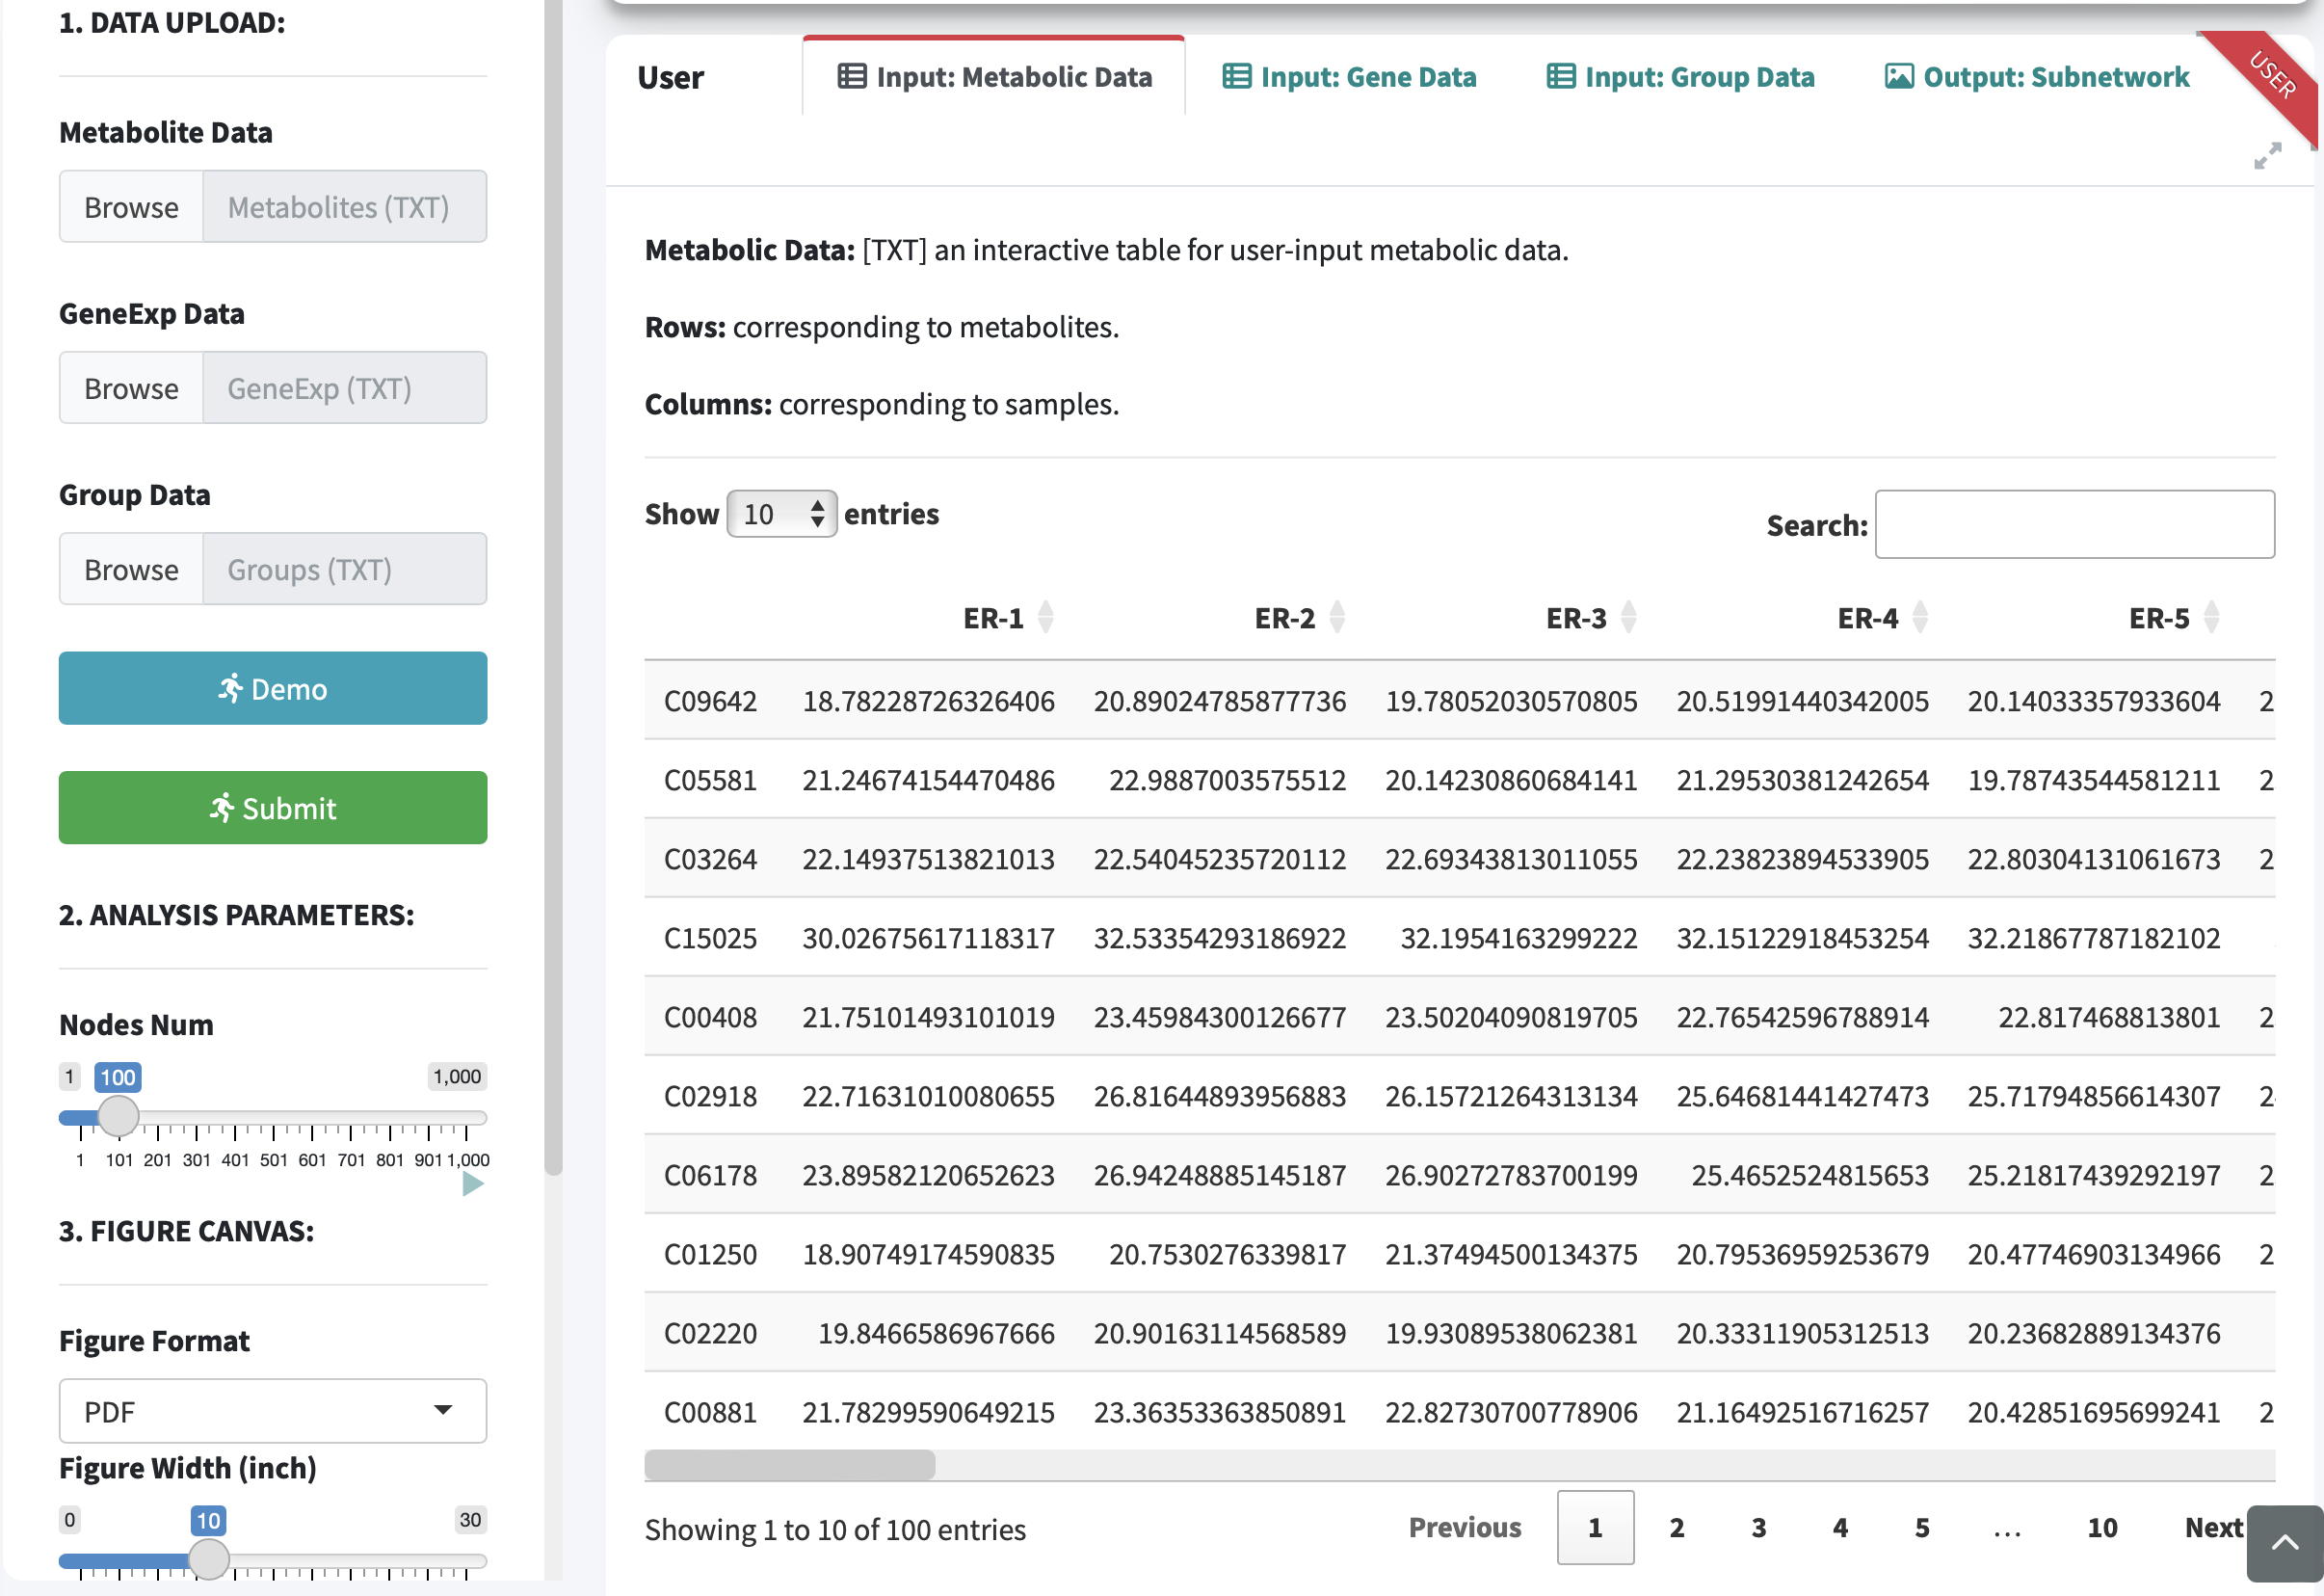
\includegraphics[width=33.5in]{figure/1.M-G} \end{center}

\textbf{Demo data}

\textbf{Expand the Demo Panel and click Metabolic Data to download demo data}, which comprises an integrated analysis of metabolomic and transcriptomic profiles in triple-negative breast cancer.

\textbf{Metabolite Data}: an interactive table for user-input metabolic data with rows corresponding to metabolites and columns corresponding to samples.

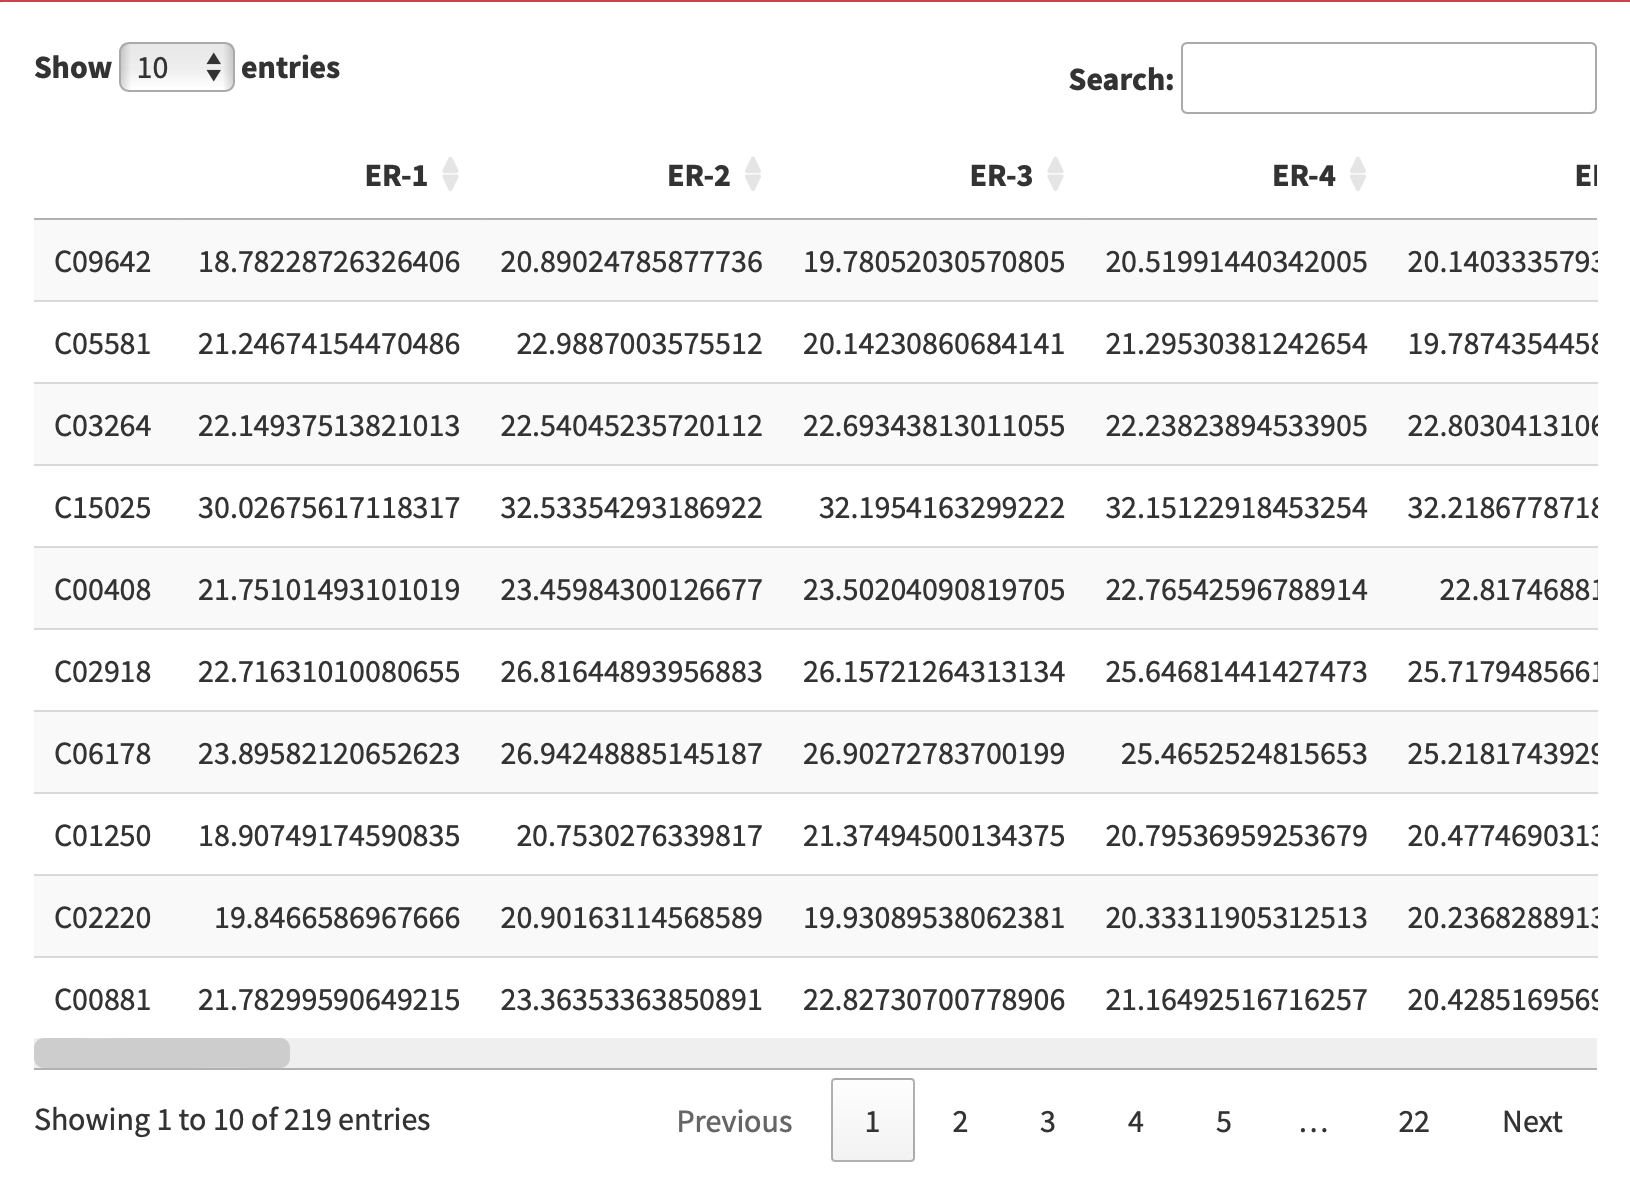
\includegraphics[width=22.64in]{figure/Metabolite}

\textbf{GeneExp Data}: an interactive table for user-input metabolic data with rows corresponding to genes and columns correspond to the samples.

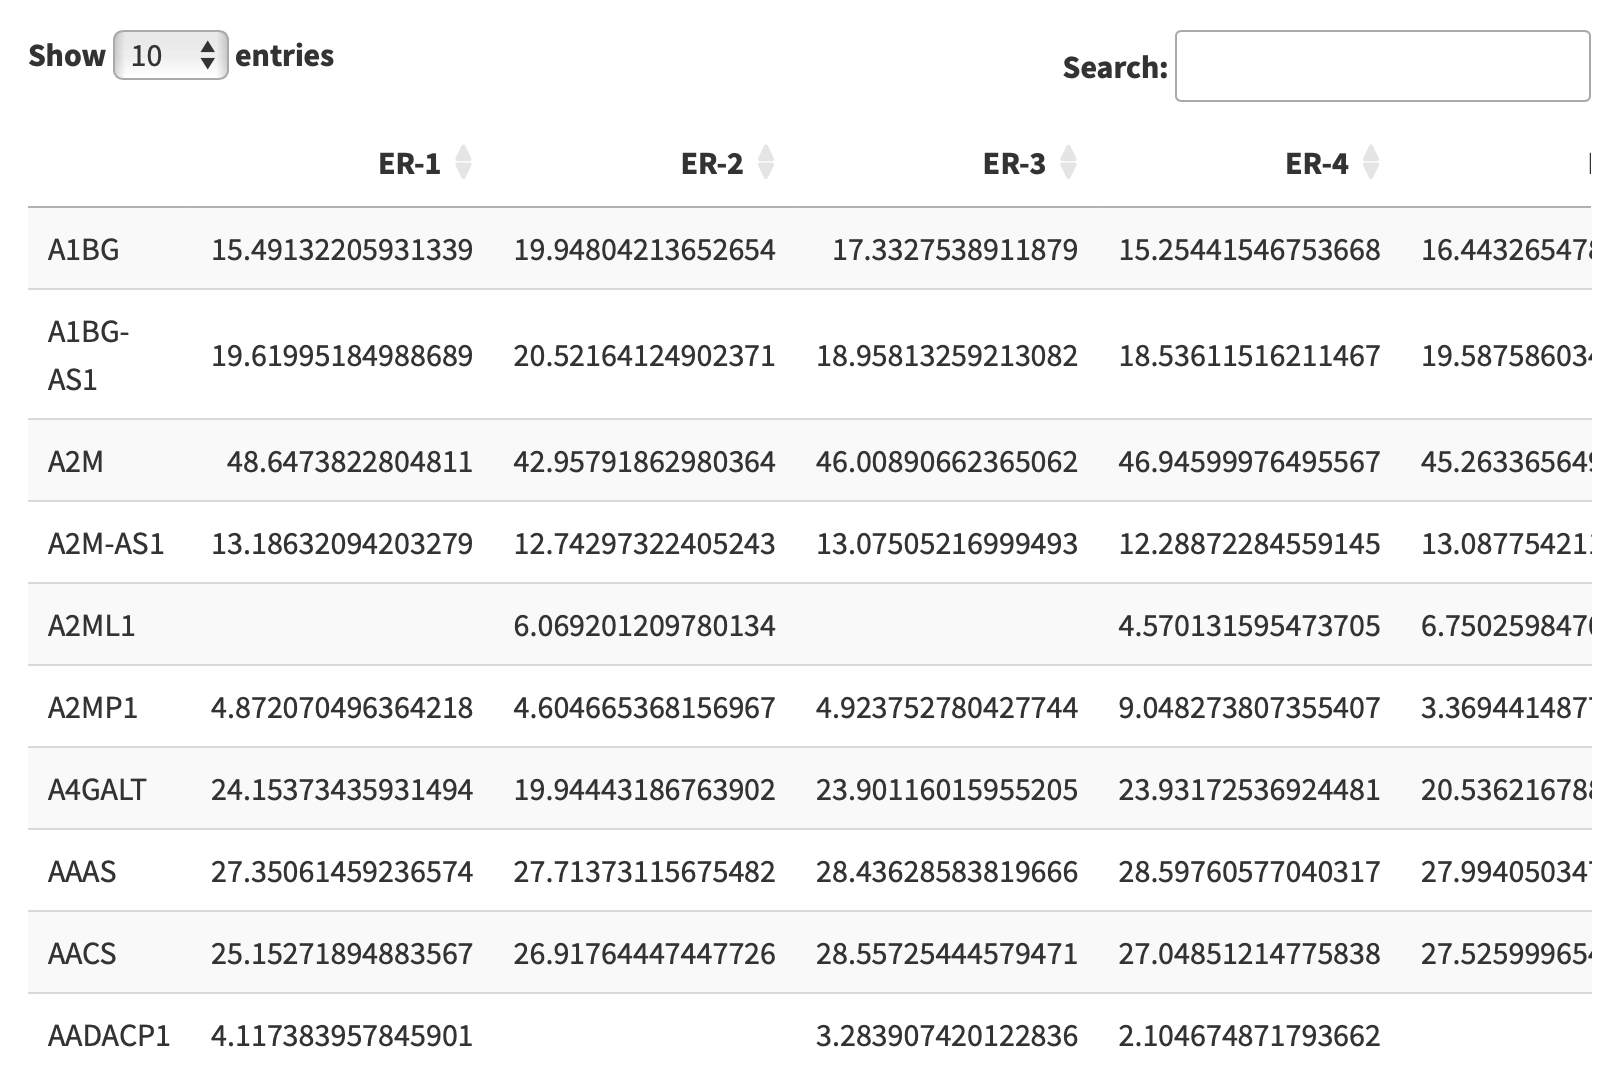
\includegraphics[width=22.42in]{figure/GeneExp}

\textbf{Group Data}: Group information.

\begin{flushleft}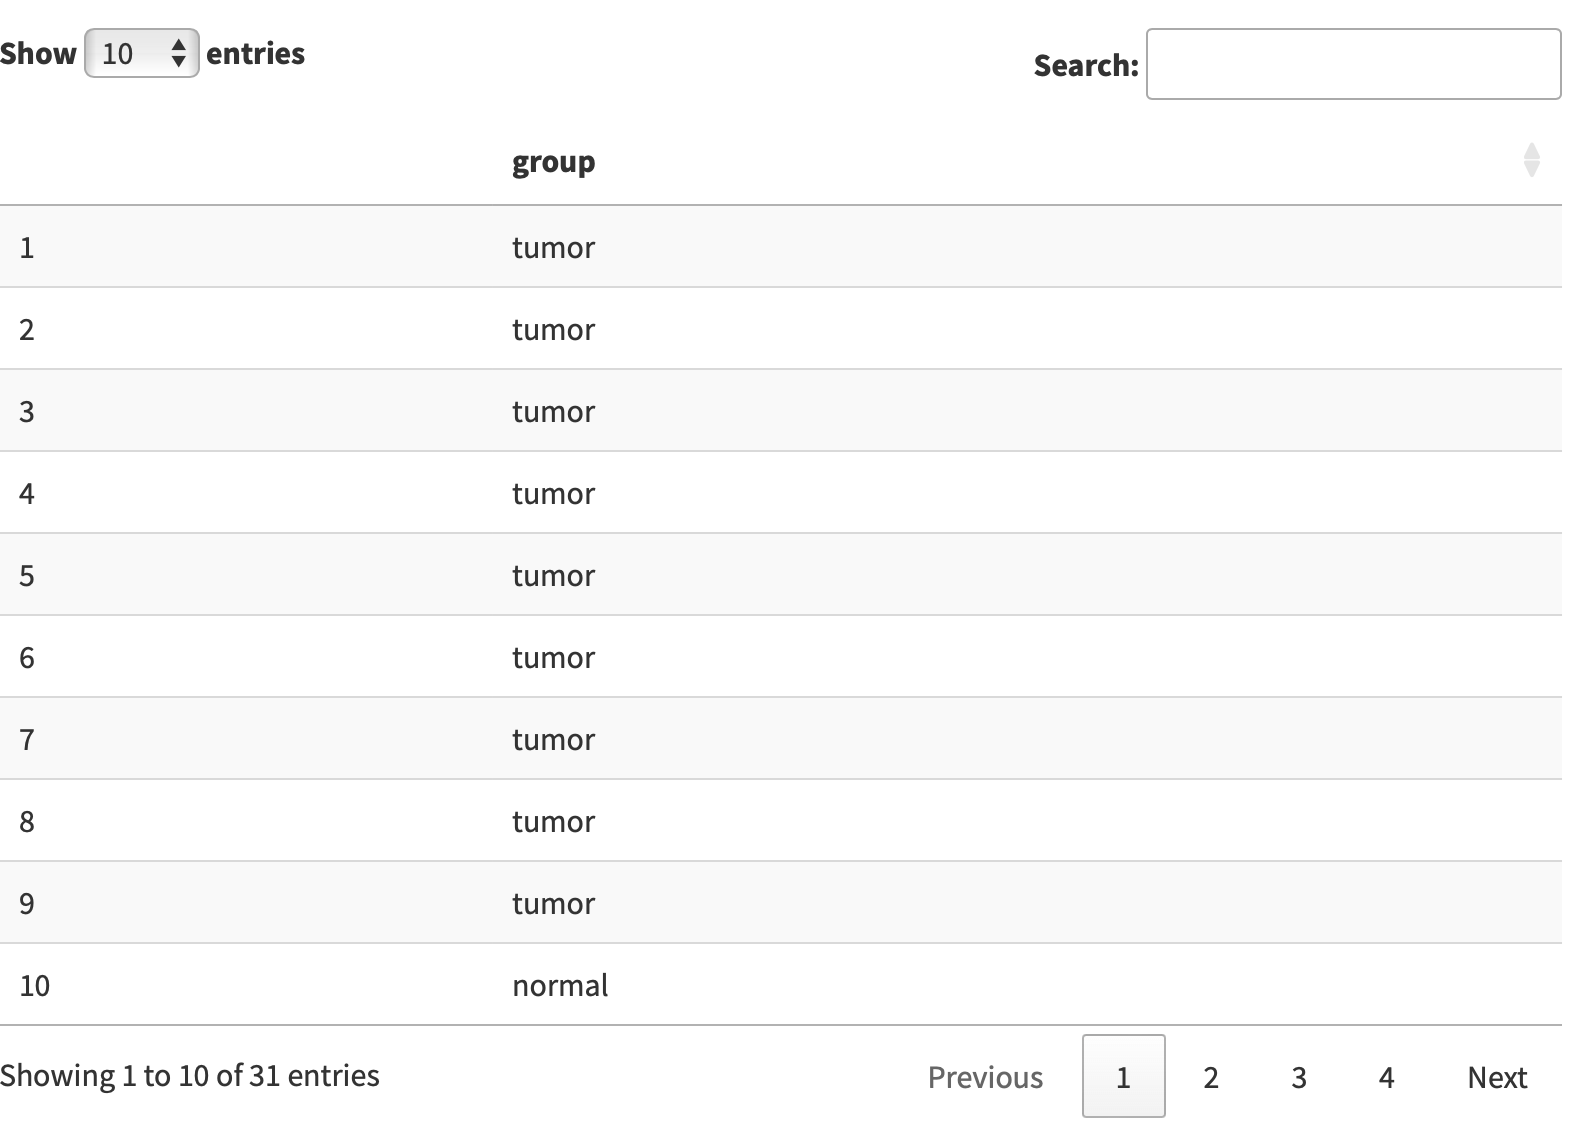
\includegraphics[width=21.83in]{figure/GroupInfo} \end{flushleft}

\subsection{Results}\label{results-1}

\begin{center}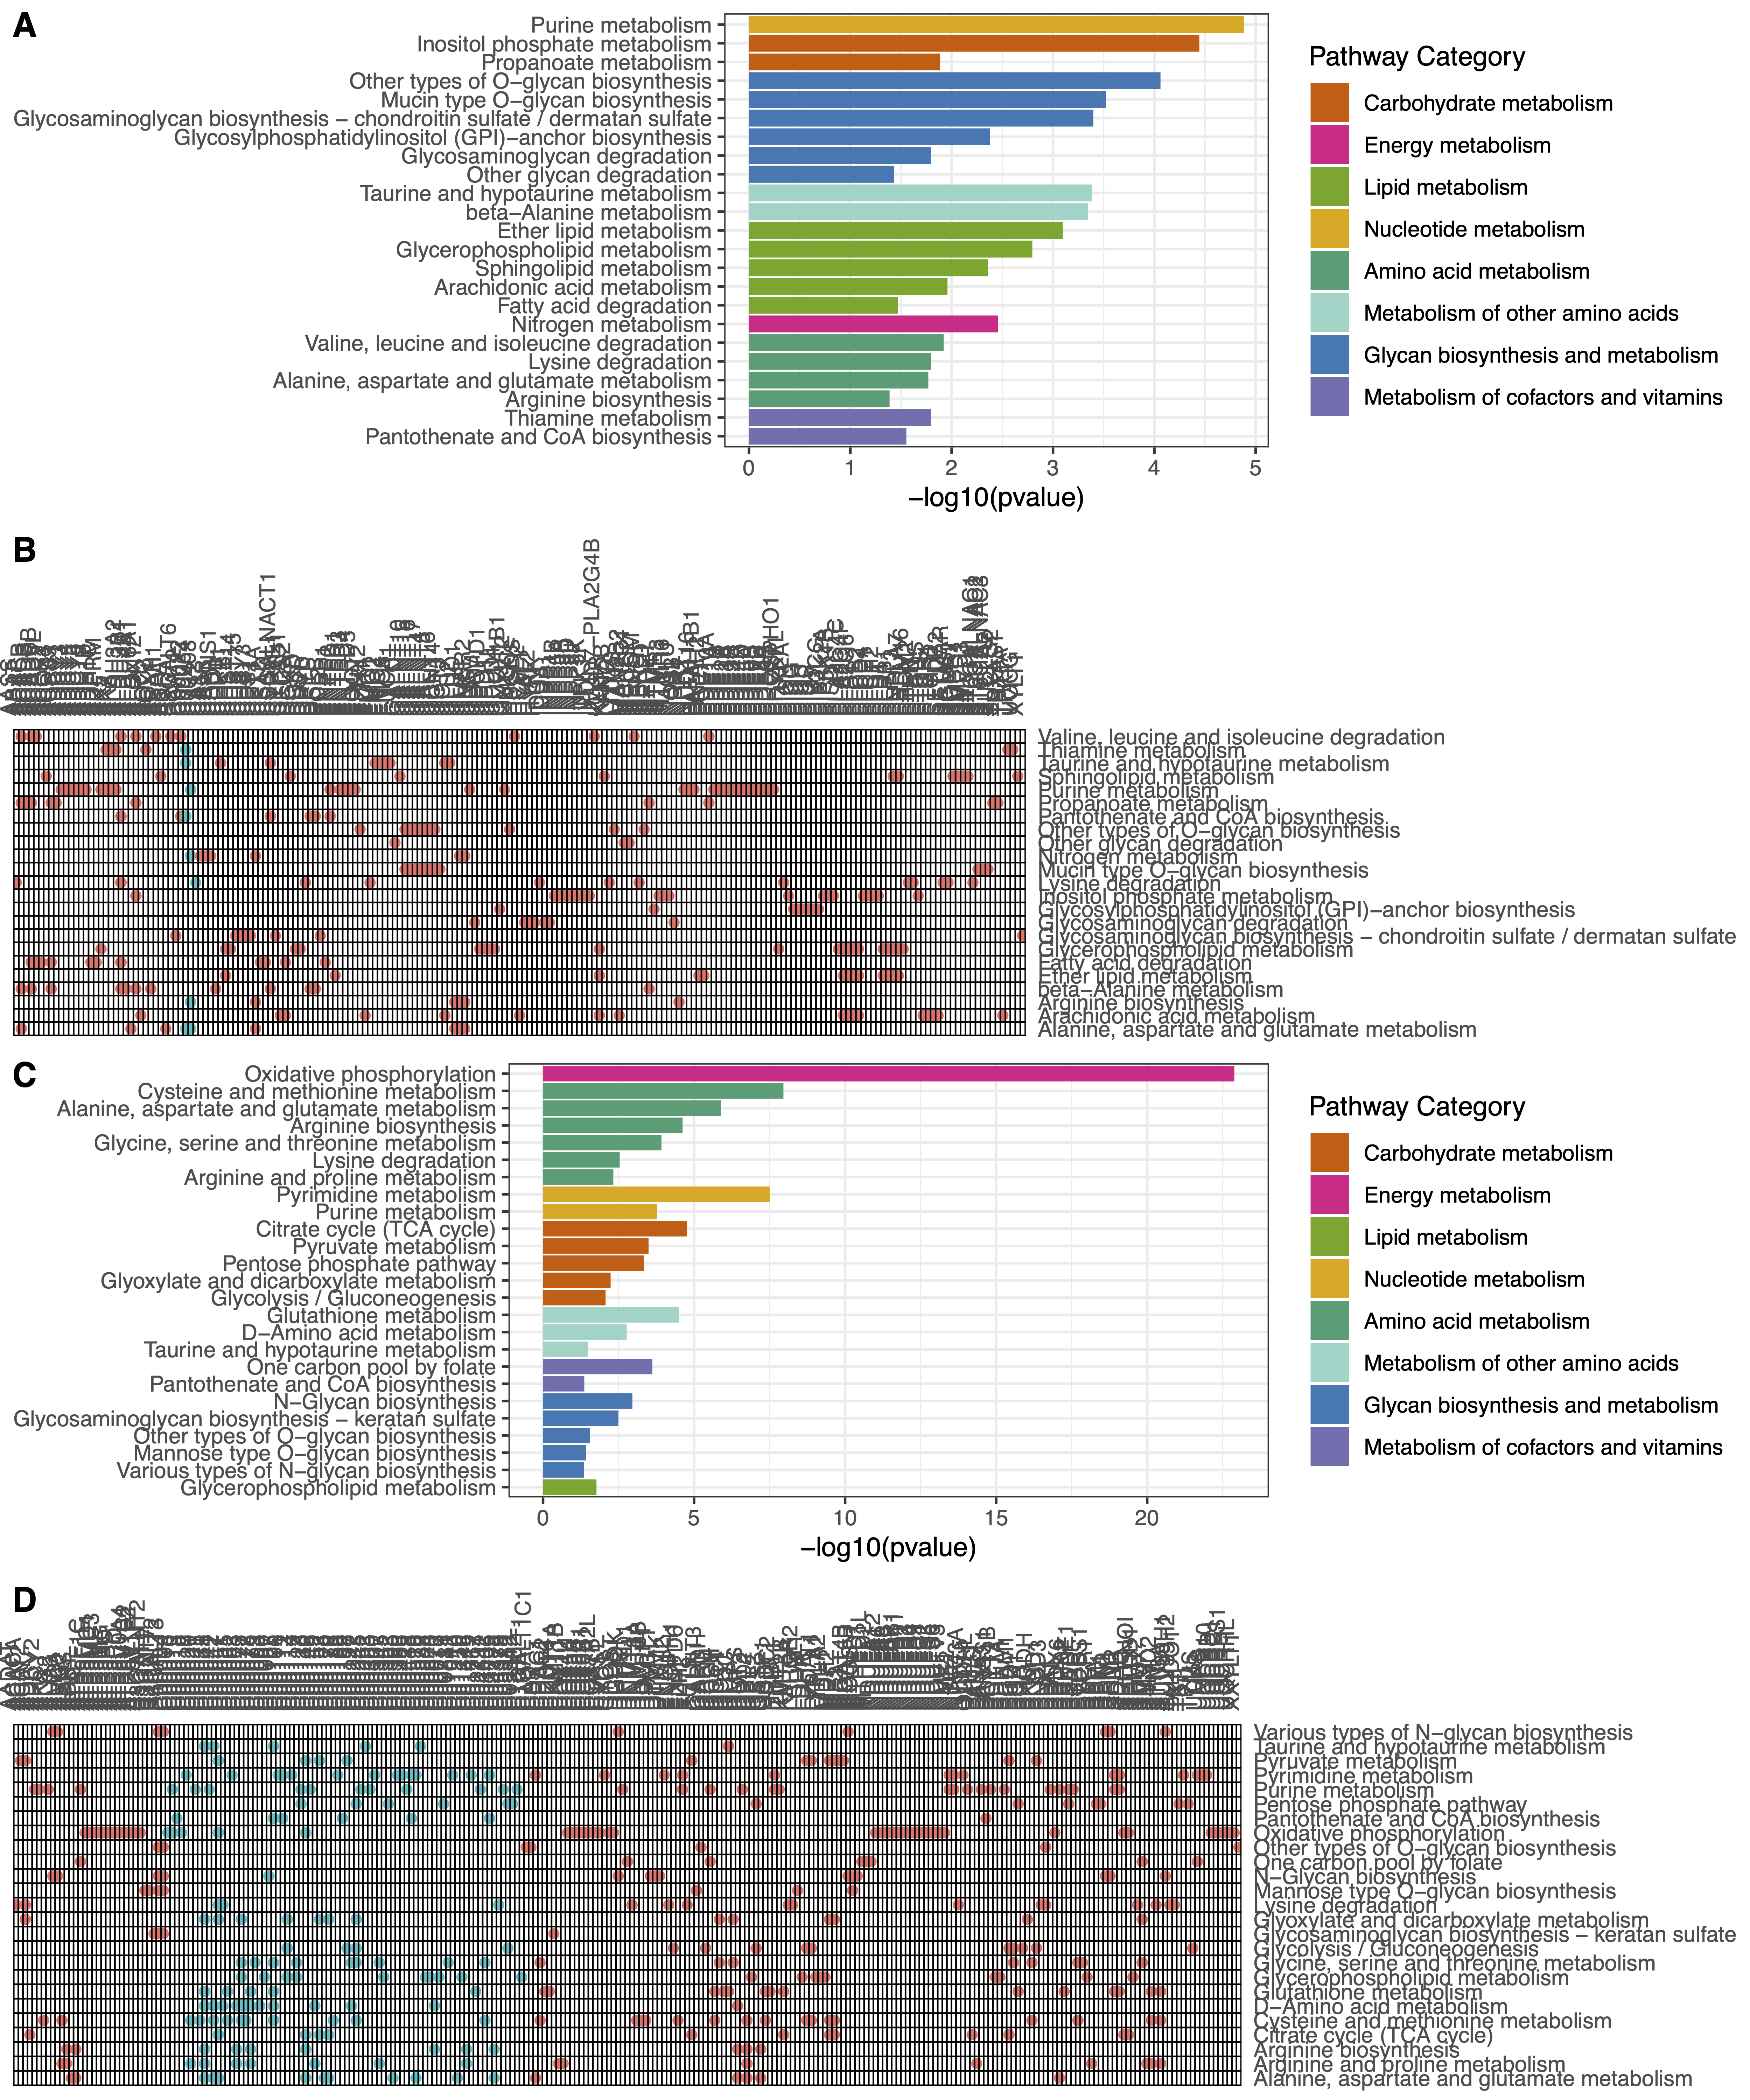
\includegraphics[width=70.83in]{figure/2.ePEA} \end{center}

Figure 1. Extended pathway enrichment analysis. (A) Barplot of up-regulated metabolic pathways corresponding to metabolites and genes. (B) Dotplot of up-regulated metabolic pathways corresponding to metabolites and genes. (C) Barplot of down-regulated metabolic pathways corresponding to metabolites and genes. (D) Dotplot of down-regulated metabolic pathways corresponding to metabolites and genes.

\section{ePDA}\label{epda}

Extended pathway differential abundance (ePDA) score

\subsection{Interface}\label{interface-2}

\textbf{Procedure}

Step 1: Enter \textbf{Metabolite Data}, \textbf{GeneExp Data} and \textbf{Group Data}, respectively.

Step 2: Select \textbf{Log(FoldChange), Padjust Cutoff and Pathway Pcutoff}, respectively.

\textbf{Fold change}: Identifies key metabolites with significant expression shifts between conditions, revealing potential metabolic alterations and pathway involvement in biological processes.

\textbf{Padjust Cutoff}: Helps filter significant results by controlling for false positives, ensuring that only statistically robust pathways are identified for further investigation.

\textbf{Pathway Pcutoff}: Sets a significance threshold, helping to identify pathways with meaningful changes while reducing the likelihood of false-positive findings.

Step 3: Select \textbf{Figure Format} and adjust \textbf{figure width, height and DPI}.

Step 4: Click the \textbf{User} panel to \textbf{view the input and output}, and finally click \textbf{Figure Download} and export the analysis results.

\begin{center}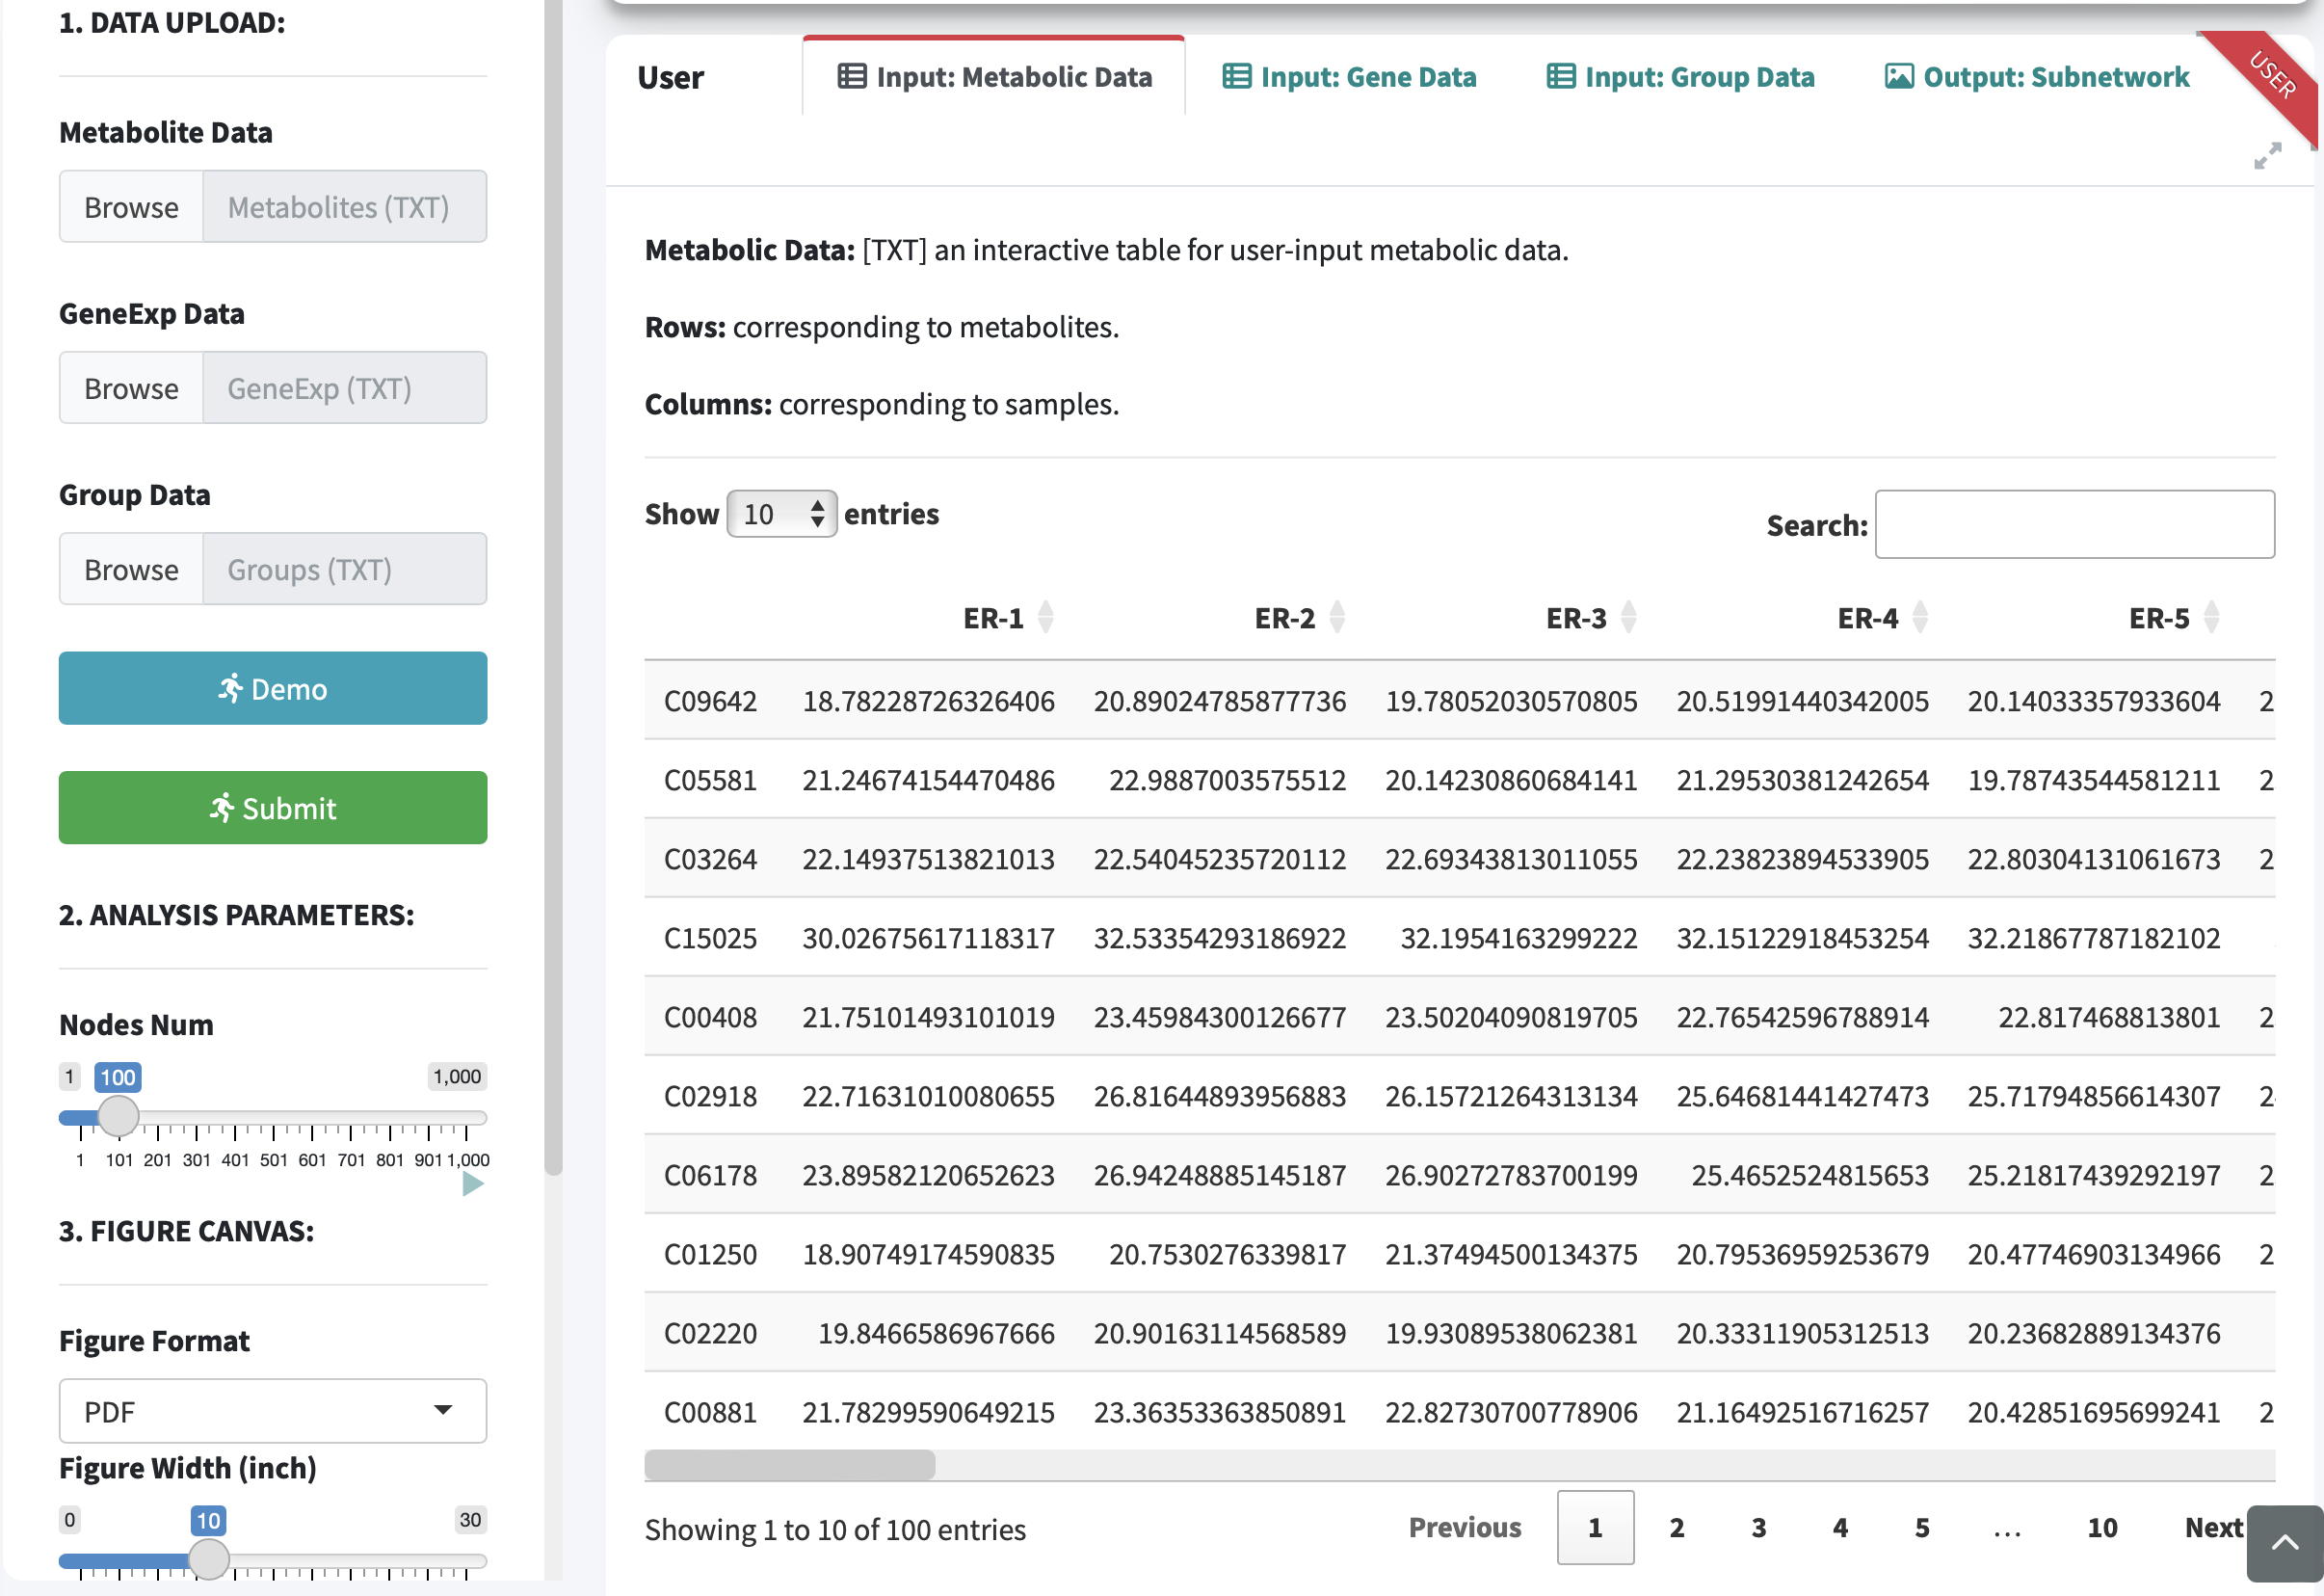
\includegraphics[width=33.5in]{figure/1.M-G} \end{center}

\textbf{Demo data}

\textbf{Expand the Demo Panel and click Metabolic Data to download demo data}, which comprises an integrated analysis of metabolomic and transcriptomic profiles in triple-negative breast cancer.

\textbf{Metabolite Data}: an interactive table for user-input metabolic data with rows corresponding to metabolites and columns corresponding to samples.

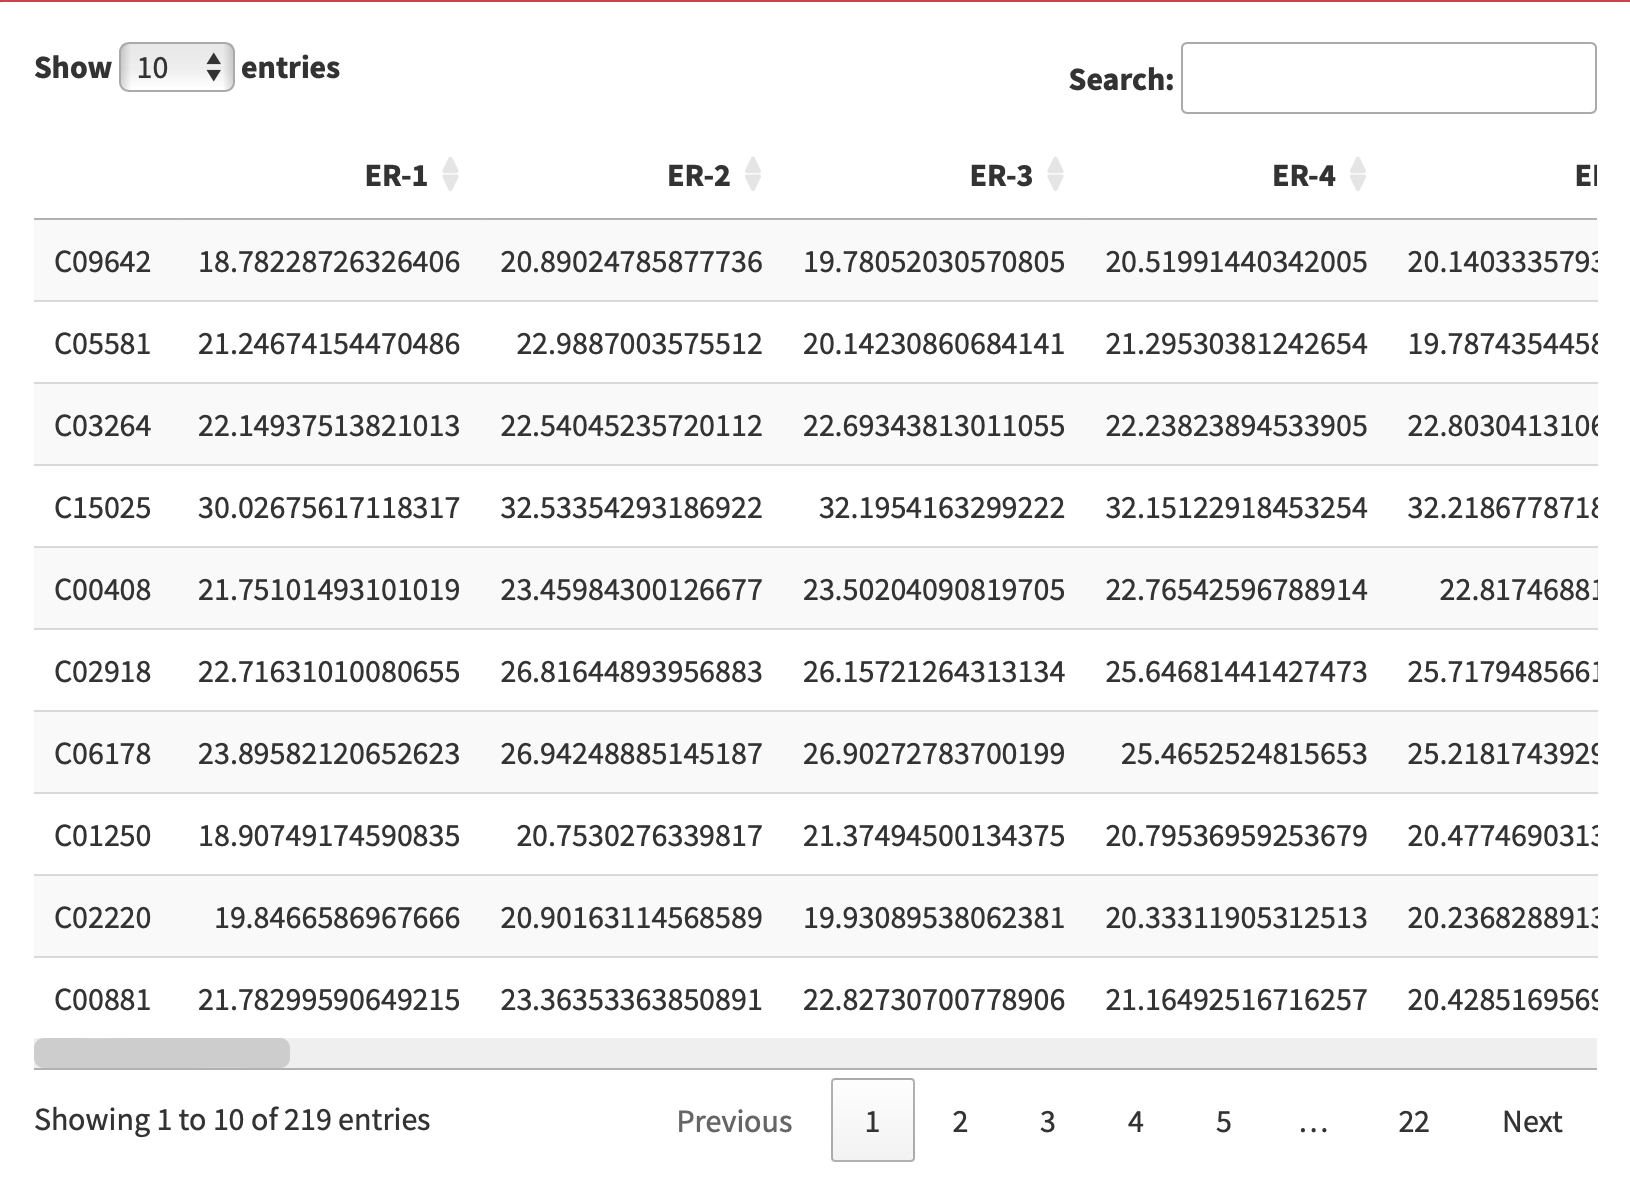
\includegraphics[width=22.64in]{figure/Metabolite}

\textbf{GeneExp Data}: an interactive table for user-input metabolic data with rows corresponding to genes and columns correspond to the samples.

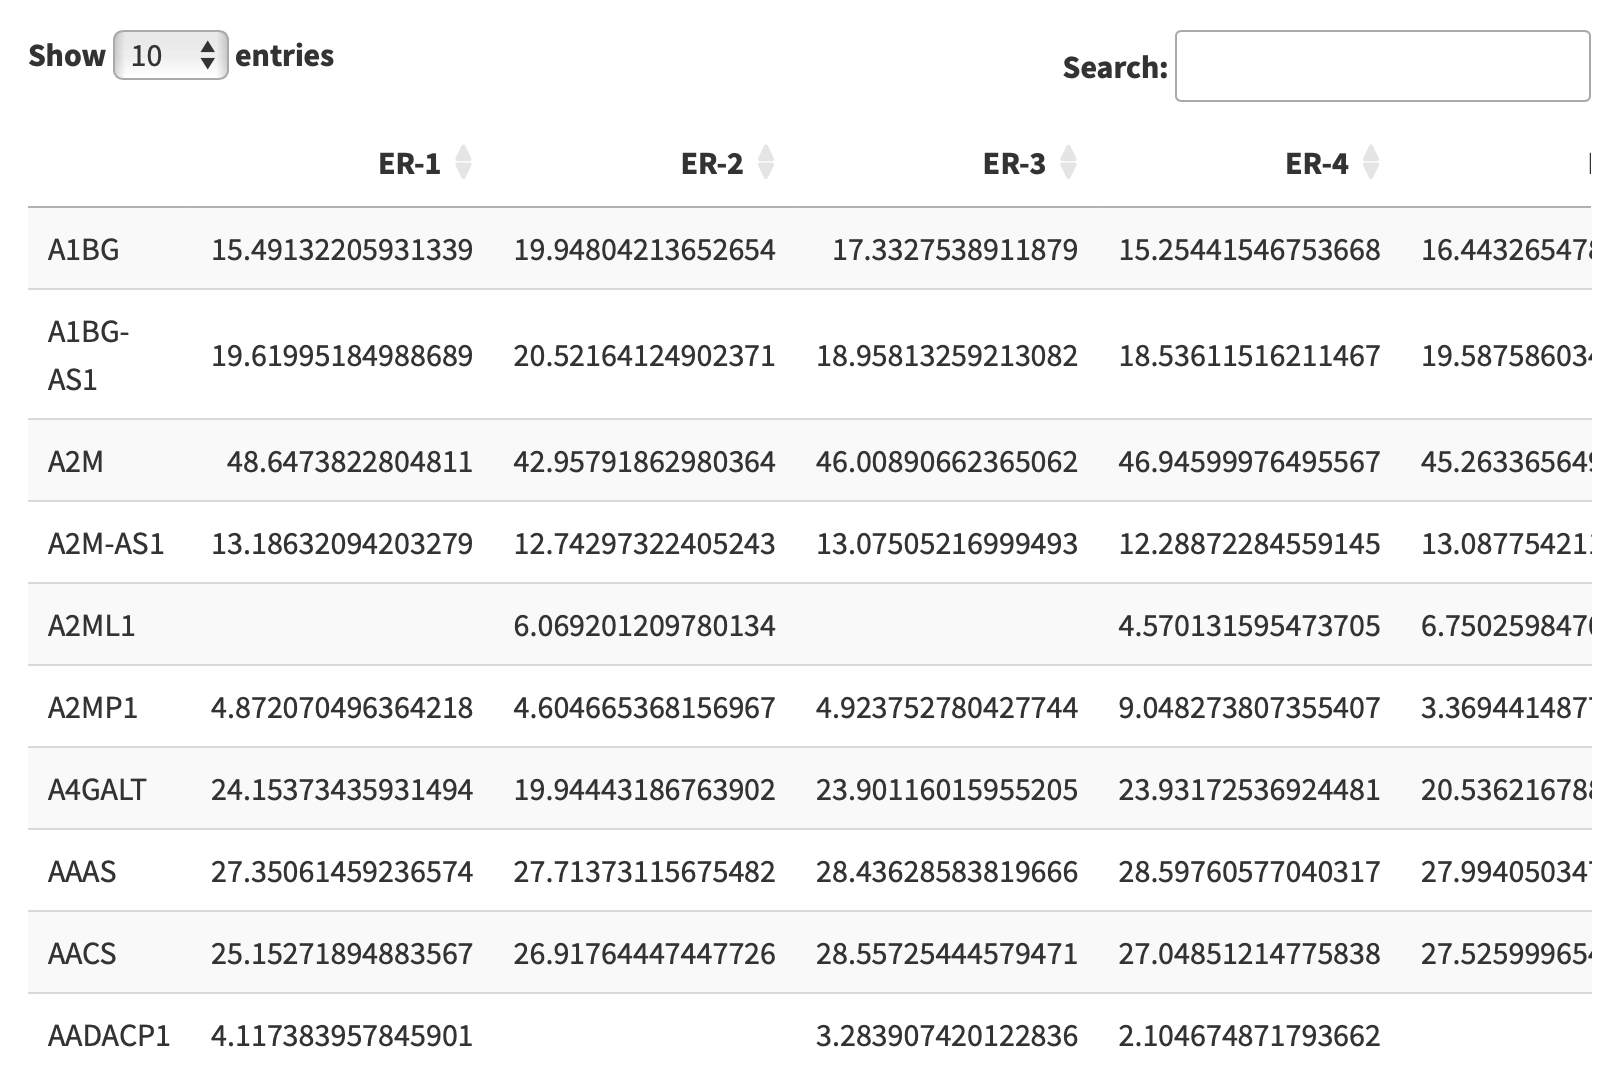
\includegraphics[width=22.42in]{figure/GeneExp}

\textbf{Group Data}: Group information.

\begin{flushleft}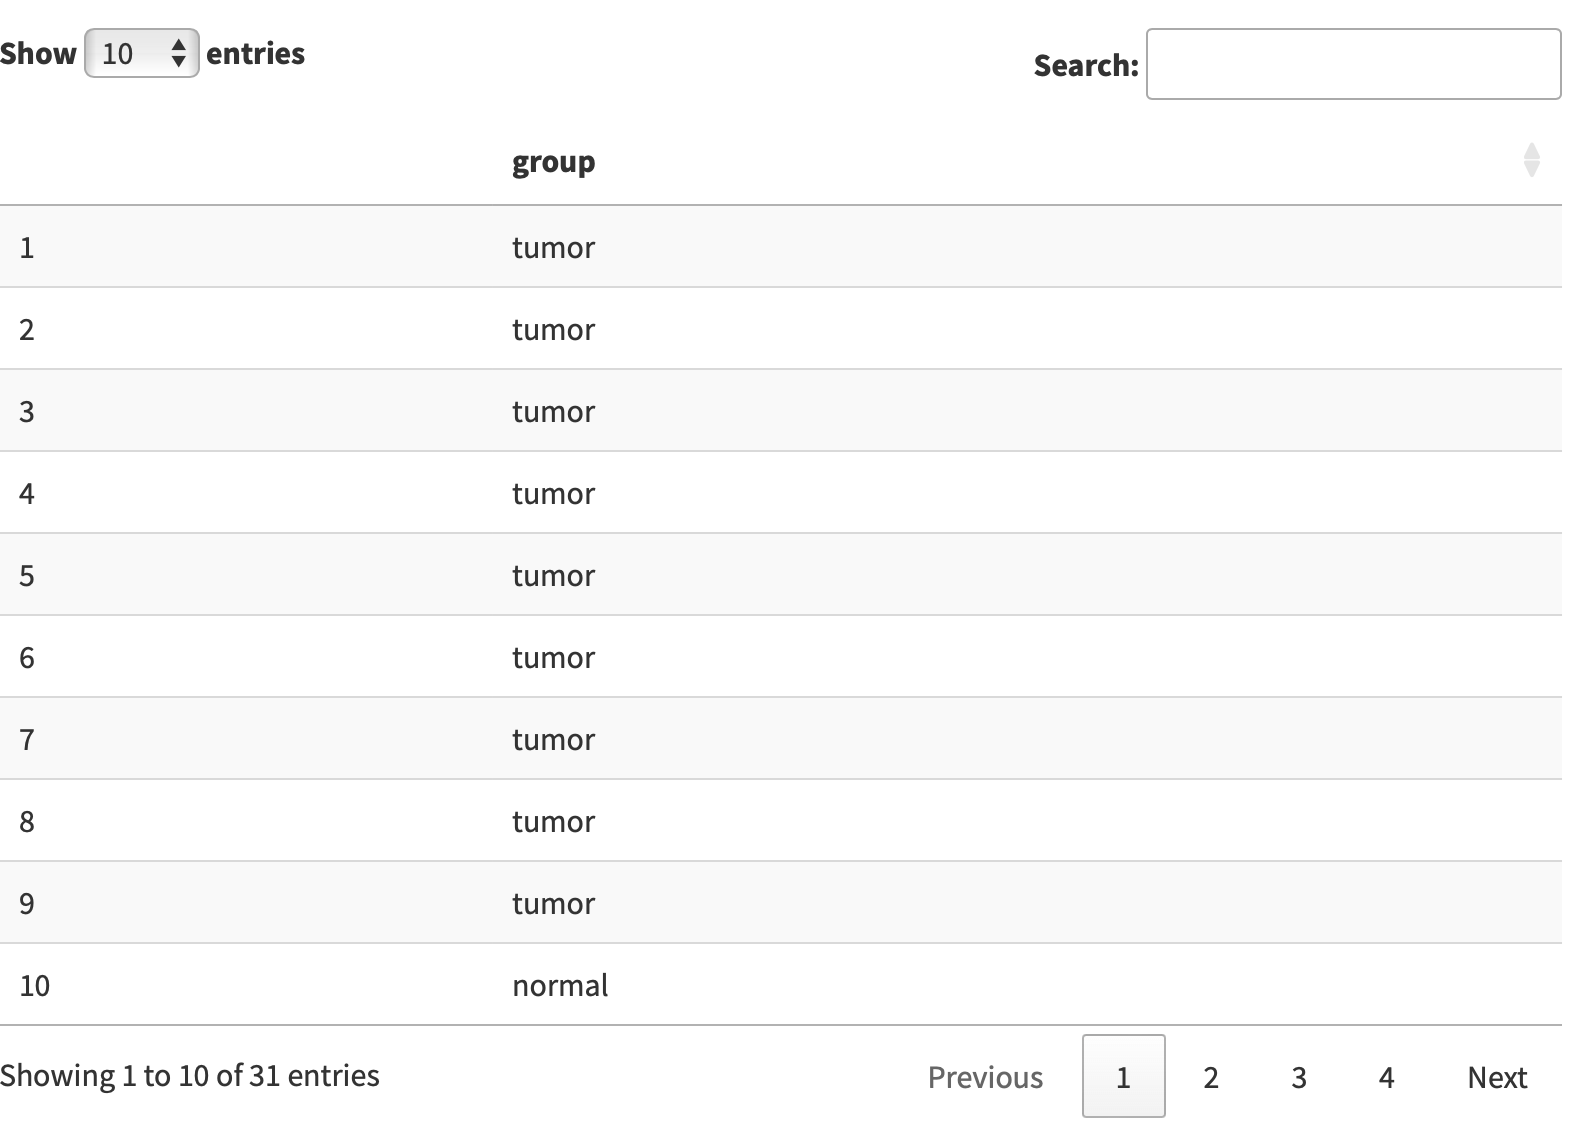
\includegraphics[width=21.83in]{figure/GroupInfo} \end{flushleft}

\subsection{Results}\label{results-2}

\begin{center}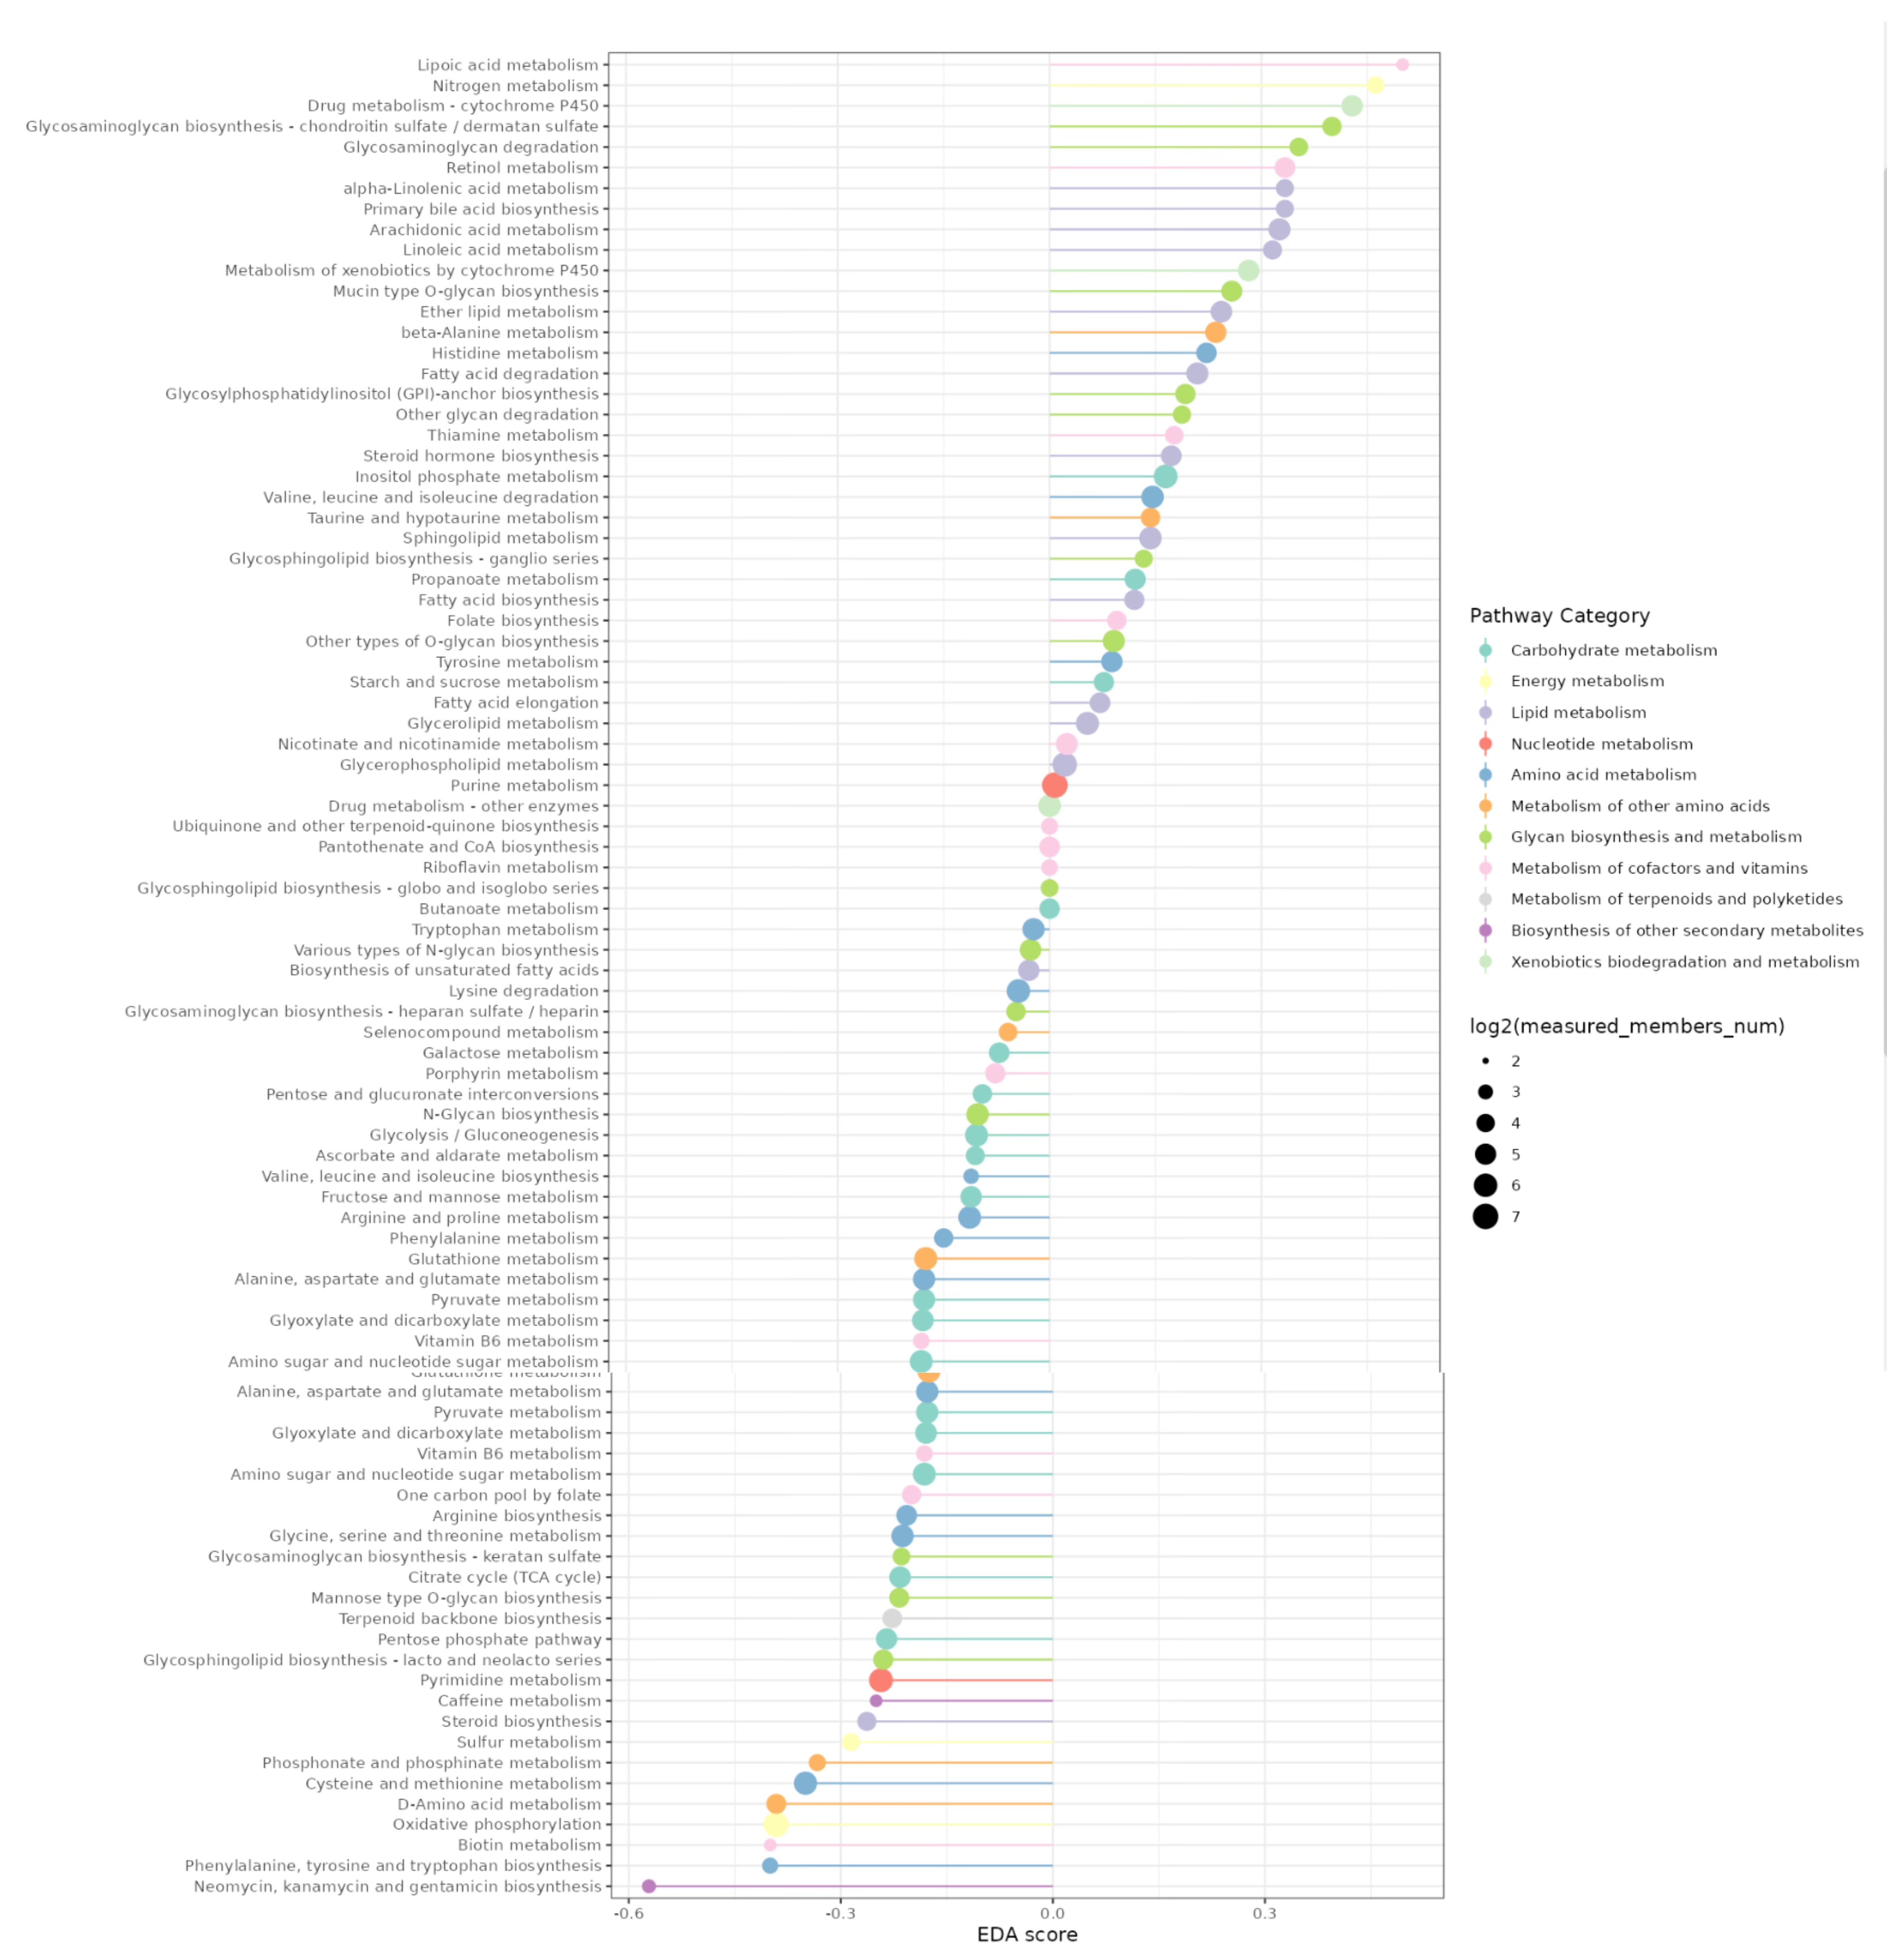
\includegraphics[width=0.7\linewidth]{figure/2.ePDA} \end{center}

Figure 1. ePDA score captures the tendency for a pathway to exhibit increased or decreased levels of genes and metabolites that are statistically significant differences between two group.

\section{eSEA}\label{esea}

Extended pathway set enrichment analysis

\subsection{Interface}\label{interface-3}

\textbf{Procedure}

Step 1: Enter \textbf{Metabolite Data}, \textbf{GeneExp Data} and \textbf{Group Data}, respectively.

Step 2: Select \textbf{Log(FoldChange), Padjust Cutoff and Pathway Pcutoff}, respectively.

\textbf{Fold change}: Identifies key metabolites with significant expression shifts between conditions, revealing potential metabolic alterations and pathway involvement in biological processes.

\textbf{Padjust Cutoff}: Helps filter significant results by controlling for false positives, ensuring that only statistically robust pathways are identified for further investigation.

\textbf{Pathway Pcutoff}: Sets a significance threshold, helping to identify pathways with meaningful changes while reducing the likelihood of false-positive findings.

Step 3: Select \textbf{Figure Format} and adjust \textbf{figure width, height and DPI}.

Step 4: Click the \textbf{User} panel to \textbf{view the input and output}, and finally click \textbf{Figure Download} and export the analysis results.

\begin{center}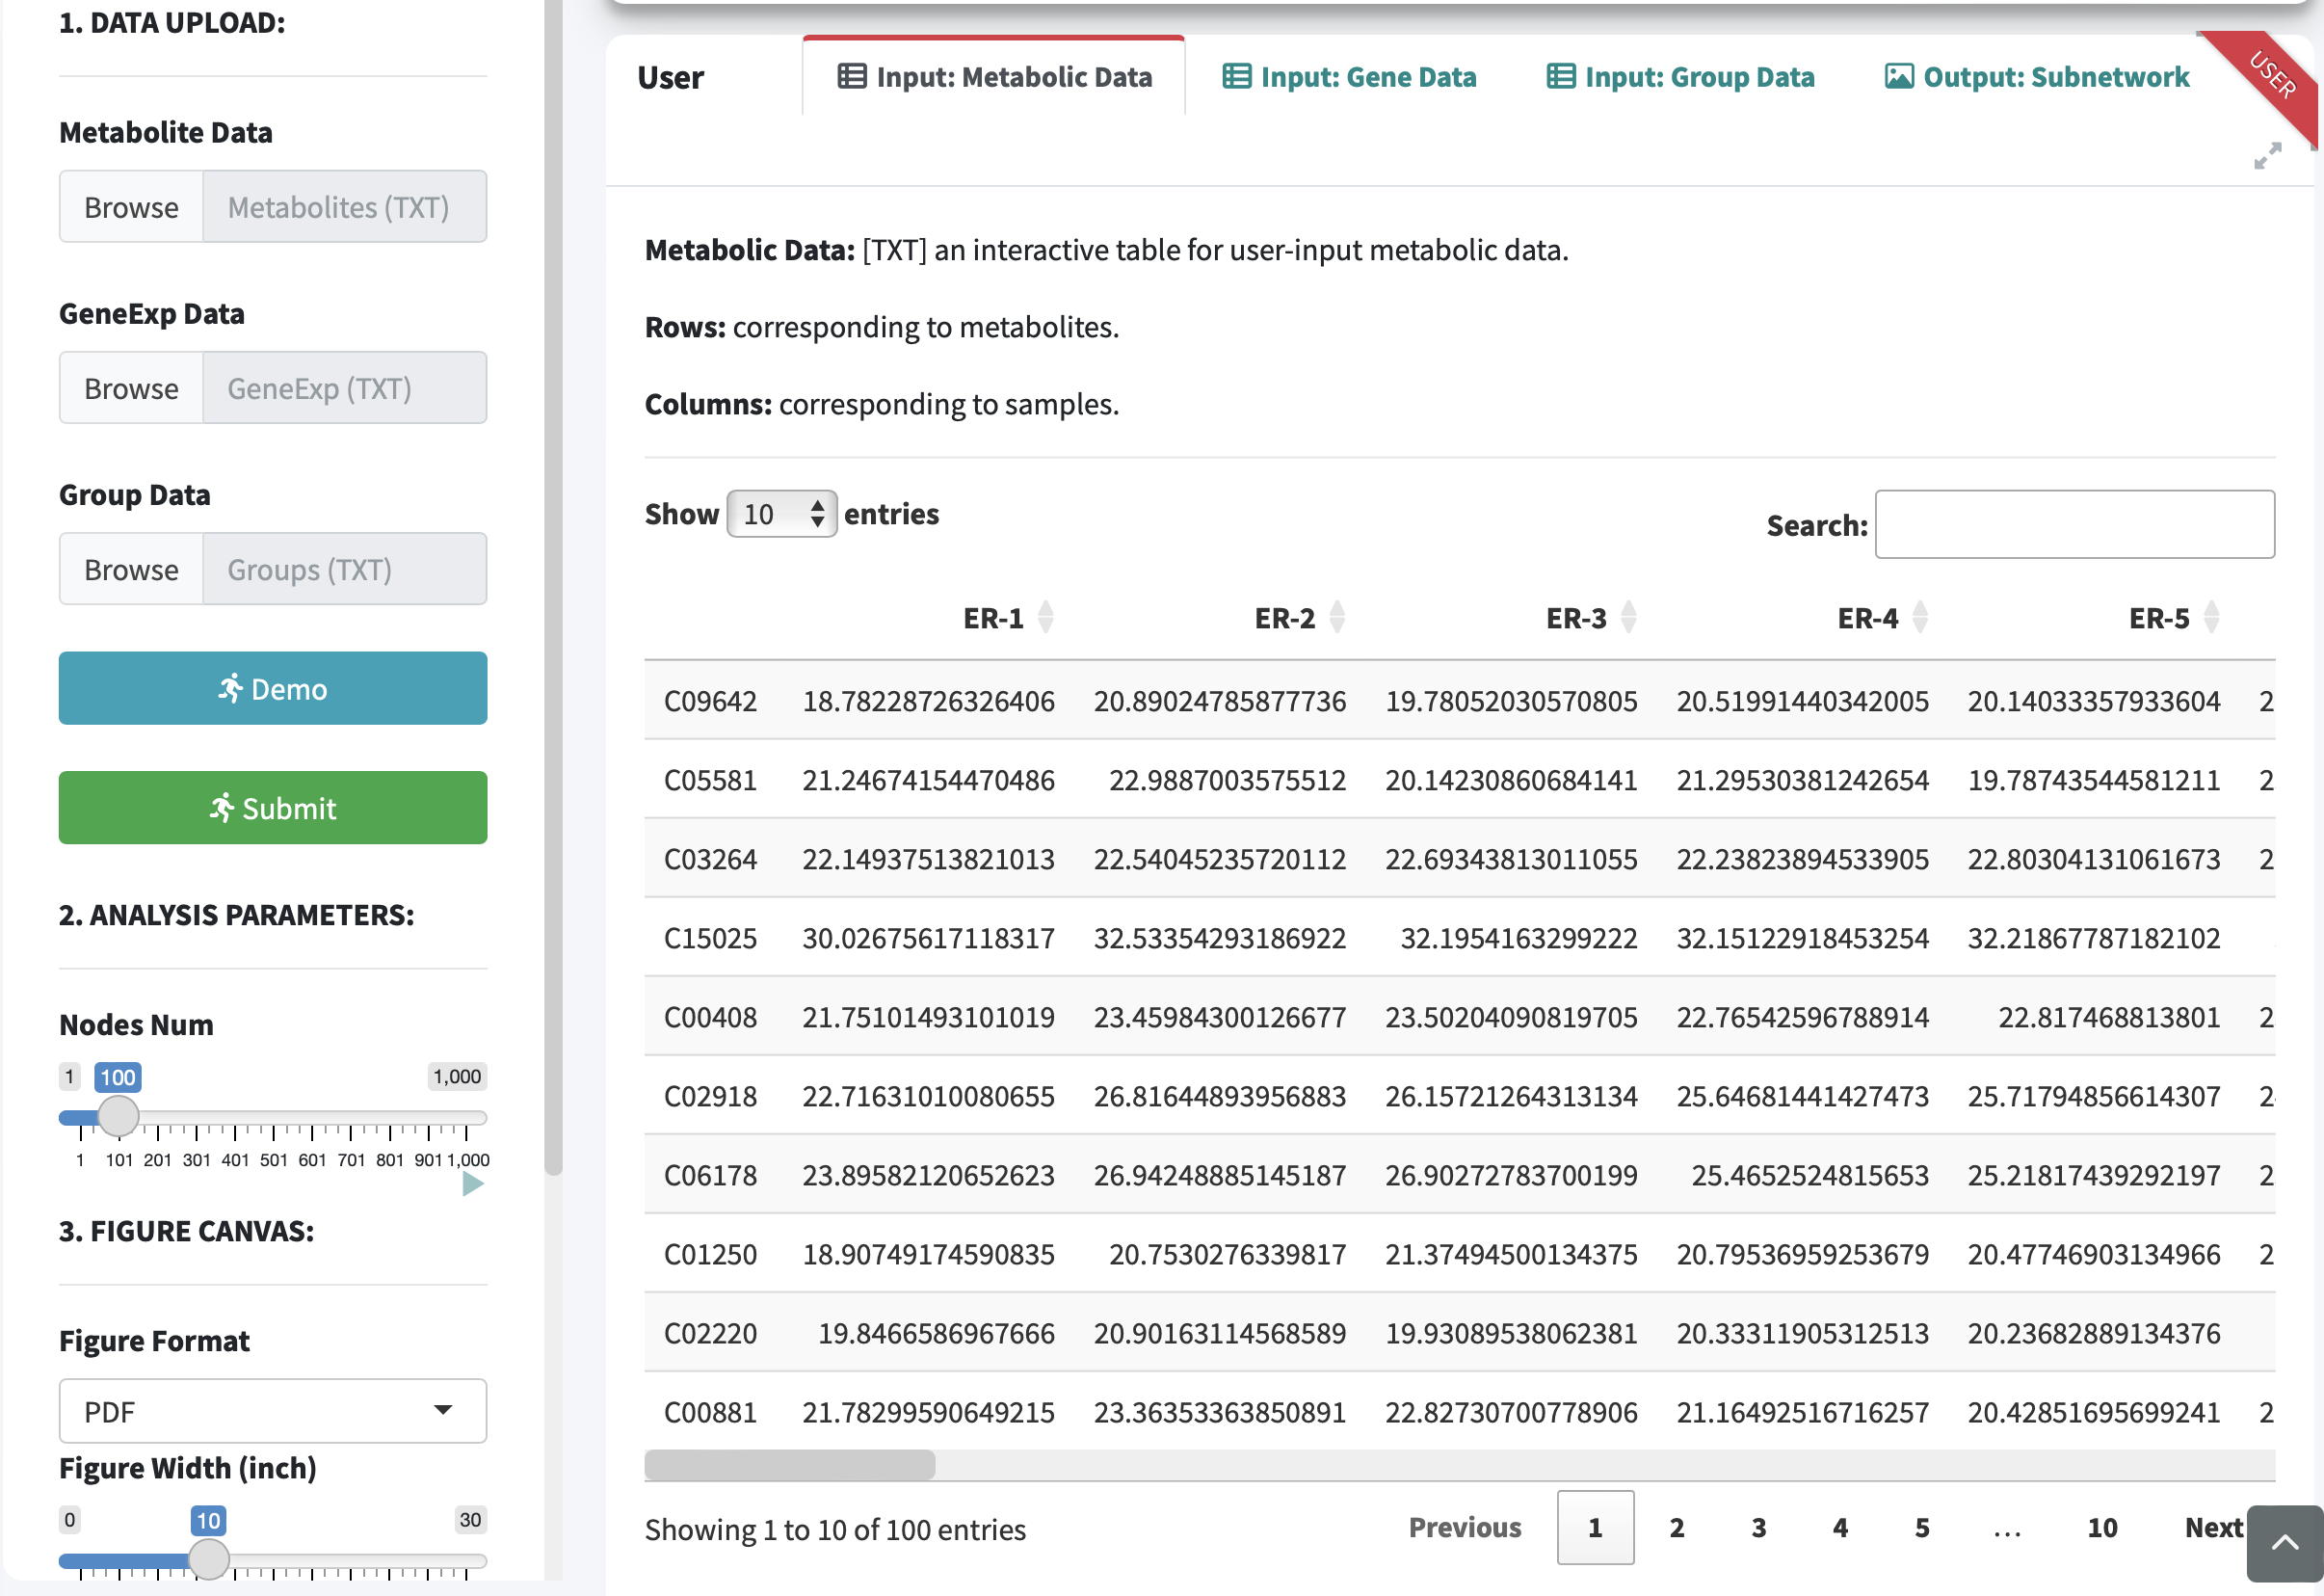
\includegraphics[width=33.5in]{figure/1.M-G} \end{center}

\textbf{Demo data}

\textbf{Expand the Demo Panel and click Metabolic Data to download demo data}, which comprises an integrated analysis of metabolomic and transcriptomic profiles in triple-negative breast cancer.

\textbf{Metabolite Data}: an interactive table for user-input metabolic data with rows corresponding to metabolites and columns corresponding to samples.

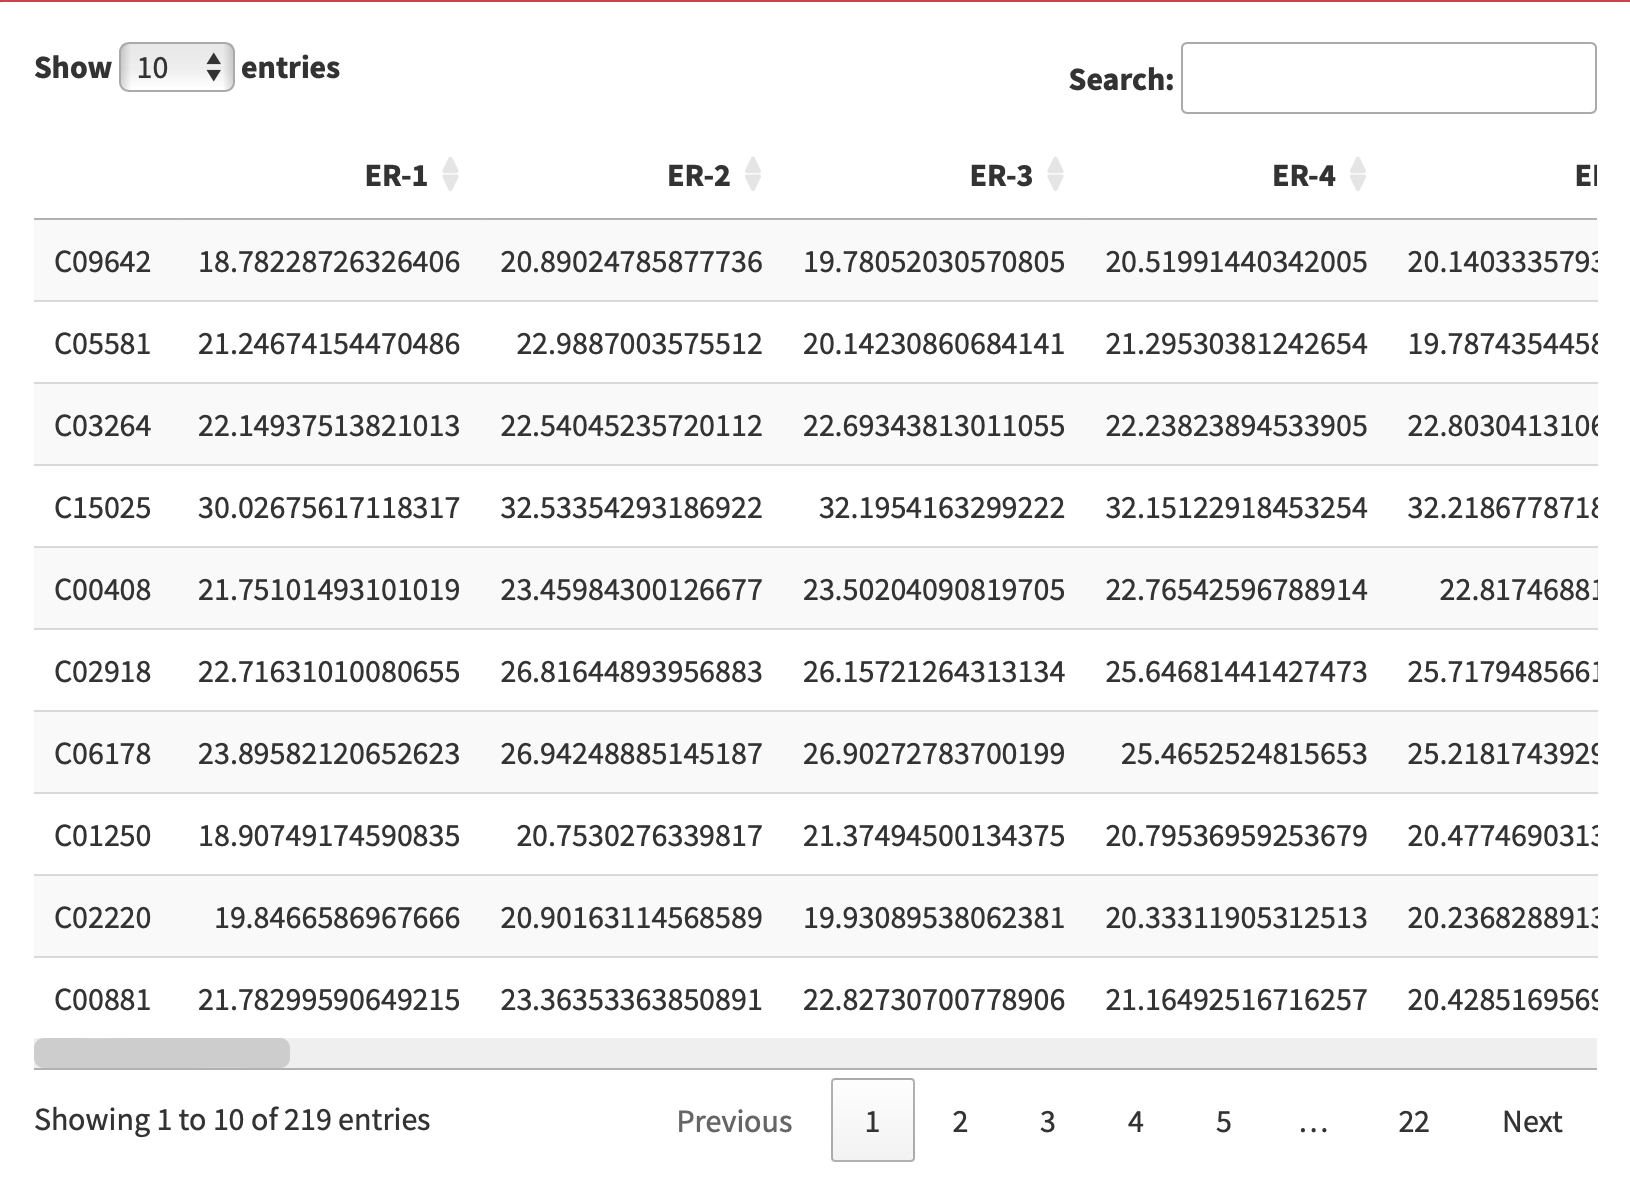
\includegraphics[width=22.64in]{figure/Metabolite}

\textbf{GeneExp Data}: an interactive table for user-input metabolic data with rows corresponding to genes and columns correspond to the samples.

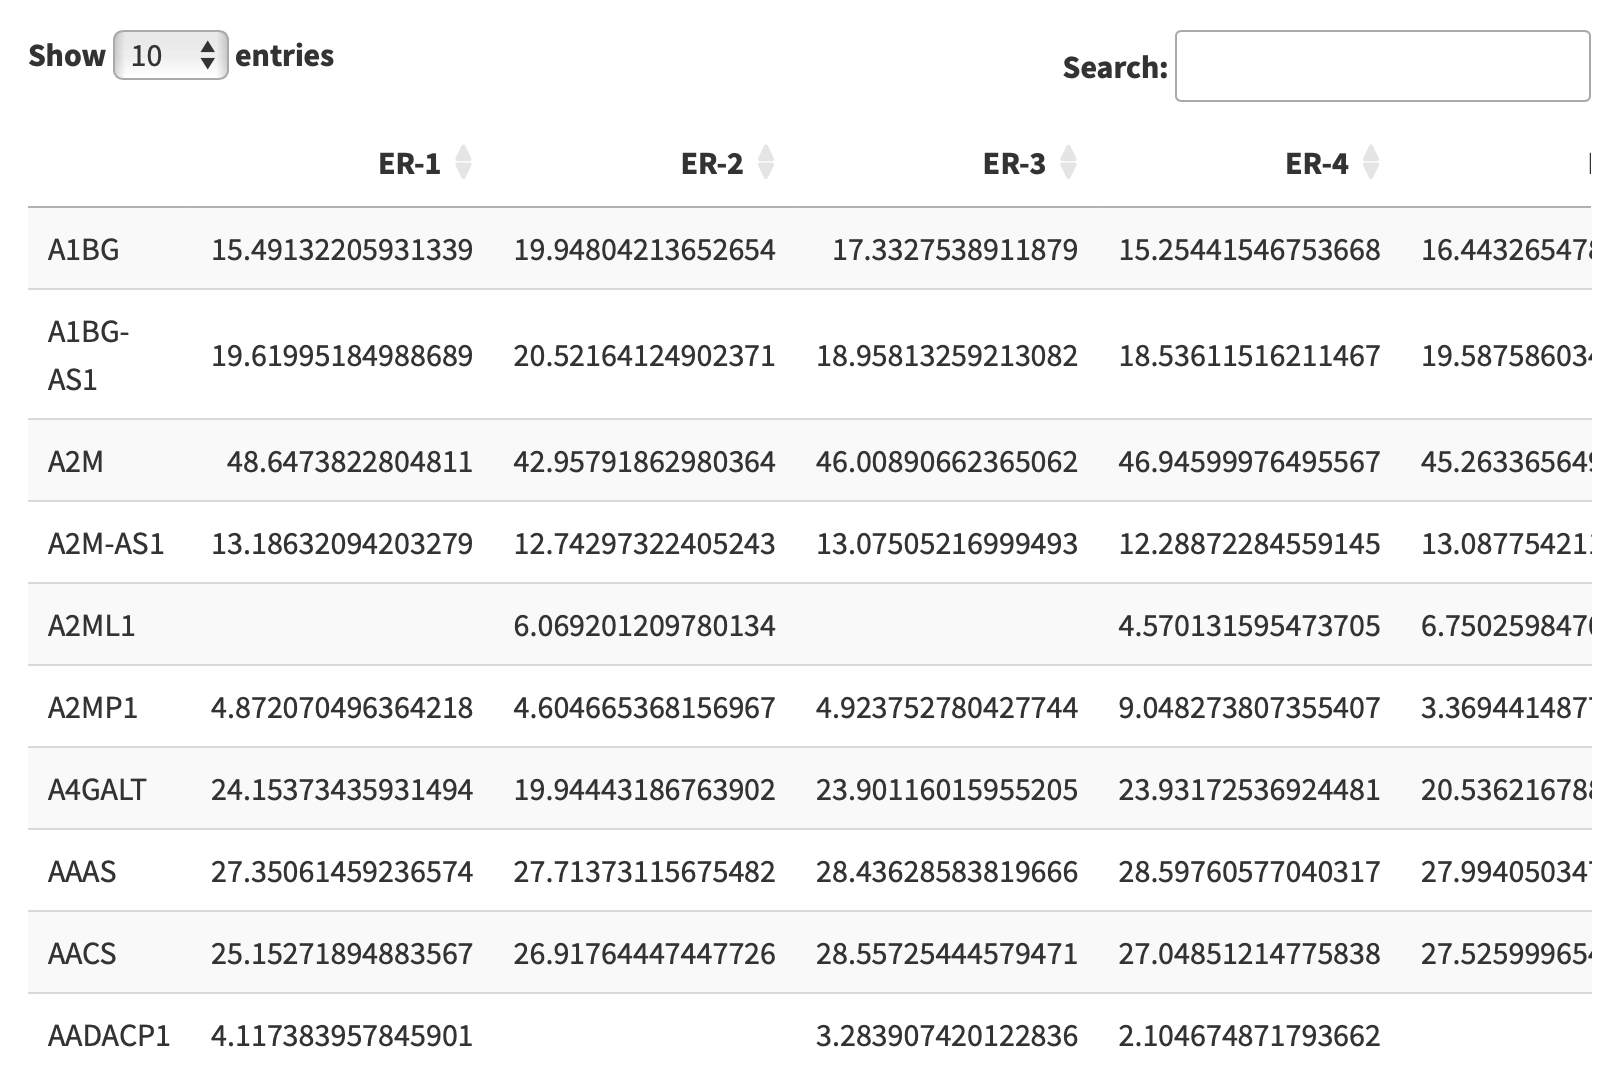
\includegraphics[width=22.42in]{figure/GeneExp}

\textbf{Group Data}: Group information.

\begin{flushleft}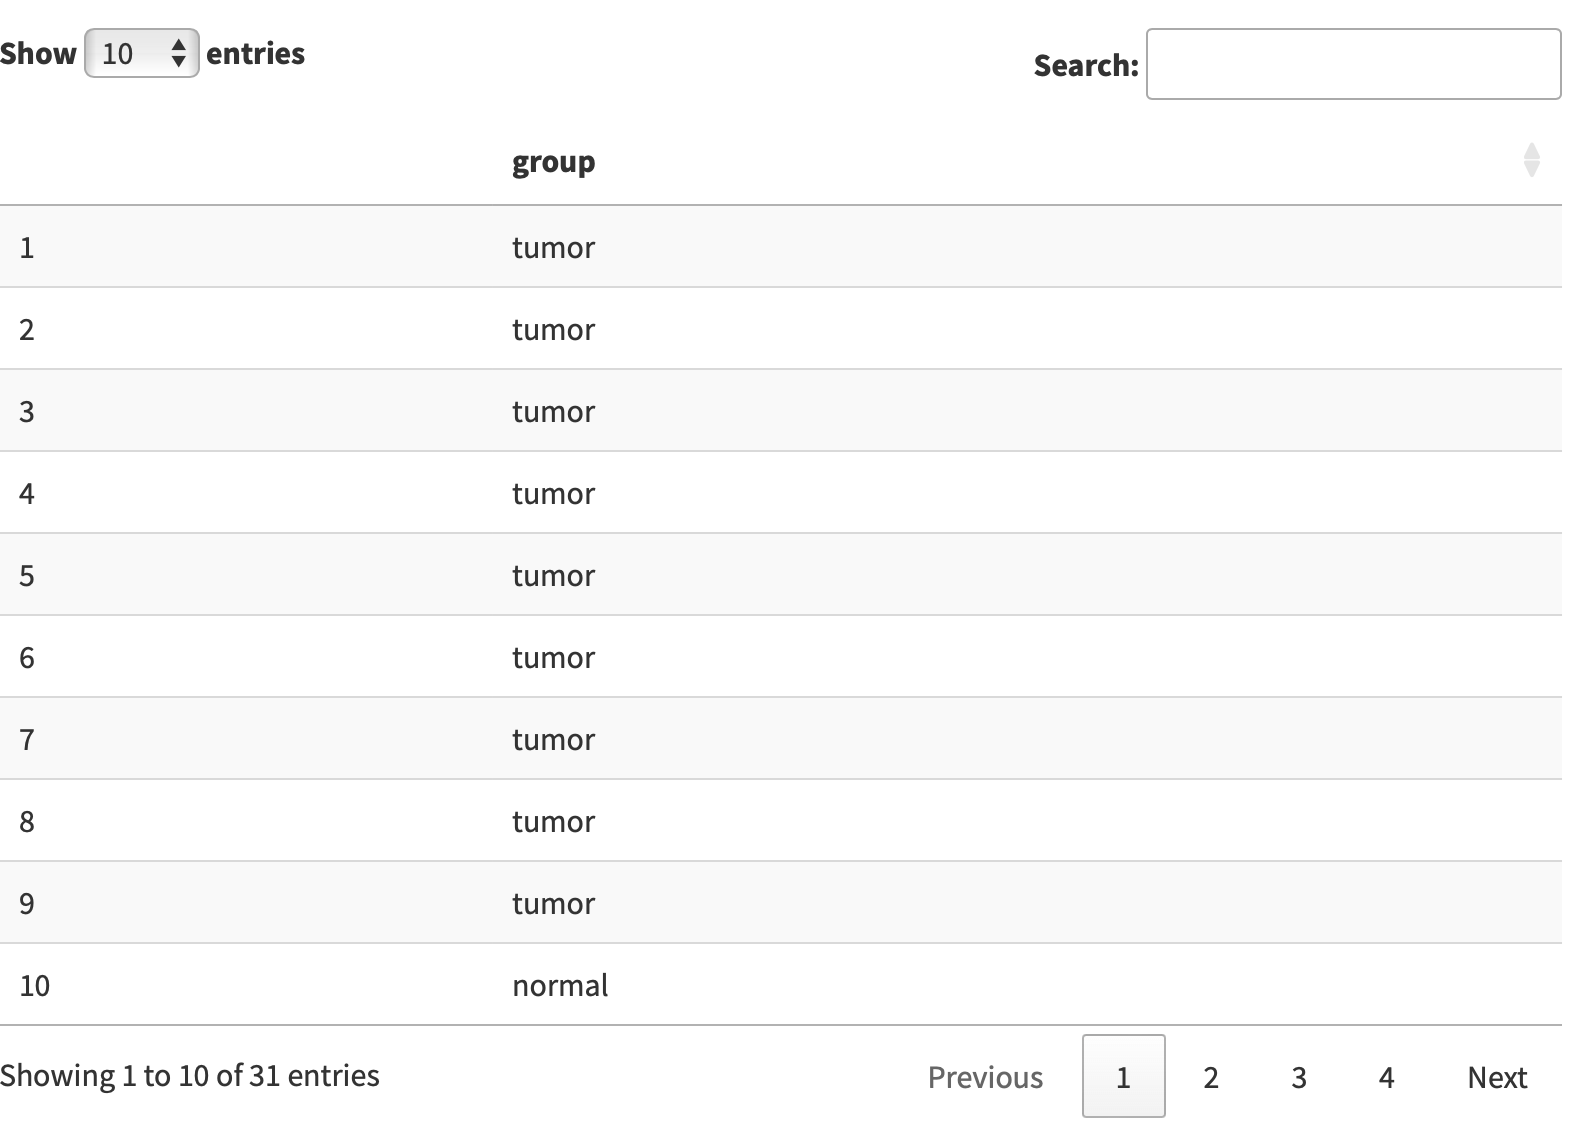
\includegraphics[width=21.83in]{figure/GroupInfo} \end{flushleft}

\subsection{Results}\label{results-3}

\begin{center}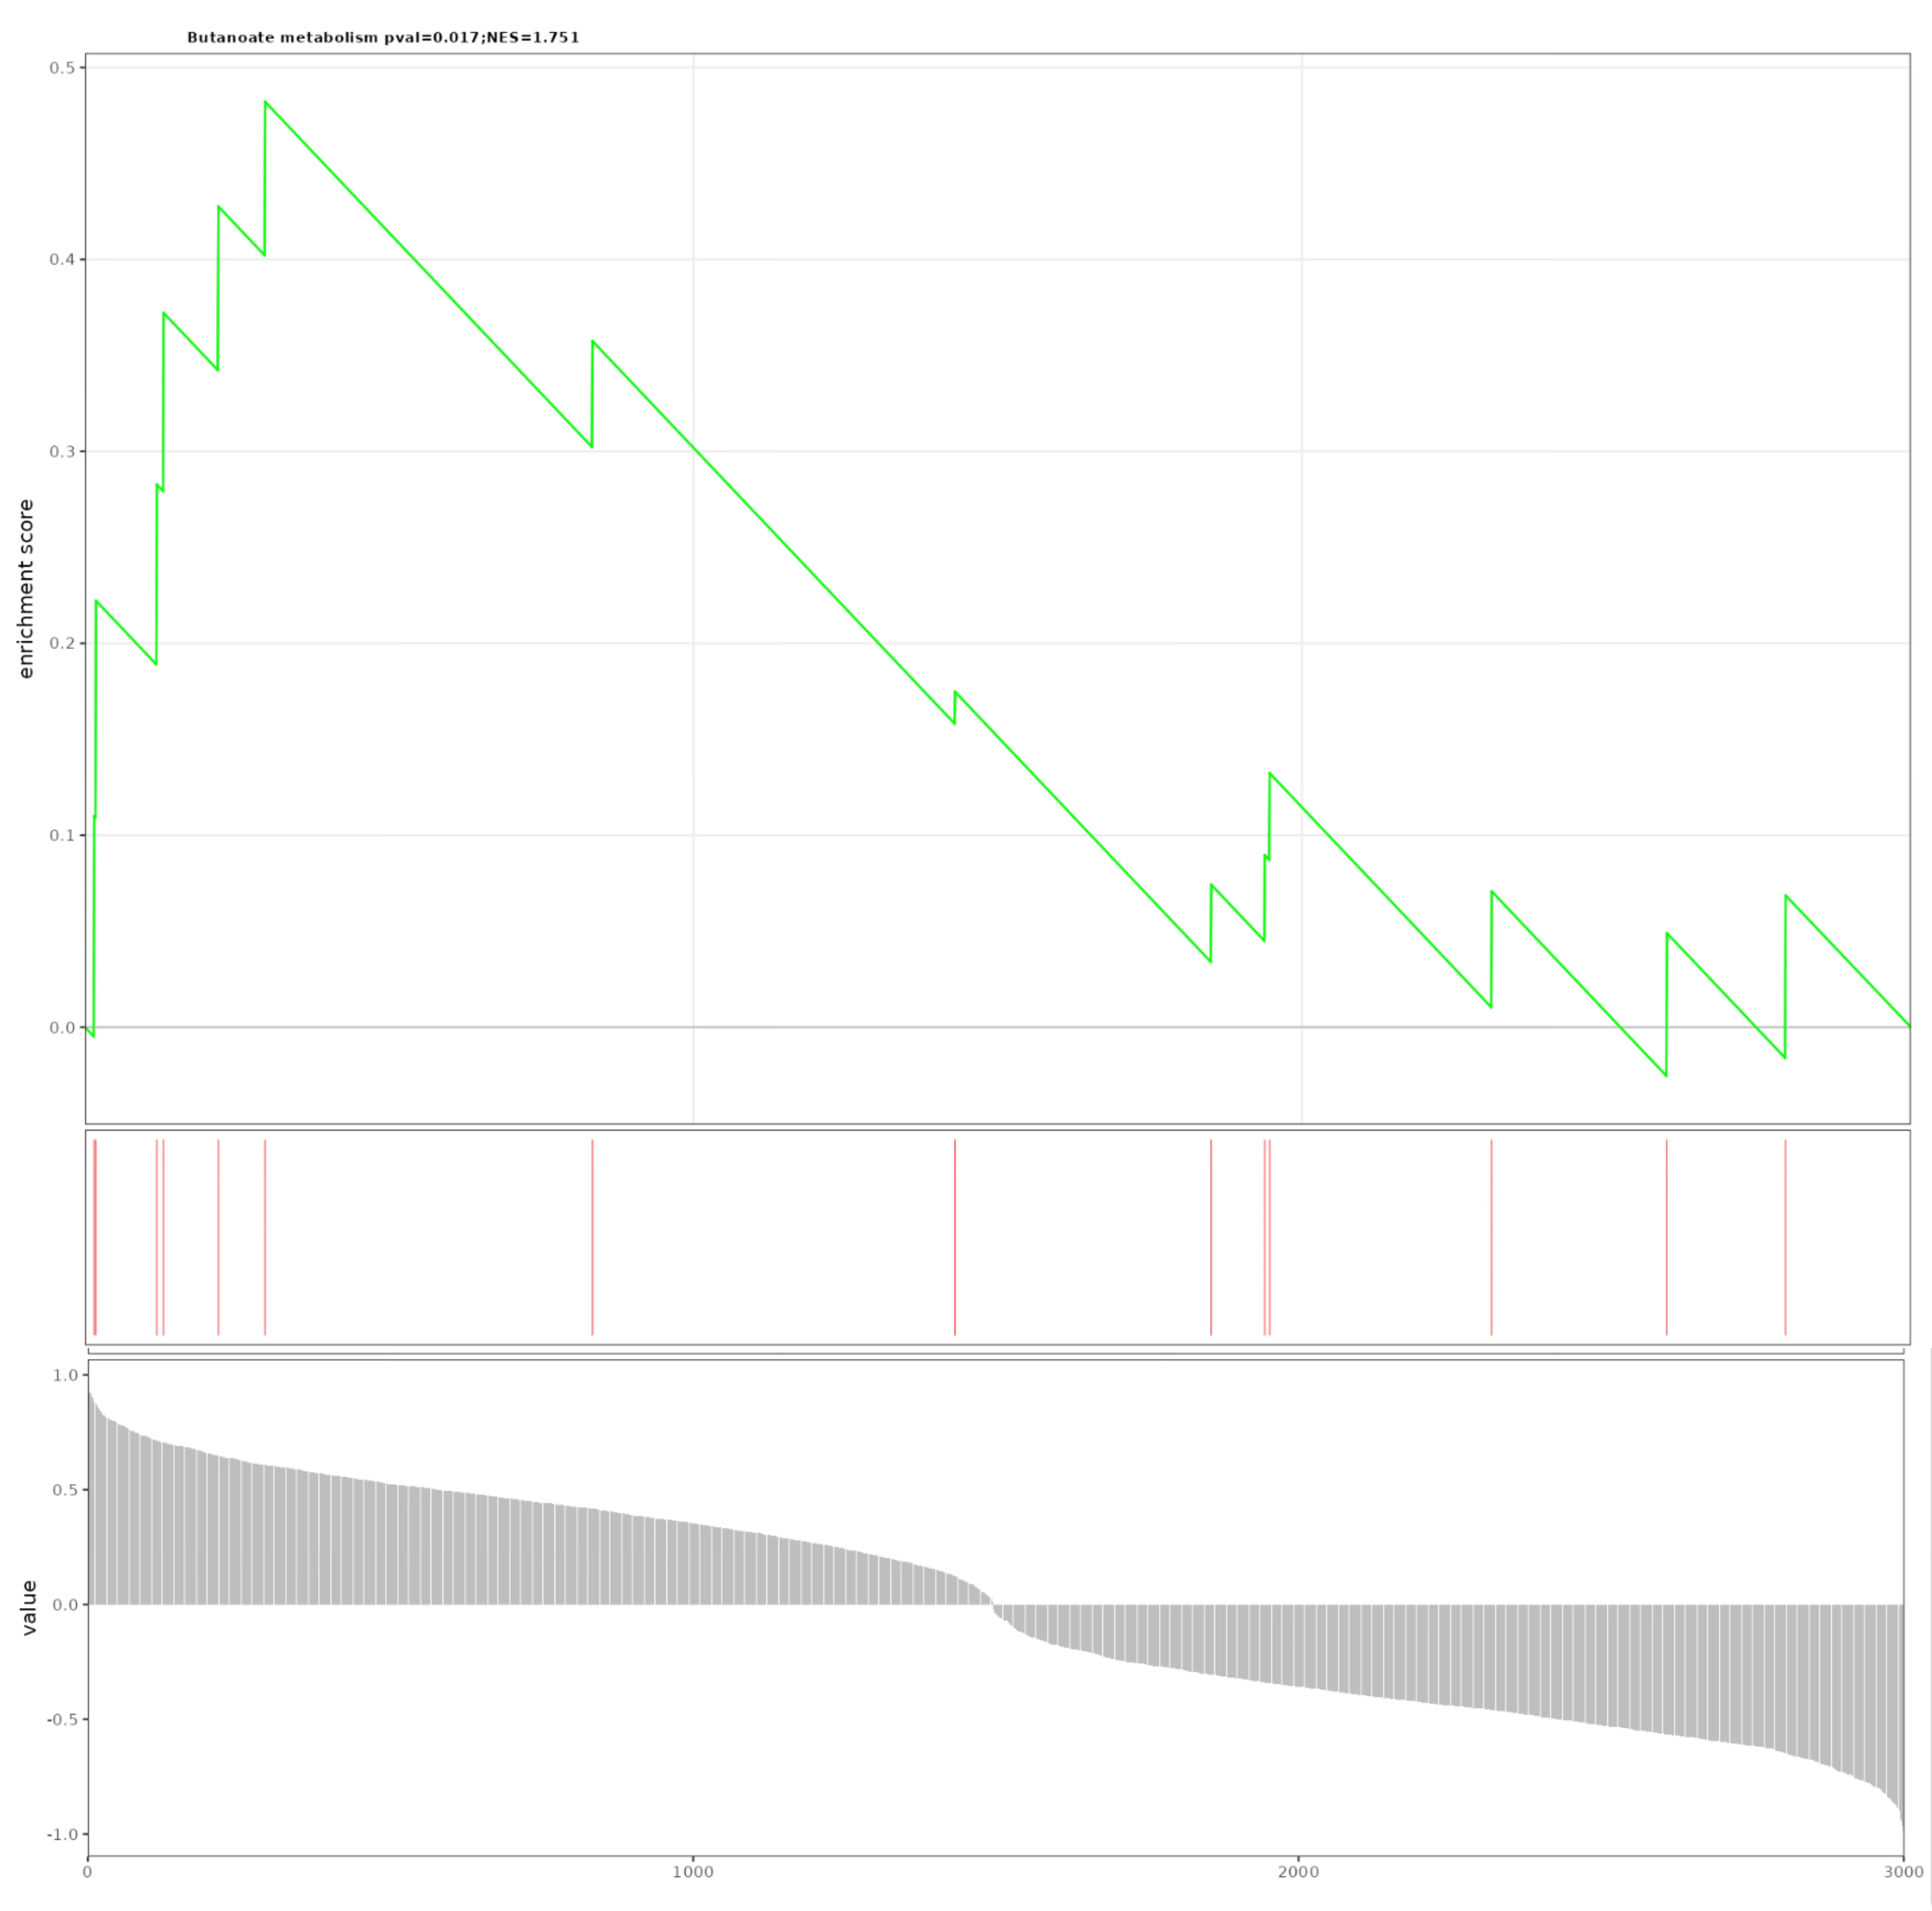
\includegraphics[width=0.6\linewidth]{figure/2.eSEA} \end{center}

Figure 1. Extended pathway set enrichment analysis.

\chapter{Deployment}\label{deployment}

\href{https://github.com/tuantuangui/MNet}{MNet Source Files}

\href{http://www.mnet4all.com/MNet/}{MNet Web server}

\section{Installing R 4.4.1 for Ubuntu 20}\label{installing-r-4.4.1-for-ubuntu-20}

\begin{center}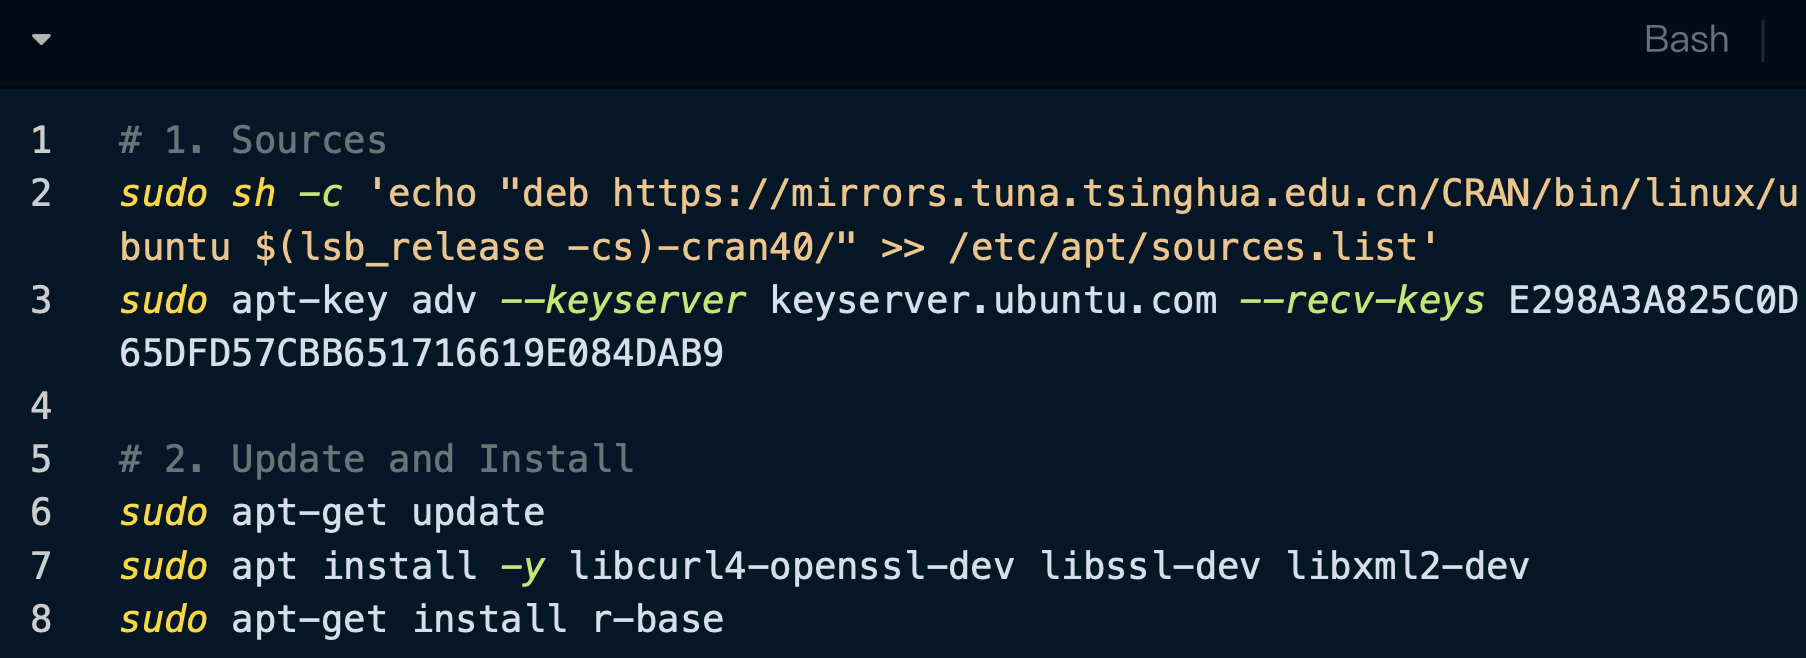
\includegraphics[width=25.08in]{figure/3.1} \end{center}

\section{Installing R Packages}\label{installing-r-packages}

\begin{center}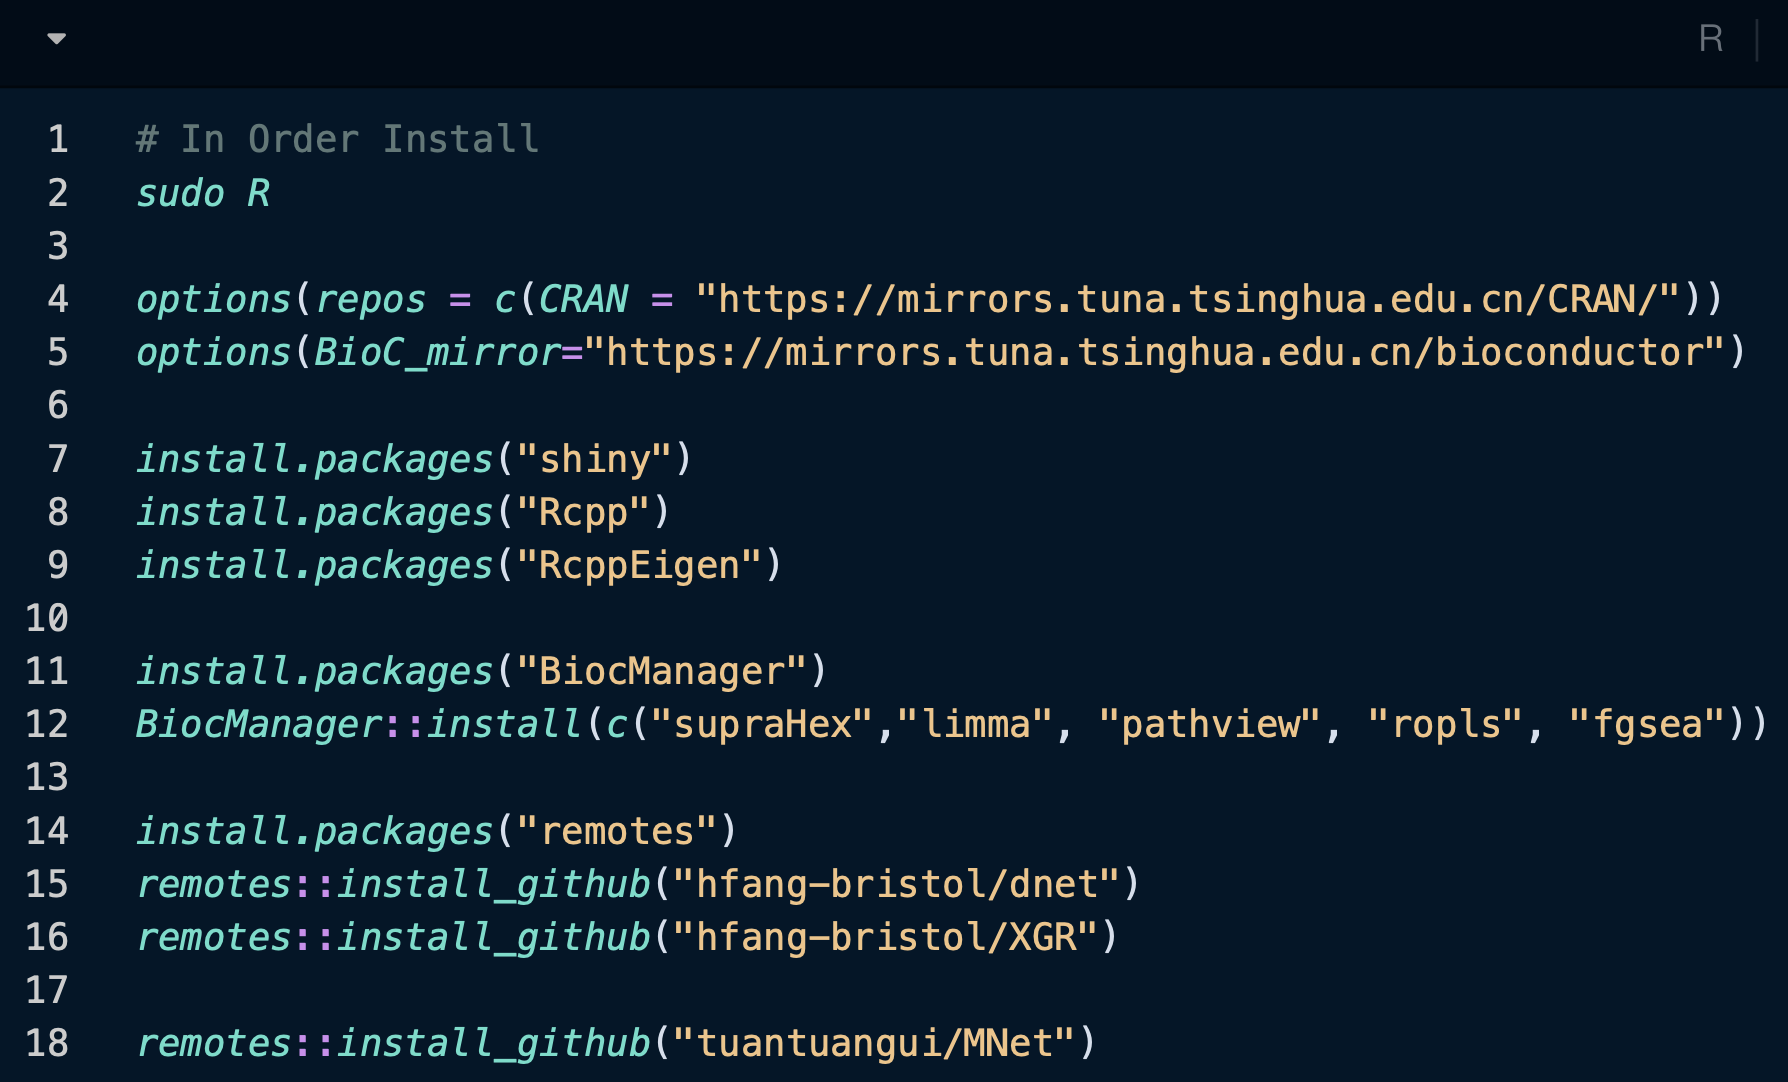
\includegraphics[width=24.83in]{figure/3.2} \end{center}

\section{Installing shiny-sever}\label{installing-shiny-sever}

\begin{center}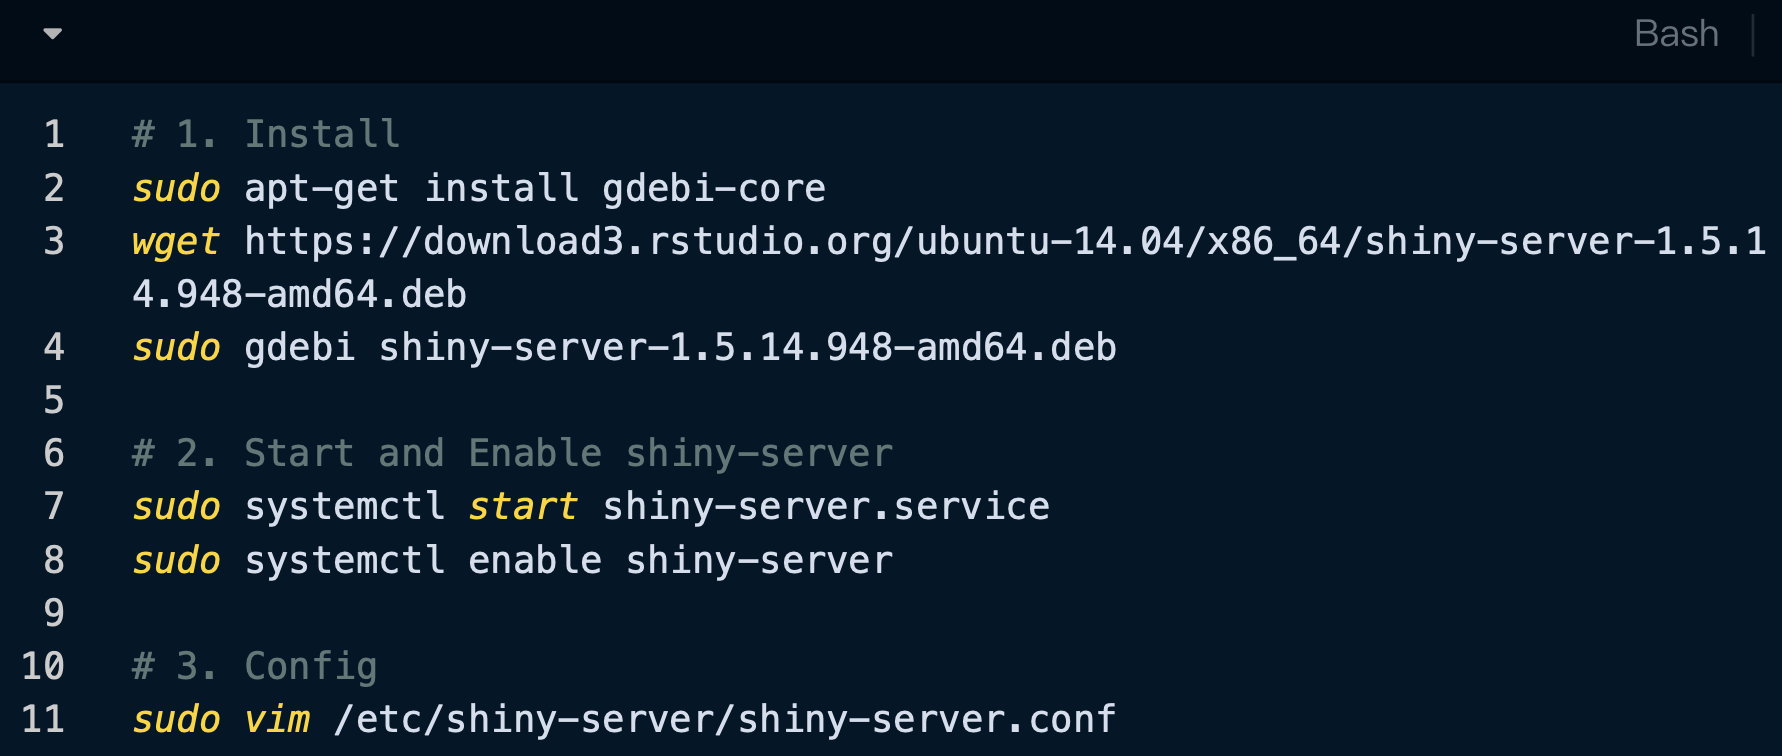
\includegraphics[width=24.75in]{figure/3.3.1} \end{center}

\begin{center}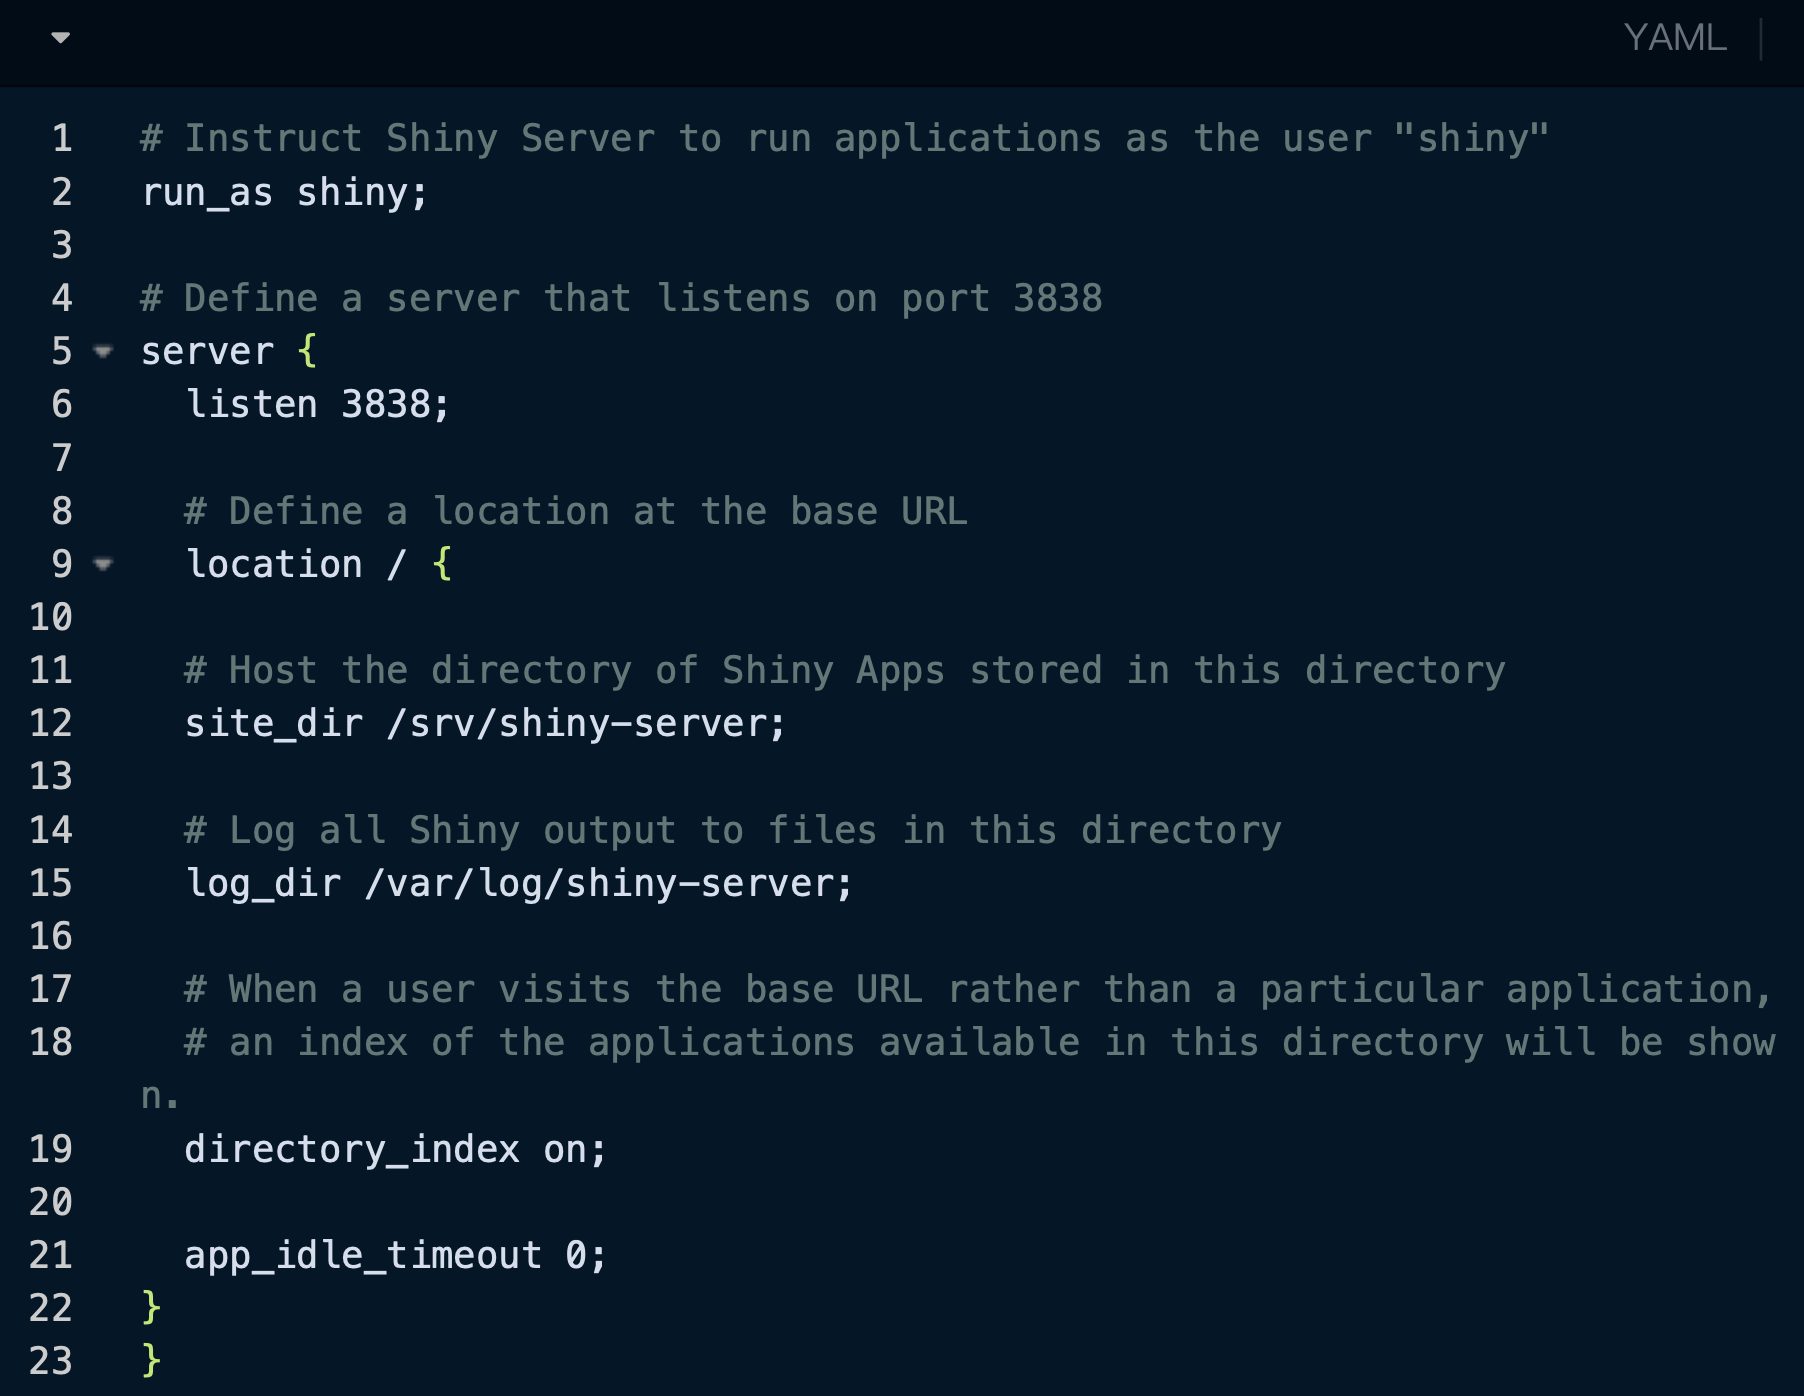
\includegraphics[width=25.06in]{figure/3.3.2} \end{center}

\section{Shiny App Server and Logs}\label{shiny-app-server-and-logs}

\begin{center}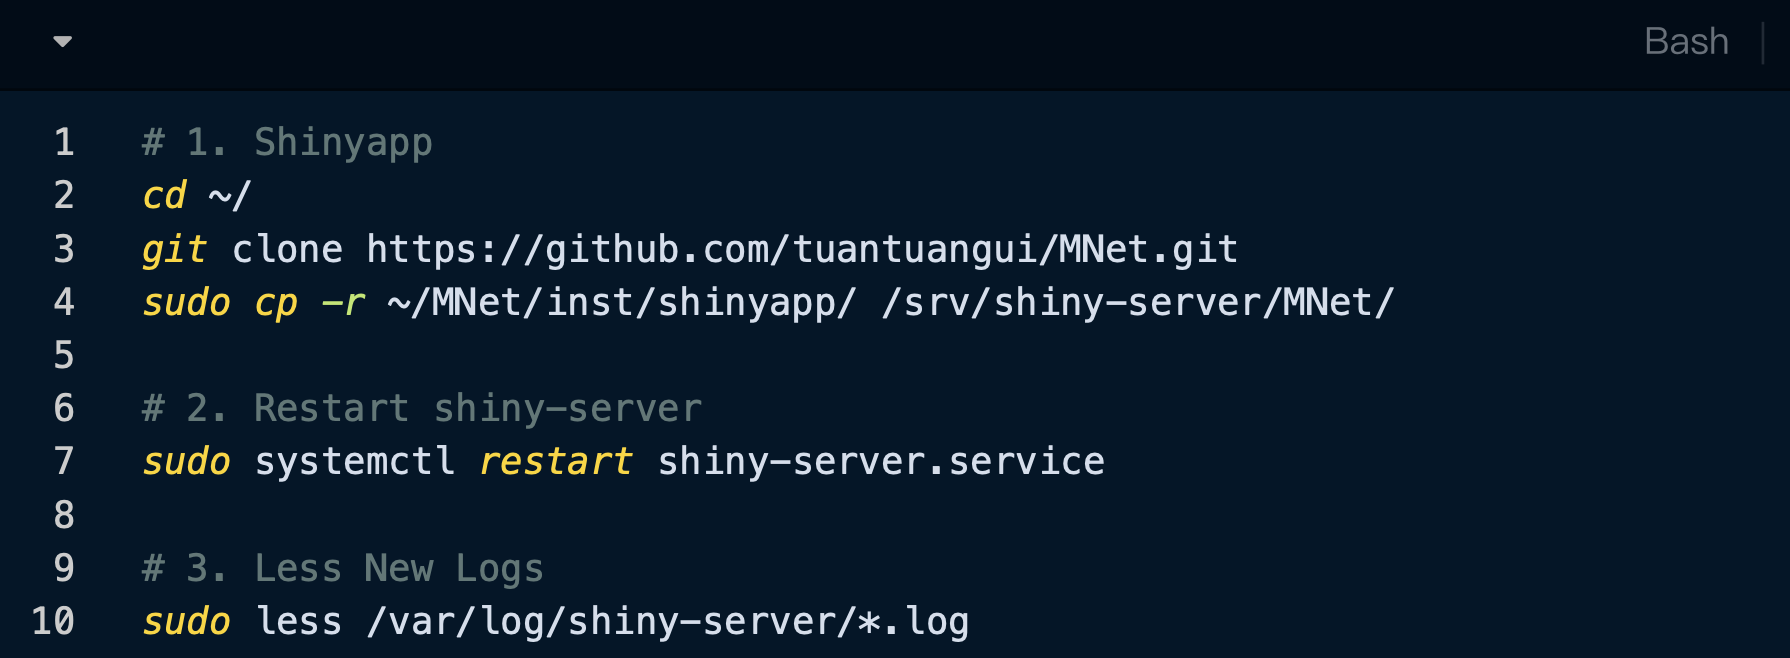
\includegraphics[width=24.86in]{figure/3.4.1} \end{center}

\section{Firewall: firewalld or ufw}\label{firewall-firewalld-or-ufw}

\begin{center}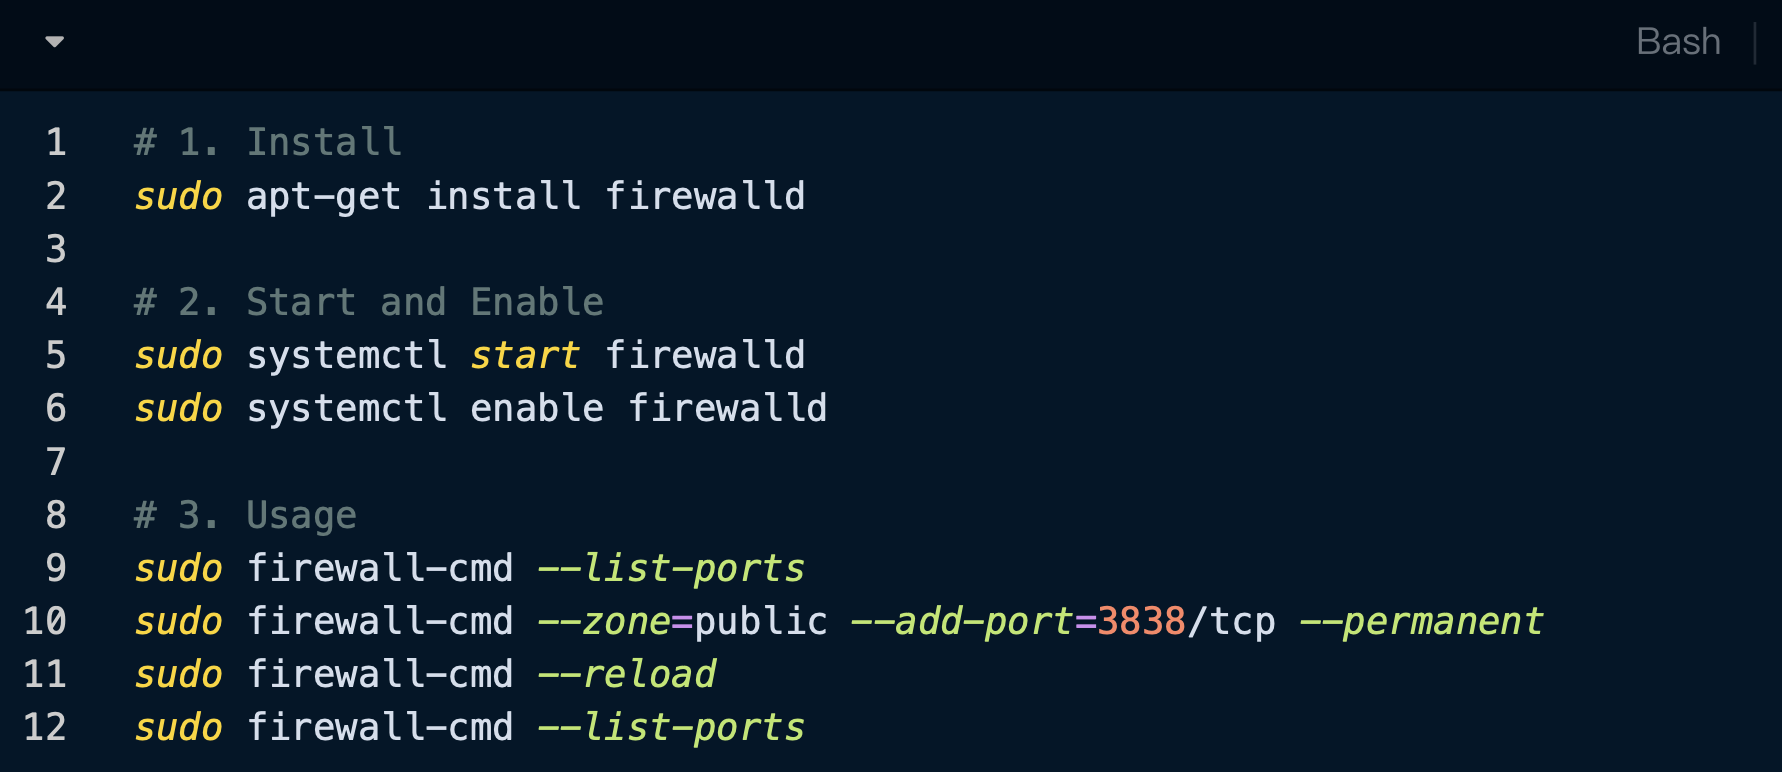
\includegraphics[width=24.75in]{figure/3.5.1} \end{center}

\begin{center}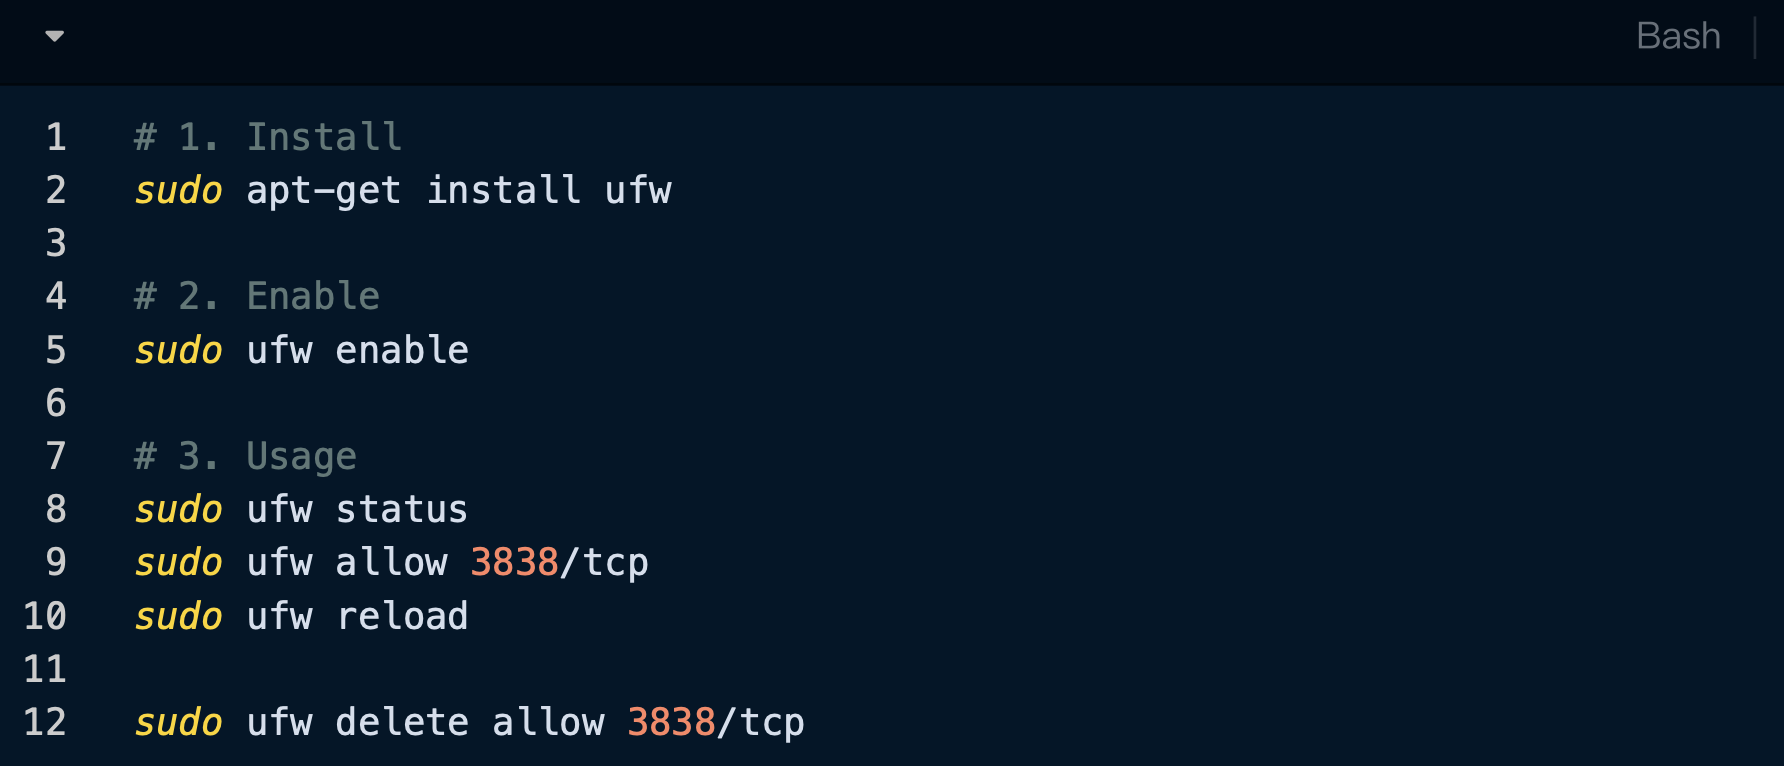
\includegraphics[width=24.78in]{figure/3.5.2} \end{center}

\section{Apache2 Config}\label{apache2-config}

\begin{center}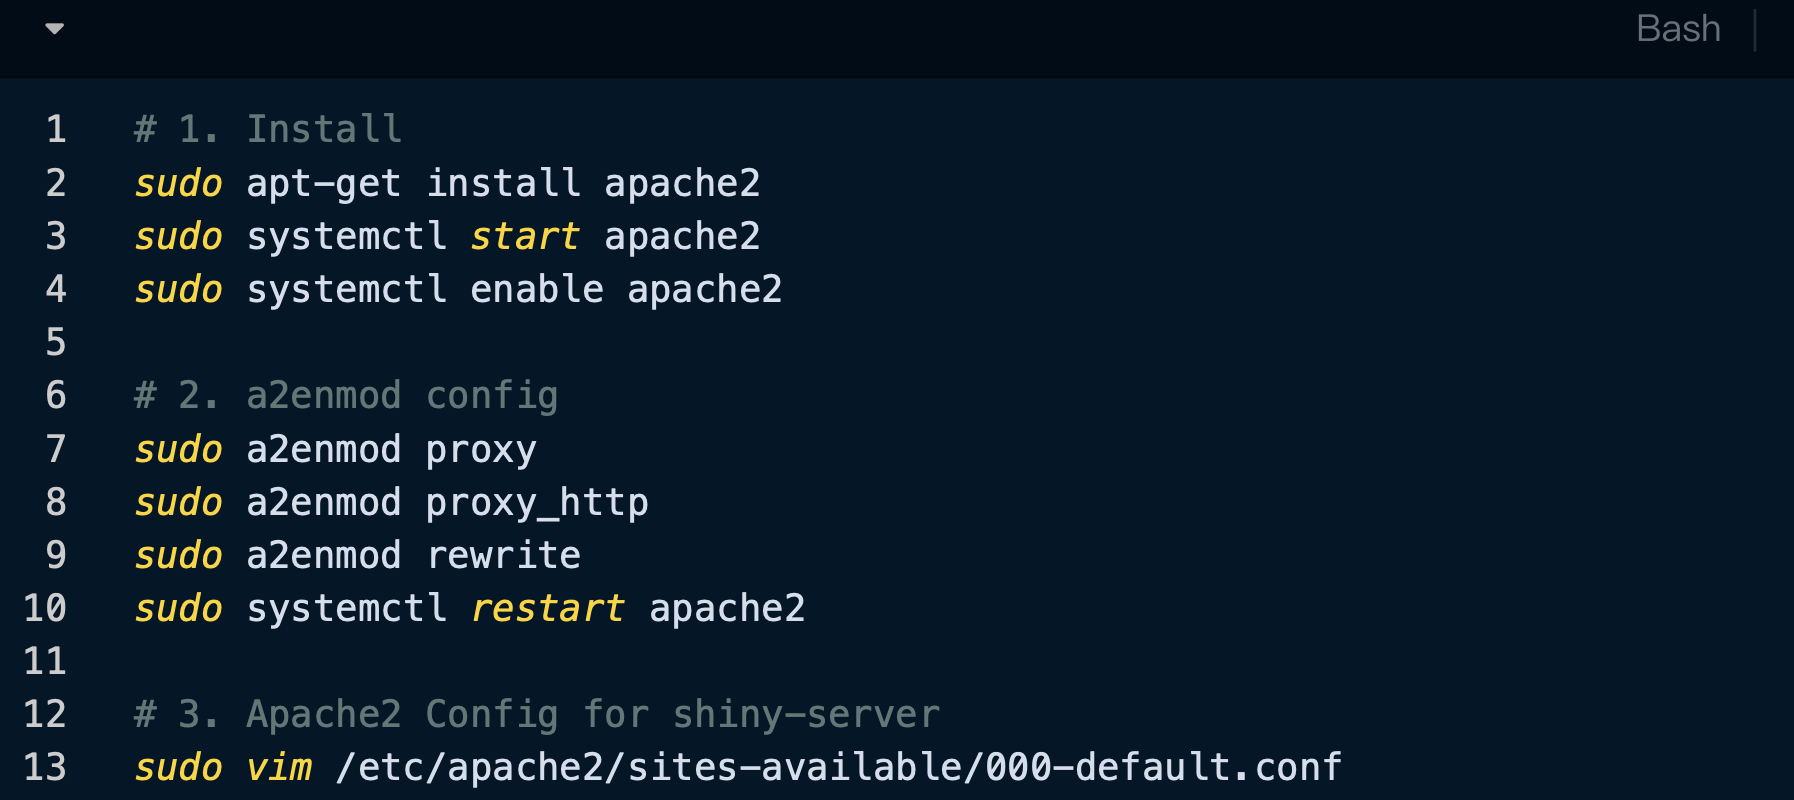
\includegraphics[width=24.92in]{figure/3.6.1} \end{center}

\begin{center}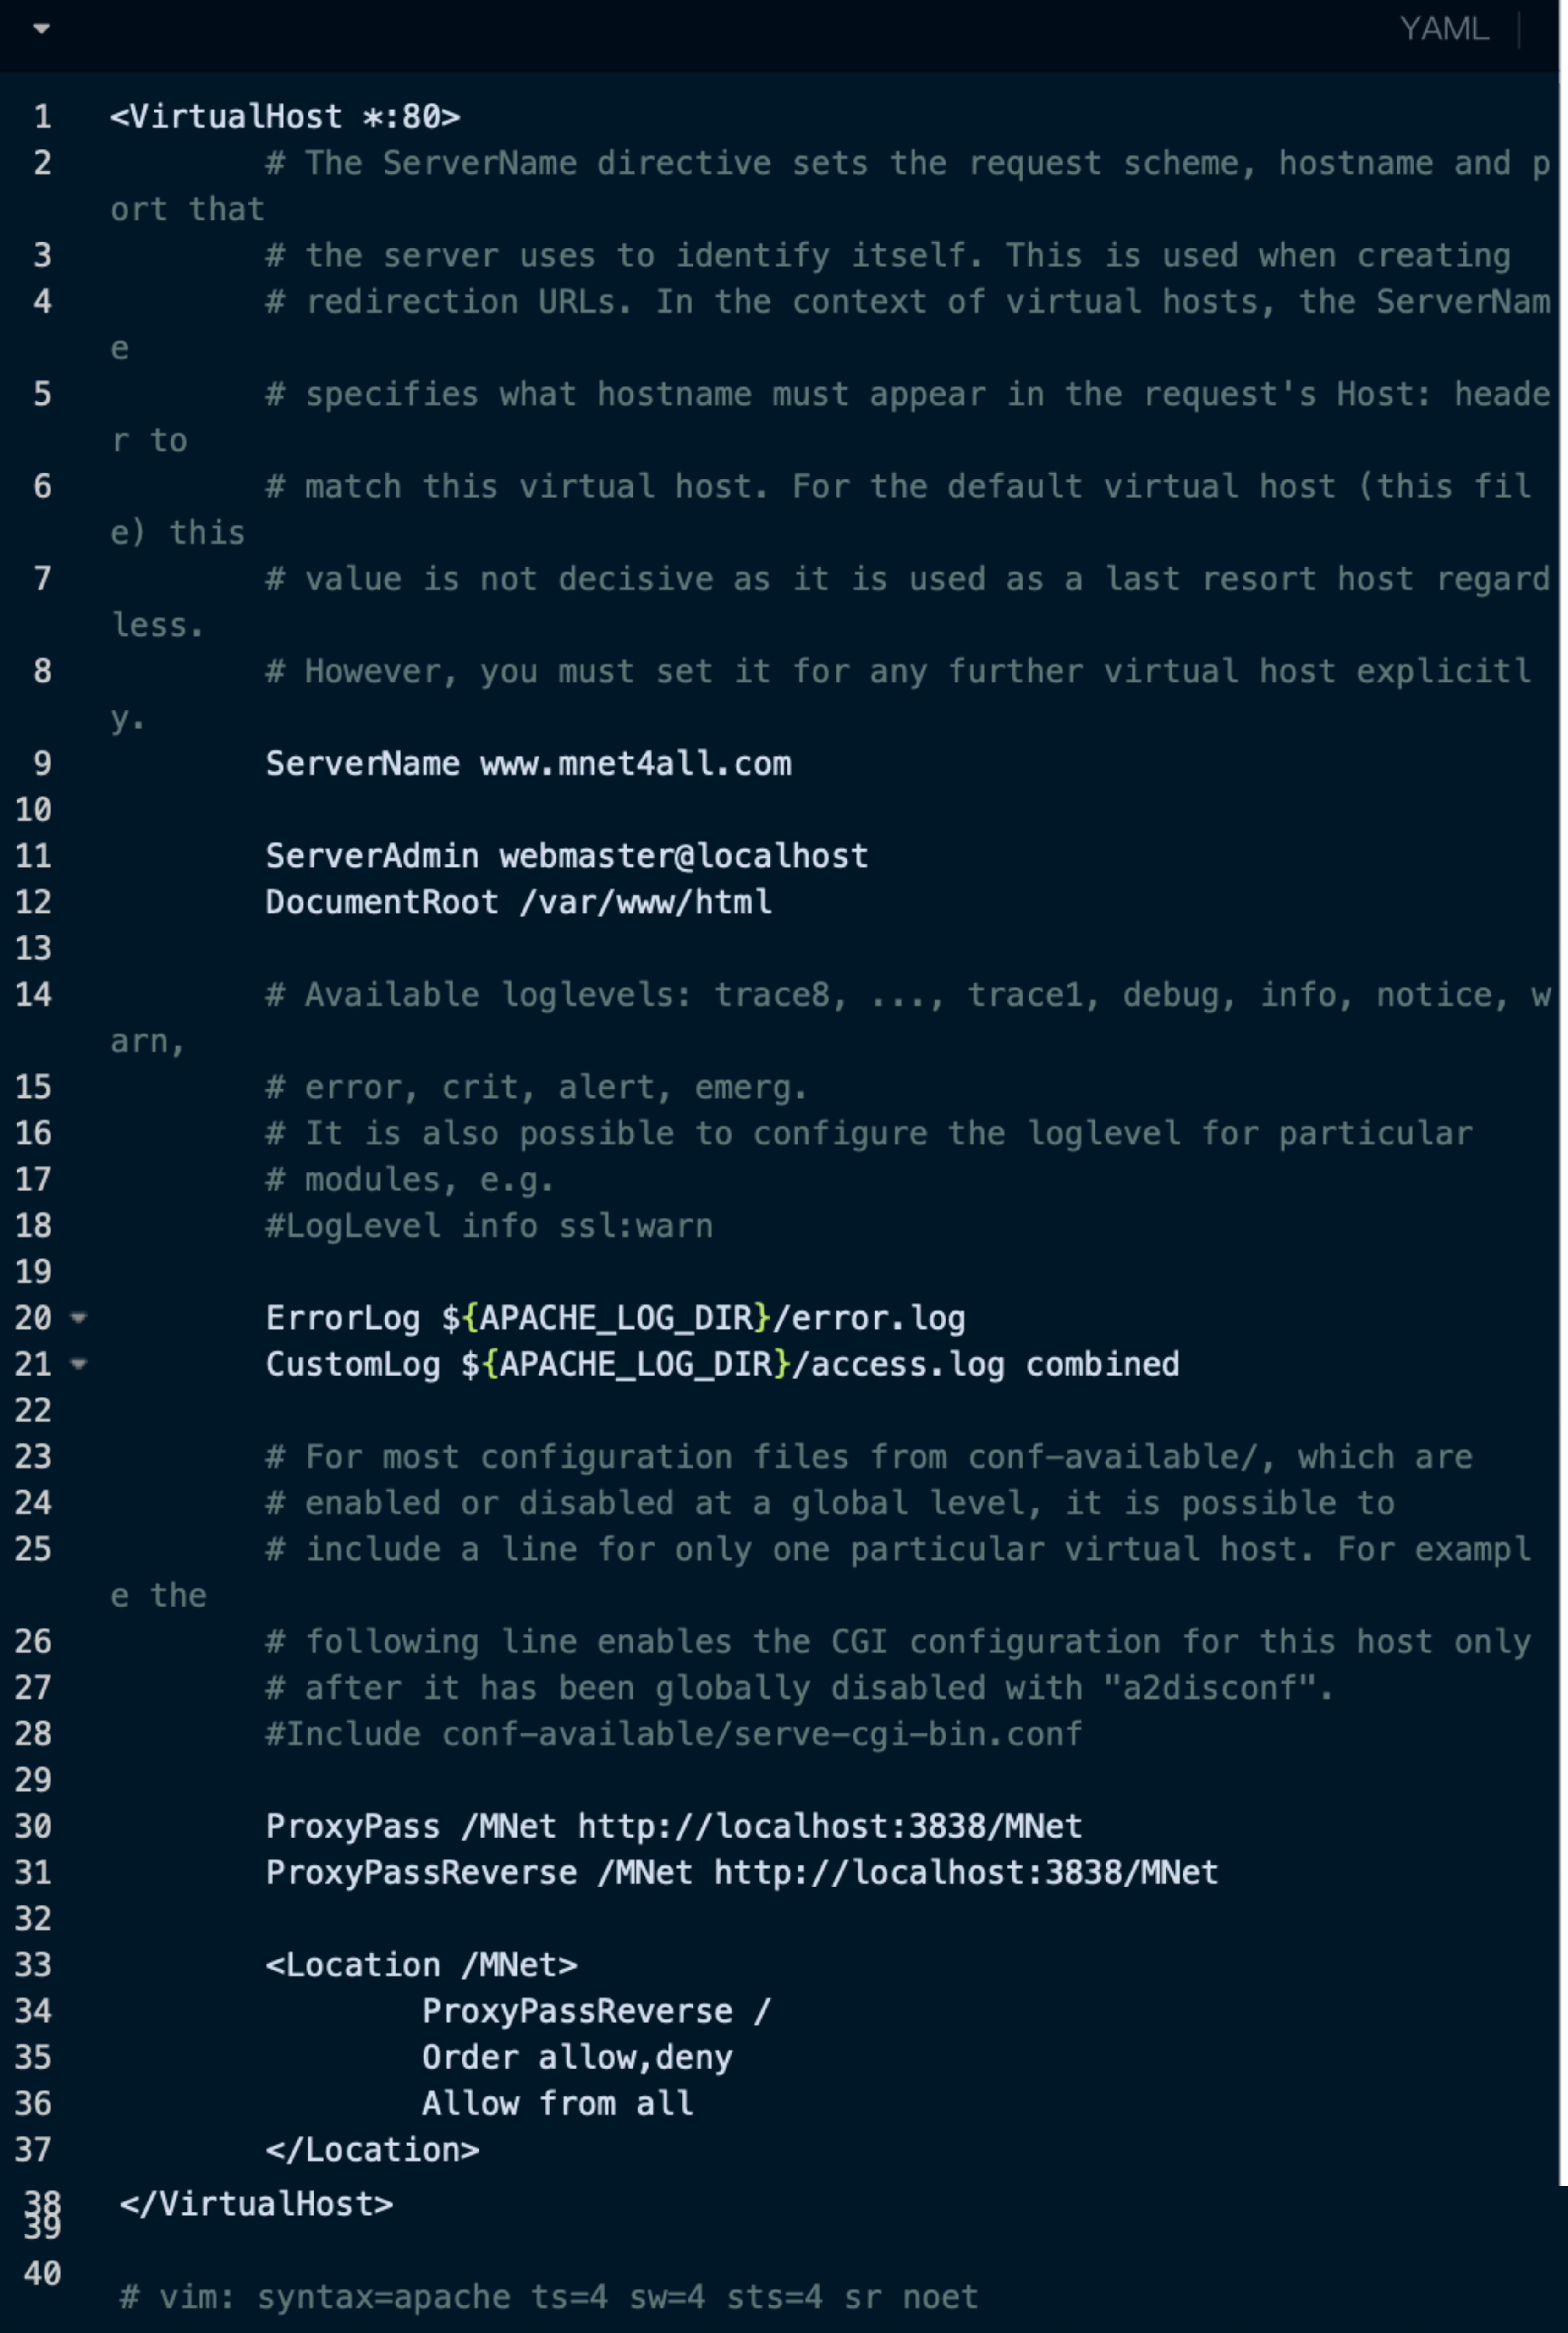
\includegraphics[width=47.51in]{figure/3.6.2} \end{center}

\begin{center}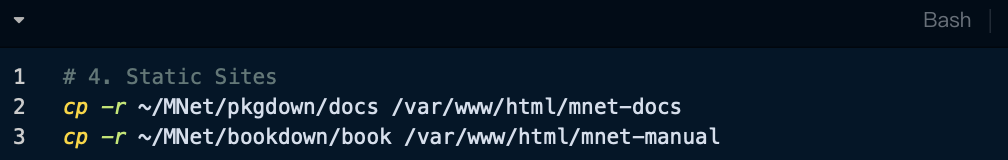
\includegraphics[width=1.5\linewidth]{figure/3.6.3} \end{center}

\chapter{dbMNet}\label{dbmnet}

dbKEGG for extended pathway analysis and dbNet for metabolism-related subnetwork analysis.

\section{KEGG pathway's metabolite and gene}\label{kegg-pathways-metabolite-and-gene}

This is the metabolites and the genes in every metabolism KEGG pathway.

\begin{Shaded}
\begin{Highlighting}[]
\FunctionTok{library}\NormalTok{(KEGGREST)}
\FunctionTok{library}\NormalTok{(dplyr)}

\DocumentationTok{\#\# All human metabolic pathways}
\NormalTok{pathway\_meta }\OtherTok{\textless{}{-}}\NormalTok{ data.table}\SpecialCharTok{::}\FunctionTok{fread}\NormalTok{(}\StringTok{"input/pathway\_hsa.txt"}\NormalTok{,}\AttributeTok{sep=}\StringTok{"}\SpecialCharTok{\textbackslash{}t}\StringTok{"}\NormalTok{,}\AttributeTok{header=}\NormalTok{F) }\SpecialCharTok{\%\textgreater{}\%}
  \FunctionTok{as.data.frame}\NormalTok{()}

\DocumentationTok{\#\# Extract corresponding genes and metabolites for each pathway}
\NormalTok{result\_gene }\OtherTok{\textless{}{-}} \FunctionTok{data.frame}\NormalTok{()}
\NormalTok{result\_compound }\OtherTok{\textless{}{-}} \FunctionTok{data.frame}\NormalTok{()}
\ControlFlowTok{for}\NormalTok{ (i }\ControlFlowTok{in} \DecValTok{1}\SpecialCharTok{:}\FunctionTok{length}\NormalTok{(pathway\_meta}\SpecialCharTok{$}\NormalTok{V2))\{}

  \FunctionTok{print}\NormalTok{(pathway\_meta}\SpecialCharTok{$}\NormalTok{V2[i])}

\NormalTok{  path }\OtherTok{\textless{}{-}} \FunctionTok{keggGet}\NormalTok{(pathway\_meta}\SpecialCharTok{$}\NormalTok{V2[i])}

  \DocumentationTok{\#\# Extract the genetic information of this pathway}
\NormalTok{  gene.info }\OtherTok{\textless{}{-}}\NormalTok{ path[[}\DecValTok{1}\NormalTok{]]}\SpecialCharTok{$}\NormalTok{GENE }\SpecialCharTok{\%\textgreater{}\%}
    \FunctionTok{as.data.frame}\NormalTok{() }\SpecialCharTok{\%\textgreater{}\%}
\NormalTok{    dplyr}\SpecialCharTok{::}\FunctionTok{rename}\NormalTok{(}\StringTok{"V1"}\OtherTok{=}\StringTok{"."}\NormalTok{) }\SpecialCharTok{\%\textgreater{}\%}
\NormalTok{    tidyr}\SpecialCharTok{::}\FunctionTok{separate}\NormalTok{(V1,}\AttributeTok{sep=}\StringTok{";"}\NormalTok{,}\StringTok{"V1"}\NormalTok{) }\SpecialCharTok{\%\textgreater{}\%}
\NormalTok{    dplyr}\SpecialCharTok{::}\FunctionTok{pull}\NormalTok{(V1)}

  \DocumentationTok{\#\# Extract gene symbols from genes}
\NormalTok{  gene.symbol }\OtherTok{\textless{}{-}} \FunctionTok{unique}\NormalTok{(gene.info[}\DecValTok{1}\SpecialCharTok{:}\FunctionTok{length}\NormalTok{(gene.info)}\SpecialCharTok{\%\%}\DecValTok{2} \SpecialCharTok{==} \DecValTok{0}\NormalTok{])}
  \CommentTok{\#gene.id \textless{}{-} gene.info[1:length(gene.info)\%\%2 == 1]}

  \DocumentationTok{\#\# Generate a data frame matching gene symbol and Entrez ID}
\NormalTok{  gene.df }\OtherTok{\textless{}{-}} \FunctionTok{data.frame}\NormalTok{(}\AttributeTok{type=}\StringTok{"gene"}\NormalTok{,}\AttributeTok{name =}\NormalTok{ gene.symbol,}\AttributeTok{kegg\_pathwayid=}\NormalTok{pathway\_meta}\SpecialCharTok{$}\NormalTok{V2[i],}\AttributeTok{kegg\_pathwayname=}\NormalTok{path[[}\DecValTok{1}\NormalTok{]]}\SpecialCharTok{$}\NormalTok{PATHWAY\_MAP,}\AttributeTok{kegg\_category =}\NormalTok{pathway\_meta}\SpecialCharTok{$}\NormalTok{V1[i])}
\NormalTok{  result\_gene }\OtherTok{\textless{}{-}} \FunctionTok{rbind}\NormalTok{(result\_gene,gene.df)}

  \DocumentationTok{\#\# Extract metabolite information for this pathway }
  \ControlFlowTok{if}\NormalTok{ (}\FunctionTok{length}\NormalTok{(path[[}\DecValTok{1}\NormalTok{]]}\SpecialCharTok{$}\NormalTok{COMPOUND)}\SpecialCharTok{\textgreater{}}\DecValTok{0}\NormalTok{) \{}
\NormalTok{    compound.info }\OtherTok{\textless{}{-}}\NormalTok{ path[[}\DecValTok{1}\NormalTok{]]}\SpecialCharTok{$}\NormalTok{COMPOUND }\SpecialCharTok{\%\textgreater{}\%}
      \FunctionTok{as.data.frame}\NormalTok{() }\SpecialCharTok{\%\textgreater{}\%}
\NormalTok{      dplyr}\SpecialCharTok{::}\FunctionTok{rename}\NormalTok{(}\StringTok{"V1"}\OtherTok{=}\StringTok{"."}\NormalTok{) }\SpecialCharTok{\%\textgreater{}\%}
      \FunctionTok{rownames}\NormalTok{()}

    \DocumentationTok{\#\# Generate compound and corresponding pathway information}
\NormalTok{    compound.df }\OtherTok{\textless{}{-}} \FunctionTok{data.frame}\NormalTok{(}\AttributeTok{type=}\StringTok{"metabolite"}\NormalTok{,}\AttributeTok{name =}\NormalTok{ compound.info,}\AttributeTok{kegg\_pathwayid=}\NormalTok{pathway\_meta}\SpecialCharTok{$}\NormalTok{V2[i],}\AttributeTok{kegg\_pathwayname=}\NormalTok{path[[}\DecValTok{1}\NormalTok{]]}\SpecialCharTok{$}\NormalTok{PATHWAY\_MAP,}\AttributeTok{kegg\_category =}\NormalTok{pathway\_meta}\SpecialCharTok{$}\NormalTok{V1[i])}
\NormalTok{    result\_compound }\OtherTok{\textless{}{-}} \FunctionTok{rbind}\NormalTok{(result\_compound,compound.df)}
\NormalTok{  \}}

\NormalTok{\}}
\NormalTok{result }\OtherTok{\textless{}{-}} \FunctionTok{rbind}\NormalTok{(result\_gene,result\_compound) }\SpecialCharTok{\%\textgreater{}\%}
  \FunctionTok{as\_tibble}\NormalTok{()}
\FunctionTok{dim}\NormalTok{(result)}
\FunctionTok{write.table}\NormalTok{(result,}\StringTok{"result/KEGGpathway\_metabolite\_gene{-}v20240427.txt"}\NormalTok{,}\AttributeTok{quote=}\NormalTok{F,}\AttributeTok{row.names =}\NormalTok{ F,}\AttributeTok{sep=}\StringTok{"}\SpecialCharTok{\textbackslash{}t}\StringTok{"}\NormalTok{)}
\end{Highlighting}
\end{Shaded}

\section{KEGG metabolite-metabolite pairs and metabolite-gene pairs}\label{kegg-metabolite-metabolite-pairs-and-metabolite-gene-pairs}

\textbf{KEGG's reaction and compound's download}

\begin{Shaded}
\begin{Highlighting}[]
\DocumentationTok{\#\# the code is runing in 2024.04.28}
\FunctionTok{library}\NormalTok{(KEGGREST)}
\FunctionTok{library}\NormalTok{(plyr)}

\FunctionTok{source}\NormalTok{(}\StringTok{"input/get.kegg.all.R"}\NormalTok{)}
\FunctionTok{source}\NormalTok{(}\StringTok{"input/get.kegg.byId.R"}\NormalTok{)}

\DocumentationTok{\#\# Metabolic reactions and metabolite annotation information in the KEGG database}
\NormalTok{keggAll }\OtherTok{=} \FunctionTok{get.kegg.all}\NormalTok{()}

\FunctionTok{saveRDS}\NormalTok{(keggAll, }\AttributeTok{file =} \StringTok{"result/keggAll{-}v20240428.RDS"}\NormalTok{)}

\FunctionTok{dim}\NormalTok{(keggAll}\SpecialCharTok{$}\NormalTok{reaction)}
\FunctionTok{dim}\NormalTok{(keggAll}\SpecialCharTok{$}\NormalTok{compound)}

\FunctionTok{write.csv}\NormalTok{(keggAll}\SpecialCharTok{$}\NormalTok{reaction,}\AttributeTok{file =} \StringTok{"result/keggAllreaction\_v20240428.csv"}\NormalTok{,}\AttributeTok{row.names =}\NormalTok{ F)}
\FunctionTok{write.csv}\NormalTok{(keggAll}\SpecialCharTok{$}\NormalTok{compound,}\AttributeTok{file =} \StringTok{"result/keggAllcompound\_v20240428.csv"}\NormalTok{,}\AttributeTok{row.names =}\NormalTok{ F)}
\end{Highlighting}
\end{Shaded}

\textbf{Downloading the enzyme and its corresponding gene information from the htext,and extract the gene and the enzyme's relationship}

\begin{Shaded}
\begin{Highlighting}[]
\DocumentationTok{\#\# Download the htext file.}
\NormalTok{curl https}\SpecialCharTok{:}\ErrorTok{//}\NormalTok{www.genome.jp}\SpecialCharTok{/}\NormalTok{kegg}\SpecialCharTok{{-}}\NormalTok{bin}\SpecialCharTok{/}\NormalTok{get\_htext?hsa01000 }\SpecialCharTok{{-}}\NormalTok{o result}\SpecialCharTok{/}\NormalTok{hsa01000.keg}
\NormalTok{grep }\StringTok{"\^{}E"}\NormalTok{ result}\SpecialCharTok{/}\NormalTok{hsa01000.keg }\SpecialCharTok{|}\NormalTok{ sed }\StringTok{\textquotesingle{}s/E        //g\textquotesingle{}}\SpecialCharTok{|}\NormalTok{cut }\SpecialCharTok{{-}}\NormalTok{d}\StringTok{" "} \SpecialCharTok{{-}}\NormalTok{f2 }\SpecialCharTok{|}\NormalTok{cut }\SpecialCharTok{{-}}\NormalTok{d}\StringTok{";"} \SpecialCharTok{{-}}\NormalTok{f1 }\SpecialCharTok{\textgreater{}}\NormalTok{result}\SpecialCharTok{/}\NormalTok{gene.txt}
\NormalTok{grep }\StringTok{"\^{}E"}\NormalTok{ result}\SpecialCharTok{/}\NormalTok{hsa01000.keg }\SpecialCharTok{|}\NormalTok{ sed }\StringTok{\textquotesingle{}s/E        //g\textquotesingle{}}\SpecialCharTok{|}\NormalTok{sed }\StringTok{\textquotesingle{}s/\textbackslash{}[EC\textbackslash{}:/    /g\textquotesingle{}} \SpecialCharTok{|}\NormalTok{sed }\StringTok{\textquotesingle{}s/\textbackslash{}] //g\textquotesingle{}} \SpecialCharTok{|}\NormalTok{cut }\SpecialCharTok{{-}}\NormalTok{f3 }\SpecialCharTok{\textgreater{}}\NormalTok{result}\SpecialCharTok{/}\NormalTok{enzyme.txt}
\NormalTok{sed }\StringTok{\textquotesingle{}s/\textbackslash{}[EC\textbackslash{}:/    /g\textquotesingle{}}
\NormalTok{paste result}\SpecialCharTok{/}\NormalTok{gene.txt result}\SpecialCharTok{/}\NormalTok{enzyme.txt }\SpecialCharTok{|}\NormalTok{grep }\SpecialCharTok{{-}}\NormalTok{v }\StringTok{"D{-}dopachrome"} \SpecialCharTok{|}\NormalTok{grep }\SpecialCharTok{{-}}\NormalTok{v }\StringTok{"cytochrome"}\SpecialCharTok{|}\NormalTok{grep }\SpecialCharTok{{-}}\NormalTok{v }\StringTok{"putative"} \SpecialCharTok{\textgreater{}}\NormalTok{result}\SpecialCharTok{/}\NormalTok{gene\_enzyme.txt}

\DocumentationTok{\#\# The gene\_enzyme.txt is like this:}
\NormalTok{ADH5}\SpecialCharTok{\^{}}\NormalTok{I1.}\DecValTok{1}\NormalTok{.}\FloatTok{1.284} \DecValTok{1}\NormalTok{.}\DecValTok{1}\NormalTok{.}\FloatTok{1.1}\SpecialCharTok{$}
\NormalTok{ADH1A}\SpecialCharTok{\^{}}\NormalTok{I1.}\DecValTok{1}\NormalTok{.}\FloatTok{1.1}\SpecialCharTok{$}
\end{Highlighting}
\end{Shaded}

\textbf{Extracting the metabolite-gene pairs and metabolite-metabolite pairs}

\begin{Shaded}
\begin{Highlighting}[]
\FunctionTok{library}\NormalTok{(dplyr)}

\DocumentationTok{\#\# Transformed the enzyme and its corresponding gene to one{-}to{-}one relationship}
\NormalTok{gene\_enzyme }\OtherTok{\textless{}{-}}\NormalTok{ data.table}\SpecialCharTok{::}\FunctionTok{fread}\NormalTok{(}\StringTok{"result/gene\_enzyme.txt"}\NormalTok{,}\AttributeTok{header=}\NormalTok{F) }\SpecialCharTok{\%\textgreater{}\%}
  \FunctionTok{as.data.frame}\NormalTok{() }\SpecialCharTok{\%\textgreater{}\%}
\NormalTok{  tidyr}\SpecialCharTok{::}\FunctionTok{separate\_rows}\NormalTok{(}\StringTok{"V2"}\NormalTok{,}\AttributeTok{sep=}\StringTok{" "}\NormalTok{) }\SpecialCharTok{\%\textgreater{}\%}
  \FunctionTok{unique}\NormalTok{() }\SpecialCharTok{\%\textgreater{}\%}
\NormalTok{  dplyr}\SpecialCharTok{::}\FunctionTok{rename}\NormalTok{(}\StringTok{"gene\_name"}\OtherTok{=}\StringTok{"V1"}\NormalTok{) }\SpecialCharTok{\%\textgreater{}\%}
\NormalTok{  dplyr}\SpecialCharTok{::}\FunctionTok{rename}\NormalTok{(}\StringTok{"enzyme"}\OtherTok{=}\StringTok{"V2"}\NormalTok{)}

\DocumentationTok{\#\# all the reaction in kegg}
\NormalTok{a }\OtherTok{\textless{}{-}} \FunctionTok{read.csv}\NormalTok{(}\StringTok{"result/keggAllreaction\_v20240428.csv"}\NormalTok{)}

\CommentTok{\# get all the metabolite and its corresponding gene from all the reaction in kegg}

\DocumentationTok{\#\# the metabolite{-}gene pairs are exacted from every compound in the equation and the gene with the enzyme}

\NormalTok{metabolite\_gene }\OtherTok{\textless{}{-}}\NormalTok{ a }\SpecialCharTok{\%\textgreater{}\%}
\NormalTok{  dplyr}\SpecialCharTok{::}\FunctionTok{select}\NormalTok{(}\FunctionTok{c}\NormalTok{(}\StringTok{"EQUATION"}\NormalTok{,}\StringTok{"ENZYME"}\NormalTok{)) }\SpecialCharTok{\%\textgreater{}\%}
\NormalTok{  tidyr}\SpecialCharTok{::}\FunctionTok{separate\_rows}\NormalTok{(EQUATION,}\AttributeTok{sep=}\StringTok{" \textless{}=\textgreater{} "}\NormalTok{) }\SpecialCharTok{\%\textgreater{}\%}
\NormalTok{  tidyr}\SpecialCharTok{::}\FunctionTok{separate\_rows}\NormalTok{(EQUATION,}\AttributeTok{sep=}\StringTok{" "}\NormalTok{) }\SpecialCharTok{\%\textgreater{}\%}
\NormalTok{  dplyr}\SpecialCharTok{::}\FunctionTok{filter}\NormalTok{(}\FunctionTok{grepl}\NormalTok{(}\StringTok{"\^{}C"}\NormalTok{,EQUATION)) }\SpecialCharTok{\%\textgreater{}\%}
\NormalTok{  tidyr}\SpecialCharTok{::}\FunctionTok{separate\_rows}\NormalTok{(ENZYME,}\AttributeTok{sep=}\StringTok{"///"}\NormalTok{) }\SpecialCharTok{\%\textgreater{}\%}
\NormalTok{  dplyr}\SpecialCharTok{::}\FunctionTok{rename}\NormalTok{(}\StringTok{"compound"}\OtherTok{=}\StringTok{"EQUATION"}\NormalTok{) }\SpecialCharTok{\%\textgreater{}\%}
\NormalTok{  dplyr}\SpecialCharTok{::}\FunctionTok{rename}\NormalTok{(}\StringTok{"enzyme"}\OtherTok{=}\StringTok{"ENZYME"}\NormalTok{) }\SpecialCharTok{\%\textgreater{}\%}
\NormalTok{  dplyr}\SpecialCharTok{::}\FunctionTok{left\_join}\NormalTok{(gene\_enzyme,}\AttributeTok{by=}\StringTok{"enzyme"}\NormalTok{) }\SpecialCharTok{\%\textgreater{}\%}
\NormalTok{  dplyr}\SpecialCharTok{::}\FunctionTok{filter}\NormalTok{(}\SpecialCharTok{!}\FunctionTok{is.na}\NormalTok{(gene\_name)) }\SpecialCharTok{\%\textgreater{}\%}
\NormalTok{  dplyr}\SpecialCharTok{::}\FunctionTok{select}\NormalTok{(}\SpecialCharTok{{-}}\StringTok{"enzyme"}\NormalTok{) }\SpecialCharTok{\%\textgreater{}\%}
\NormalTok{  dplyr}\SpecialCharTok{::}\FunctionTok{mutate}\NormalTok{(}\AttributeTok{compound=}\FunctionTok{gsub}\NormalTok{(}\StringTok{"[(]n[)]"}\NormalTok{,}\StringTok{""}\NormalTok{,compound)) }\SpecialCharTok{\%\textgreater{}\%}
\NormalTok{  dplyr}\SpecialCharTok{::}\FunctionTok{mutate}\NormalTok{(}\AttributeTok{compound=}\FunctionTok{gsub}\NormalTok{(}\StringTok{"[(]m[)]"}\NormalTok{,}\StringTok{""}\NormalTok{,compound)) }\SpecialCharTok{\%\textgreater{}\%}
\NormalTok{  dplyr}\SpecialCharTok{::}\FunctionTok{mutate}\NormalTok{(}\AttributeTok{compound=}\FunctionTok{gsub}\NormalTok{(}\StringTok{"[(]n[+]1[)]"}\NormalTok{,}\StringTok{""}\NormalTok{,compound)) }\SpecialCharTok{\%\textgreater{}\%}
\NormalTok{  dplyr}\SpecialCharTok{::}\FunctionTok{mutate}\NormalTok{(}\AttributeTok{compound=}\FunctionTok{gsub}\NormalTok{(}\StringTok{"[(]n[+]m[)]"}\NormalTok{,}\StringTok{""}\NormalTok{,compound)) }\SpecialCharTok{\%\textgreater{}\%}
\NormalTok{  dplyr}\SpecialCharTok{::}\FunctionTok{mutate}\NormalTok{(}\AttributeTok{compound=}\FunctionTok{gsub}\NormalTok{(}\StringTok{"[(]n[{-}]1[)]"}\NormalTok{,}\StringTok{""}\NormalTok{,compound)) }\SpecialCharTok{\%\textgreater{}\%}
  \FunctionTok{unique}\NormalTok{() }\SpecialCharTok{\%\textgreater{}\%}
\NormalTok{  dplyr}\SpecialCharTok{::}\FunctionTok{mutate}\NormalTok{(}\AttributeTok{src\_type=}\StringTok{"metabolite"}\NormalTok{) }\SpecialCharTok{\%\textgreater{}\%}
\NormalTok{  dplyr}\SpecialCharTok{::}\FunctionTok{mutate}\NormalTok{(}\AttributeTok{dest\_type=}\StringTok{"gene"}\NormalTok{) }\SpecialCharTok{\%\textgreater{}\%}
\NormalTok{  dplyr}\SpecialCharTok{::}\FunctionTok{rename}\NormalTok{(}\StringTok{"src"}\OtherTok{=}\StringTok{"compound"}\NormalTok{) }\SpecialCharTok{\%\textgreater{}\%}
\NormalTok{  dplyr}\SpecialCharTok{::}\FunctionTok{rename}\NormalTok{(}\StringTok{"dest"}\OtherTok{=}\StringTok{"gene\_name"}\NormalTok{) }\SpecialCharTok{\%\textgreater{}\%}
\NormalTok{  dplyr}\SpecialCharTok{::}\FunctionTok{select}\NormalTok{(}\FunctionTok{c}\NormalTok{(}\StringTok{"src\_type"}\NormalTok{,}\StringTok{"src"}\NormalTok{,}\StringTok{"dest\_type"}\NormalTok{,}\StringTok{"dest"}\NormalTok{))}

\CommentTok{\# get all the metabolite{-}metabolite pairs in the reactions}
\DocumentationTok{\#\# get the metabolite from the EQUATION, the metabolite{-}metabolite pairs are exacted from every compound in left of equation and every compound in right of equation.}

\NormalTok{metabolite\_metabolite }\OtherTok{\textless{}{-}}\NormalTok{ a }\SpecialCharTok{\%\textgreater{}\%}
\NormalTok{  dplyr}\SpecialCharTok{::}\FunctionTok{select}\NormalTok{(}\FunctionTok{c}\NormalTok{(}\StringTok{"EQUATION"}\NormalTok{,}\StringTok{"ENZYME"}\NormalTok{)) }\SpecialCharTok{\%\textgreater{}\%}
\NormalTok{  tidyr}\SpecialCharTok{::}\FunctionTok{separate}\NormalTok{(EQUATION,}\FunctionTok{c}\NormalTok{(}\StringTok{"a"}\NormalTok{,}\StringTok{"b"}\NormalTok{),}\AttributeTok{sep=}\StringTok{" \textless{}=\textgreater{} "}\NormalTok{)}\SpecialCharTok{\%\textgreater{}\%}
\NormalTok{  tidyr}\SpecialCharTok{::}\FunctionTok{separate\_rows}\NormalTok{(a,}\AttributeTok{sep=}\StringTok{" "}\NormalTok{) }\SpecialCharTok{\%\textgreater{}\%}
\NormalTok{  tidyr}\SpecialCharTok{::}\FunctionTok{separate\_rows}\NormalTok{(b,}\AttributeTok{sep=}\StringTok{" "}\NormalTok{) }\SpecialCharTok{\%\textgreater{}\%}
\NormalTok{  dplyr}\SpecialCharTok{::}\FunctionTok{filter}\NormalTok{(}\FunctionTok{grepl}\NormalTok{(}\StringTok{"\^{}C"}\NormalTok{,a)) }\SpecialCharTok{\%\textgreater{}\%}
\NormalTok{  dplyr}\SpecialCharTok{::}\FunctionTok{filter}\NormalTok{(}\FunctionTok{grepl}\NormalTok{(}\StringTok{"\^{}C"}\NormalTok{,b)) }\SpecialCharTok{\%\textgreater{}\%}
\NormalTok{  dplyr}\SpecialCharTok{::}\FunctionTok{select}\NormalTok{(}\FunctionTok{c}\NormalTok{(}\StringTok{"a"}\NormalTok{,}\StringTok{"b"}\NormalTok{)) }\SpecialCharTok{\%\textgreater{}\%}
  \FunctionTok{unique}\NormalTok{() }\SpecialCharTok{\%\textgreater{}\%}
\NormalTok{  dplyr}\SpecialCharTok{::}\FunctionTok{mutate}\NormalTok{(}\AttributeTok{metabolite\_1=}\FunctionTok{gsub}\NormalTok{(}\StringTok{"[(]n[)]"}\NormalTok{,}\StringTok{""}\NormalTok{,a)) }\SpecialCharTok{\%\textgreater{}\%}
\NormalTok{  dplyr}\SpecialCharTok{::}\FunctionTok{mutate}\NormalTok{(}\AttributeTok{metabolite\_1=}\FunctionTok{gsub}\NormalTok{(}\StringTok{"[(]n[+]m[)]"}\NormalTok{,}\StringTok{""}\NormalTok{,metabolite\_1)) }\SpecialCharTok{\%\textgreater{}\%}
\NormalTok{  dplyr}\SpecialCharTok{::}\FunctionTok{mutate}\NormalTok{(}\AttributeTok{metabolite\_1=}\FunctionTok{gsub}\NormalTok{(}\StringTok{"[(]side"}\NormalTok{,}\StringTok{""}\NormalTok{,metabolite\_1)) }\SpecialCharTok{\%\textgreater{}\%}
\NormalTok{  dplyr}\SpecialCharTok{::}\FunctionTok{mutate}\NormalTok{(}\AttributeTok{metabolite\_1=}\FunctionTok{gsub}\NormalTok{(}\StringTok{"[(]m[+]n[)]"}\NormalTok{,}\StringTok{""}\NormalTok{,metabolite\_1)) }\SpecialCharTok{\%\textgreater{}\%}
\NormalTok{  dplyr}\SpecialCharTok{::}\FunctionTok{mutate}\NormalTok{(}\AttributeTok{metabolite\_1=}\FunctionTok{gsub}\NormalTok{(}\StringTok{"[(]n[+]1[)]"}\NormalTok{,}\StringTok{""}\NormalTok{,metabolite\_1)) }\SpecialCharTok{\%\textgreater{}\%}
\NormalTok{  dplyr}\SpecialCharTok{::}\FunctionTok{mutate}\NormalTok{(}\AttributeTok{metabolite\_1=}\FunctionTok{gsub}\NormalTok{(}\StringTok{"[(]m[)]"}\NormalTok{,}\StringTok{""}\NormalTok{,metabolite\_1)) }\SpecialCharTok{\%\textgreater{}\%}
\NormalTok{  dplyr}\SpecialCharTok{::}\FunctionTok{mutate}\NormalTok{(}\AttributeTok{metabolite\_2=}\FunctionTok{gsub}\NormalTok{(}\StringTok{"[(]n[)]"}\NormalTok{,}\StringTok{""}\NormalTok{,b)) }\SpecialCharTok{\%\textgreater{}\%}
\NormalTok{  dplyr}\SpecialCharTok{::}\FunctionTok{mutate}\NormalTok{(}\AttributeTok{metabolite\_2=}\FunctionTok{gsub}\NormalTok{(}\StringTok{"[(]n[+]m[)]"}\NormalTok{,}\StringTok{""}\NormalTok{,metabolite\_2)) }\SpecialCharTok{\%\textgreater{}\%}
\NormalTok{  dplyr}\SpecialCharTok{::}\FunctionTok{mutate}\NormalTok{(}\AttributeTok{metabolite\_2=}\FunctionTok{gsub}\NormalTok{(}\StringTok{"[(]side"}\NormalTok{,}\StringTok{""}\NormalTok{,metabolite\_2)) }\SpecialCharTok{\%\textgreater{}\%}
\NormalTok{  dplyr}\SpecialCharTok{::}\FunctionTok{mutate}\NormalTok{(}\AttributeTok{metabolite\_2=}\FunctionTok{gsub}\NormalTok{(}\StringTok{"[(]m[+]n[)]"}\NormalTok{,}\StringTok{""}\NormalTok{,metabolite\_2)) }\SpecialCharTok{\%\textgreater{}\%}
\NormalTok{  dplyr}\SpecialCharTok{::}\FunctionTok{mutate}\NormalTok{(}\AttributeTok{metabolite\_2=}\FunctionTok{gsub}\NormalTok{(}\StringTok{"[(]n[+]1[)]"}\NormalTok{,}\StringTok{""}\NormalTok{,metabolite\_2)) }\SpecialCharTok{\%\textgreater{}\%}
\NormalTok{  dplyr}\SpecialCharTok{::}\FunctionTok{mutate}\NormalTok{(}\AttributeTok{metabolite\_2=}\FunctionTok{gsub}\NormalTok{(}\StringTok{"[(]m[)]"}\NormalTok{,}\StringTok{""}\NormalTok{,metabolite\_2)) }\SpecialCharTok{\%\textgreater{}\%}
\NormalTok{  dplyr}\SpecialCharTok{::}\FunctionTok{mutate}\NormalTok{(}\AttributeTok{metabolite\_2=}\FunctionTok{gsub}\NormalTok{(}\StringTok{"[(]n[{-}]1[)]"}\NormalTok{,}\StringTok{""}\NormalTok{,metabolite\_2)) }\SpecialCharTok{\%\textgreater{}\%}
\NormalTok{  dplyr}\SpecialCharTok{::}\FunctionTok{mutate}\NormalTok{(}\AttributeTok{metabolite\_2=}\FunctionTok{gsub}\NormalTok{(}\StringTok{"[(]x[)]"}\NormalTok{,}\StringTok{""}\NormalTok{,metabolite\_2)) }\SpecialCharTok{\%\textgreater{}\%}
\NormalTok{  dplyr}\SpecialCharTok{::}\FunctionTok{mutate}\NormalTok{(}\AttributeTok{metabolite\_2=}\FunctionTok{gsub}\NormalTok{(}\StringTok{"[(]n[{-}]x[)]"}\NormalTok{,}\StringTok{""}\NormalTok{,metabolite\_2)) }\SpecialCharTok{\%\textgreater{}\%}
\NormalTok{  dplyr}\SpecialCharTok{::}\FunctionTok{mutate}\NormalTok{(}\AttributeTok{metabolite\_2=}\FunctionTok{gsub}\NormalTok{(}\StringTok{"[(]n[+]2[)]"}\NormalTok{,}\StringTok{""}\NormalTok{,metabolite\_2)) }\SpecialCharTok{\%\textgreater{}\%}
\NormalTok{  dplyr}\SpecialCharTok{::}\FunctionTok{mutate}\NormalTok{(}\AttributeTok{metabolite\_2=}\FunctionTok{gsub}\NormalTok{(}\StringTok{"[(]m[{-}]1[)]"}\NormalTok{,}\StringTok{""}\NormalTok{,metabolite\_2)) }\SpecialCharTok{\%\textgreater{}\%}
\NormalTok{  dplyr}\SpecialCharTok{::}\FunctionTok{select}\NormalTok{(}\SpecialCharTok{{-}}\FunctionTok{c}\NormalTok{(}\StringTok{"a"}\NormalTok{,}\StringTok{"b"}\NormalTok{)) }\SpecialCharTok{\%\textgreater{}\%}
\NormalTok{  dplyr}\SpecialCharTok{::}\FunctionTok{filter}\NormalTok{(metabolite\_1 }\SpecialCharTok{!=}\NormalTok{ metabolite\_2) }\SpecialCharTok{\%\textgreater{}\%}
\NormalTok{  dplyr}\SpecialCharTok{::}\FunctionTok{mutate}\NormalTok{(}\AttributeTok{src\_type=}\StringTok{"metabolite"}\NormalTok{) }\SpecialCharTok{\%\textgreater{}\%}
\NormalTok{  dplyr}\SpecialCharTok{::}\FunctionTok{mutate}\NormalTok{(}\AttributeTok{dest\_type=}\StringTok{"metabolite"}\NormalTok{) }\SpecialCharTok{\%\textgreater{}\%}
\NormalTok{  dplyr}\SpecialCharTok{::}\FunctionTok{rename}\NormalTok{(}\StringTok{"src"}\OtherTok{=}\StringTok{"metabolite\_1"}\NormalTok{) }\SpecialCharTok{\%\textgreater{}\%}
\NormalTok{  dplyr}\SpecialCharTok{::}\FunctionTok{rename}\NormalTok{(}\StringTok{"dest"}\OtherTok{=}\StringTok{"metabolite\_2"}\NormalTok{) }\SpecialCharTok{\%\textgreater{}\%}
\NormalTok{  dplyr}\SpecialCharTok{::}\FunctionTok{select}\NormalTok{(}\FunctionTok{c}\NormalTok{(}\StringTok{"src\_type"}\NormalTok{,}\StringTok{"src"}\NormalTok{,}\StringTok{"dest\_type"}\NormalTok{,}\StringTok{"dest"}\NormalTok{))}


\FunctionTok{write.table}\NormalTok{(metabolite\_gene,}\StringTok{"result/KEGG\_metabolite\_gene\_v20240428.txt"}\NormalTok{,}\AttributeTok{quote=}\NormalTok{F,}\AttributeTok{row.names =}\NormalTok{ F,}\AttributeTok{sep=}\StringTok{"}\SpecialCharTok{\textbackslash{}t}\StringTok{"}\NormalTok{)}
\FunctionTok{write.table}\NormalTok{(metabolite\_metabolite,}\StringTok{"result/KEGG\_metabolite\_metabolite\_v20240428.txt"}\NormalTok{,}\AttributeTok{quote=}\NormalTok{F,}\AttributeTok{row.names =}\NormalTok{ F,}\AttributeTok{sep=}\StringTok{"}\SpecialCharTok{\textbackslash{}t}\StringTok{"}\NormalTok{)}
\end{Highlighting}
\end{Shaded}

\section{Graphite}\label{graphite}

\textbf{Download all the data from graphite}

\begin{Shaded}
\begin{Highlighting}[]
\FunctionTok{library}\NormalTok{(graphite)}
\FunctionTok{library}\NormalTok{(clipper)}
\FunctionTok{library}\NormalTok{(dplyr)}

\NormalTok{kpaths }\OtherTok{\textless{}{-}} \FunctionTok{pathways}\NormalTok{(}\StringTok{"hsapiens"}\NormalTok{, }\StringTok{"kegg"}\NormalTok{)}
\NormalTok{kpaths\_result }\OtherTok{\textless{}{-}} \FunctionTok{data.frame}\NormalTok{()}
\ControlFlowTok{for}\NormalTok{ (i }\ControlFlowTok{in} \DecValTok{1}\SpecialCharTok{:}\FunctionTok{length}\NormalTok{(kpaths)) \{}
\NormalTok{  kid }\OtherTok{\textless{}{-}} \FunctionTok{attributes}\NormalTok{(kpaths[[i]])}\SpecialCharTok{$}\NormalTok{id}
\NormalTok{  ktitle }\OtherTok{\textless{}{-}} \FunctionTok{attributes}\NormalTok{(kpaths[[i]])}\SpecialCharTok{$}\NormalTok{title}
\NormalTok{  kpaths\_1 }\OtherTok{\textless{}{-}} \FunctionTok{convertIdentifiers}\NormalTok{(}\FunctionTok{convertIdentifiers}\NormalTok{(kpaths[[i]], }\StringTok{"symbol"}\NormalTok{),}\StringTok{"KEGGCOMP"}\NormalTok{)}
\NormalTok{  kpaths\_result\_temp }\OtherTok{\textless{}{-}} \FunctionTok{edges}\NormalTok{(kpaths\_1,}\StringTok{"mixed"}\NormalTok{) }\SpecialCharTok{\%\textgreater{}\%}
\NormalTok{    dplyr}\SpecialCharTok{::}\FunctionTok{mutate}\NormalTok{(}\AttributeTok{pathwayid=}\NormalTok{kid) }\SpecialCharTok{\%\textgreater{}\%}
\NormalTok{    dplyr}\SpecialCharTok{::}\FunctionTok{mutate}\NormalTok{(}\AttributeTok{pathway=}\NormalTok{ktitle)}
\NormalTok{  kpaths\_result }\OtherTok{\textless{}{-}} \FunctionTok{rbind}\NormalTok{(kpaths\_result,kpaths\_result\_temp)}
\NormalTok{\}}
\FunctionTok{write.table}\NormalTok{(kpaths\_result,}\StringTok{"result/Graphite/gene{-}metabolite{-}kegg.txt"}\NormalTok{,}\AttributeTok{quote=}\NormalTok{F,}\AttributeTok{sep=}\StringTok{"}\SpecialCharTok{\textbackslash{}t}\StringTok{"}\NormalTok{,}\AttributeTok{row.names=}\NormalTok{F)}

\NormalTok{spaths }\OtherTok{\textless{}{-}} \FunctionTok{pathways}\NormalTok{(}\StringTok{"hsapiens"}\NormalTok{, }\StringTok{"smpdb"}\NormalTok{)}
\NormalTok{smpdb\_result }\OtherTok{\textless{}{-}} \FunctionTok{data.frame}\NormalTok{()}
\ControlFlowTok{for}\NormalTok{ (i }\ControlFlowTok{in} \DecValTok{1}\SpecialCharTok{:}\FunctionTok{length}\NormalTok{(spaths)) \{}
\NormalTok{  kid }\OtherTok{\textless{}{-}} \FunctionTok{attributes}\NormalTok{(spaths[[i]])}\SpecialCharTok{$}\NormalTok{id}
\NormalTok{  ktitle }\OtherTok{\textless{}{-}} \FunctionTok{attributes}\NormalTok{(spaths[[i]])}\SpecialCharTok{$}\NormalTok{title}
\NormalTok{  smpdb\_1 }\OtherTok{\textless{}{-}} \FunctionTok{convertIdentifiers}\NormalTok{(}\FunctionTok{convertIdentifiers}\NormalTok{(spaths[[i]], }\StringTok{"symbol"}\NormalTok{),}\StringTok{"KEGGCOMP"}\NormalTok{)}
\NormalTok{  smpdb\_result\_temp }\OtherTok{\textless{}{-}} \FunctionTok{edges}\NormalTok{(smpdb\_1, }\StringTok{"mixed"}\NormalTok{) }\SpecialCharTok{\%\textgreater{}\%}
\NormalTok{    dplyr}\SpecialCharTok{::}\FunctionTok{mutate}\NormalTok{(}\AttributeTok{pathwayid=}\NormalTok{kid) }\SpecialCharTok{\%\textgreater{}\%}
\NormalTok{    dplyr}\SpecialCharTok{::}\FunctionTok{mutate}\NormalTok{(}\AttributeTok{pathway=}\NormalTok{ktitle)}

\NormalTok{  smpdb\_result }\OtherTok{\textless{}{-}} \FunctionTok{rbind}\NormalTok{(smpdb\_result,smpdb\_result\_temp)}
\NormalTok{\}}
\FunctionTok{write.table}\NormalTok{(smpdb\_result,}\StringTok{"result/Graphite/gene{-}metabolite{-}smpdb.txt"}\NormalTok{,}\AttributeTok{quote=}\NormalTok{F,}\AttributeTok{sep=}\StringTok{"}\SpecialCharTok{\textbackslash{}t}\StringTok{"}\NormalTok{,}\AttributeTok{row.names=}\NormalTok{F)}

\NormalTok{wikipaths }\OtherTok{\textless{}{-}} \FunctionTok{pathways}\NormalTok{(}\StringTok{"hsapiens"}\NormalTok{, }\StringTok{"wikipathways"}\NormalTok{)}
\NormalTok{wikipaths\_result }\OtherTok{\textless{}{-}} \FunctionTok{data.frame}\NormalTok{()}
\ControlFlowTok{for}\NormalTok{ (i }\ControlFlowTok{in} \DecValTok{1}\SpecialCharTok{:}\FunctionTok{length}\NormalTok{(wikipaths)) \{}
\NormalTok{  kid }\OtherTok{\textless{}{-}} \FunctionTok{attributes}\NormalTok{(wikipaths[[i]])}\SpecialCharTok{$}\NormalTok{id}
\NormalTok{  ktitle }\OtherTok{\textless{}{-}} \FunctionTok{attributes}\NormalTok{(wikipaths[[i]])}\SpecialCharTok{$}\NormalTok{title}
\NormalTok{  wikipaths\_1 }\OtherTok{\textless{}{-}} \FunctionTok{convertIdentifiers}\NormalTok{(}\FunctionTok{convertIdentifiers}\NormalTok{(wikipaths[[i]], }\StringTok{"symbol"}\NormalTok{),}\StringTok{"KEGGCOMP"}\NormalTok{)}
\NormalTok{  wikipaths\_result\_temp }\OtherTok{\textless{}{-}} \FunctionTok{edges}\NormalTok{(wikipaths\_1,}\StringTok{"mixed"}\NormalTok{) }\SpecialCharTok{\%\textgreater{}\%}
\NormalTok{    dplyr}\SpecialCharTok{::}\FunctionTok{mutate}\NormalTok{(}\AttributeTok{pathwayid=}\NormalTok{kid) }\SpecialCharTok{\%\textgreater{}\%}
\NormalTok{    dplyr}\SpecialCharTok{::}\FunctionTok{mutate}\NormalTok{(}\AttributeTok{pathway=}\NormalTok{ktitle)}
\NormalTok{  wikipaths\_result }\OtherTok{\textless{}{-}} \FunctionTok{rbind}\NormalTok{(wikipaths\_result,wikipaths\_result\_temp)}

\NormalTok{\}}
\FunctionTok{write.table}\NormalTok{(wikipaths\_result,}\StringTok{"result/Graphite/gene{-}metabolite{-}wikipaths.txt"}\NormalTok{,}\AttributeTok{quote=}\NormalTok{F,}\AttributeTok{sep=}\StringTok{"}\SpecialCharTok{\textbackslash{}t}\StringTok{"}\NormalTok{,}\AttributeTok{row.names=}\NormalTok{F)}

\NormalTok{reactomepaths }\OtherTok{\textless{}{-}} \FunctionTok{pathways}\NormalTok{(}\StringTok{"hsapiens"}\NormalTok{, }\StringTok{"reactome"}\NormalTok{)}
\NormalTok{reactome\_result }\OtherTok{\textless{}{-}} \FunctionTok{data.frame}\NormalTok{()}
\ControlFlowTok{for}\NormalTok{ (i }\ControlFlowTok{in} \DecValTok{1}\SpecialCharTok{:}\FunctionTok{length}\NormalTok{(reactomepaths)) \{}
\NormalTok{  kid }\OtherTok{\textless{}{-}} \FunctionTok{attributes}\NormalTok{(reactomepaths[[i]])}\SpecialCharTok{$}\NormalTok{id}
\NormalTok{  ktitle }\OtherTok{\textless{}{-}} \FunctionTok{attributes}\NormalTok{(reactomepaths[[i]])}\SpecialCharTok{$}\NormalTok{title}
\NormalTok{  reactome\_1 }\OtherTok{\textless{}{-}} \FunctionTok{convertIdentifiers}\NormalTok{(}\FunctionTok{convertIdentifiers}\NormalTok{(reactomepaths[[i]], }\StringTok{"symbol"}\NormalTok{),}\StringTok{"KEGGCOMP"}\NormalTok{)}
\NormalTok{  reactome\_result\_temp }\OtherTok{\textless{}{-}} \FunctionTok{edges}\NormalTok{(reactome\_1,}\StringTok{"mixed"}\NormalTok{) }\SpecialCharTok{\%\textgreater{}\%}
\NormalTok{    dplyr}\SpecialCharTok{::}\FunctionTok{mutate}\NormalTok{(}\AttributeTok{pathwayid=}\NormalTok{kid) }\SpecialCharTok{\%\textgreater{}\%}
\NormalTok{    dplyr}\SpecialCharTok{::}\FunctionTok{mutate}\NormalTok{(}\AttributeTok{pathway=}\NormalTok{ktitle)}
\NormalTok{  reactome\_result }\OtherTok{\textless{}{-}} \FunctionTok{rbind}\NormalTok{(reactome\_result,reactome\_result\_temp)}
\NormalTok{\}}
\FunctionTok{write.table}\NormalTok{(reactome\_result,}\StringTok{"result/Graphite/gene{-}metabolite{-}reactome.txt"}\NormalTok{,}\AttributeTok{quote=}\NormalTok{F,}\AttributeTok{sep=}\StringTok{"}\SpecialCharTok{\textbackslash{}t}\StringTok{"}\NormalTok{,}\AttributeTok{row.names=}\NormalTok{F)}
\end{Highlighting}
\end{Shaded}

\textbf{Download the information of metabolism pathways}

\begin{Shaded}
\begin{Highlighting}[]
\DocumentationTok{\#\# Wikipathway}
\CommentTok{\# Download all gpml files of homo{-}species from Wikipathway and extract the file names}
\NormalTok{ls }\SpecialCharTok{\textgreater{}}\NormalTok{ all.txt}
\NormalTok{rev all.txt}\SpecialCharTok{|}\NormalTok{cut }\SpecialCharTok{{-}}\NormalTok{d}\StringTok{"\_"} \SpecialCharTok{{-}}\NormalTok{f2}\SpecialCharTok{|}\NormalTok{rev }\SpecialCharTok{\textgreater{}}\NormalTok{all.}\FloatTok{1.}\NormalTok{txt}
\NormalTok{touch test.txt}
\NormalTok{cat }\SpecialCharTok{/}\NormalTok{dev}\SpecialCharTok{/}\NormalTok{null }\SpecialCharTok{\textgreater{}}\NormalTok{ test.txt}

\NormalTok{cat all.}\FloatTok{1.}\NormalTok{txt }\SpecialCharTok{|}\ControlFlowTok{while}\NormalTok{ read line}
\NormalTok{do}
\NormalTok{grep TERM homo}\SpecialCharTok{/}\ErrorTok{*$}\NormalTok{\{line\}\_}\SpecialCharTok{*}\NormalTok{.gpml }\SpecialCharTok{|}\NormalTok{cut }\SpecialCharTok{{-}}\NormalTok{d}\StringTok{"\textgreater{}"} \SpecialCharTok{{-}}\NormalTok{f2}\SpecialCharTok{|}\NormalTok{cut }\SpecialCharTok{{-}}\NormalTok{d}\StringTok{"\textless{}"} \SpecialCharTok{{-}}\NormalTok{f1}\SpecialCharTok{|}\NormalTok{  tr }\SpecialCharTok{{-}}\NormalTok{s }\StringTok{"}\SpecialCharTok{\textbackslash{}n}\StringTok{"} \StringTok{";"}\SpecialCharTok{|}\NormalTok{sed }\SpecialCharTok{{-}}\NormalTok{e }\StringTok{\textquotesingle{}s/;$//g\textquotesingle{}} \SpecialCharTok{|}\NormalTok{ sed }\StringTok{"s/\^{}/$\{line\}}
\StringTok{        /"} \SpecialCharTok{\textgreater{}}\ErrorTok{\textgreater{}}\NormalTok{test.txt}
\NormalTok{done}

\NormalTok{grep }\SpecialCharTok{{-}}\NormalTok{i metabolic test.txt }\SpecialCharTok{\textgreater{}}\NormalTok{test\_metabolic.txt}

\NormalTok{cat all.}\FloatTok{1.}\NormalTok{txt }\SpecialCharTok{|} \ControlFlowTok{while}\NormalTok{ read line}
\NormalTok{do}
\NormalTok{grep TERM homo}\SpecialCharTok{/}\ErrorTok{*$}\NormalTok{\{line\}\_}\SpecialCharTok{*}\NormalTok{.gpml }\SpecialCharTok{|}\NormalTok{ cut }\SpecialCharTok{{-}}\NormalTok{d}\StringTok{"\textgreater{}"} \SpecialCharTok{{-}}\NormalTok{f2 }\SpecialCharTok{|}\NormalTok{ cut }\SpecialCharTok{{-}}\NormalTok{d}\StringTok{"\textless{}"} \SpecialCharTok{{-}}\NormalTok{f1 }\SpecialCharTok{|}\NormalTok{ tr }\StringTok{\textquotesingle{}}\SpecialCharTok{\textbackslash{}n}\StringTok{\textquotesingle{}} \StringTok{\textquotesingle{};\textquotesingle{}} \SpecialCharTok{|}\NormalTok{ sed }\SpecialCharTok{{-}}\NormalTok{e }\StringTok{\textquotesingle{}s/;$//\textquotesingle{}} \SpecialCharTok{|}\NormalTok{ sed }\StringTok{"s/\^{}/$\{line\} /"} \SpecialCharTok{\textgreater{}}\ErrorTok{\textgreater{}}\NormalTok{ test.txt}
\NormalTok{done}
\NormalTok{grep }\SpecialCharTok{{-}}\NormalTok{i metabolic test.txt }\SpecialCharTok{\textgreater{}}\NormalTok{test\_metabolic.txt}

\DocumentationTok{\#\# SMPDB}
\NormalTok{wget https}\SpecialCharTok{:}\ErrorTok{//}\NormalTok{smpdb.ca}\SpecialCharTok{/}\NormalTok{downloads}\SpecialCharTok{/}\NormalTok{smpdb\_pathways.csv.zip}

\DocumentationTok{\#\# Reactome}
\CommentTok{\#R{-}HSA{-}1430728 is the metabolism, then choose the hierarchical is lower than it}

\DocumentationTok{\#\# KEGG}
\CommentTok{\#choose the metabolism pathway}
\end{Highlighting}
\end{Shaded}

\textbf{Extract the data of metabolism}

\begin{Shaded}
\begin{Highlighting}[]
\FunctionTok{library}\NormalTok{(dplyr)}
\FunctionTok{library}\NormalTok{(MNet)}

\NormalTok{kegg\_data\_metabolism }\OtherTok{\textless{}{-}}\NormalTok{ data.table}\SpecialCharTok{::}\FunctionTok{fread}\NormalTok{(}\StringTok{"result/Graphite/gene{-}metabolite{-}kegg.txt"}\NormalTok{) }\SpecialCharTok{\%\textgreater{}\%}
  \FunctionTok{as.data.frame}\NormalTok{() }\SpecialCharTok{\%\textgreater{}\%}
\NormalTok{  dplyr}\SpecialCharTok{::}\FunctionTok{filter}\NormalTok{(pathway }\SpecialCharTok{\%in\%} \FunctionTok{unique}\NormalTok{(kegg\_pathway}\SpecialCharTok{$}\NormalTok{PATHWAY)) }\SpecialCharTok{\%\textgreater{}\%}
\NormalTok{  dplyr}\SpecialCharTok{::}\FunctionTok{select}\NormalTok{(}\SpecialCharTok{{-}}\FunctionTok{c}\NormalTok{(}\StringTok{"direction"}\NormalTok{,}\StringTok{"type"}\NormalTok{)) }\SpecialCharTok{\%\textgreater{}\%}
  \FunctionTok{unique}\NormalTok{() }\SpecialCharTok{\%\textgreater{}\%}
\NormalTok{  dplyr}\SpecialCharTok{::}\FunctionTok{filter}\NormalTok{(src\_type }\SpecialCharTok{==}\StringTok{"KEGGCOMP"} \SpecialCharTok{|}\NormalTok{ dest\_type}\SpecialCharTok{==}\StringTok{"KEGGCOMP"}\NormalTok{) }\SpecialCharTok{\%\textgreater{}\%}
\NormalTok{  dplyr}\SpecialCharTok{::}\FunctionTok{mutate}\NormalTok{(}\AttributeTok{src\_new =} \FunctionTok{ifelse}\NormalTok{(src\_type}\SpecialCharTok{==}\StringTok{"KEGGCOMP"}\NormalTok{,src,dest),}
                \AttributeTok{dest\_new =} \FunctionTok{ifelse}\NormalTok{(src\_type}\SpecialCharTok{==}\StringTok{"KEGGCOMP"}\NormalTok{,dest,src),}
                \AttributeTok{src\_type\_new=}\FunctionTok{ifelse}\NormalTok{(src\_type}\SpecialCharTok{==}\StringTok{"KEGGCOMP"}\NormalTok{,src\_type,dest\_type),}
                \AttributeTok{dest\_type\_new=}\FunctionTok{ifelse}\NormalTok{(src\_type}\SpecialCharTok{==}\StringTok{"KEGGCOMP"}\NormalTok{,dest\_type,src\_type)) }\SpecialCharTok{\%\textgreater{}\%}
\NormalTok{  dplyr}\SpecialCharTok{::}\FunctionTok{mutate}\NormalTok{(}\AttributeTok{src\_new1=}\FunctionTok{ifelse}\NormalTok{(src\_type}\SpecialCharTok{==}\StringTok{"KEGGCOMP"} \SpecialCharTok{\&}\NormalTok{ dest\_type}\SpecialCharTok{==}\StringTok{"KEGGCOMP"}\NormalTok{,}
                                \FunctionTok{ifelse}\NormalTok{(src\_new}\SpecialCharTok{\textgreater{}}\NormalTok{dest\_new,src\_new,dest\_new),}
\NormalTok{                                src\_new)) }\SpecialCharTok{\%\textgreater{}\%}
\NormalTok{  dplyr}\SpecialCharTok{::}\FunctionTok{mutate}\NormalTok{(}\AttributeTok{dest\_new1=}\FunctionTok{ifelse}\NormalTok{(src\_type}\SpecialCharTok{==}\StringTok{"KEGGCOMP"} \SpecialCharTok{\&}\NormalTok{ dest\_type}\SpecialCharTok{==}\StringTok{"KEGGCOMP"}\NormalTok{,}
                                 \FunctionTok{ifelse}\NormalTok{(src\_new}\SpecialCharTok{\textgreater{}}\NormalTok{dest\_new,dest\_new,src\_new),}
\NormalTok{                                 dest\_new)) }\SpecialCharTok{\%\textgreater{}\%}
\NormalTok{  dplyr}\SpecialCharTok{::}\FunctionTok{select}\NormalTok{(}\SpecialCharTok{{-}}\FunctionTok{c}\NormalTok{(}\StringTok{"src\_type"}\NormalTok{,}\StringTok{"src"}\NormalTok{,}\StringTok{"dest\_type"}\NormalTok{,}\StringTok{"dest"}\NormalTok{,}\StringTok{"src\_new"}\NormalTok{,}\StringTok{"dest\_new"}\NormalTok{)) }\SpecialCharTok{\%\textgreater{}\%}
\NormalTok{  dplyr}\SpecialCharTok{::}\FunctionTok{rename}\NormalTok{(}\StringTok{"src\_type"}\OtherTok{=}\StringTok{"src\_type\_new"}\NormalTok{,}\StringTok{"src"}\OtherTok{=}\StringTok{"src\_new1"}\NormalTok{,}\StringTok{"dest\_type"}\OtherTok{=}\StringTok{"dest\_type\_new"}\NormalTok{,}\StringTok{"dest"}\OtherTok{=}\StringTok{"dest\_new1"}\NormalTok{) }\SpecialCharTok{\%\textgreater{}\%}
\NormalTok{  dplyr}\SpecialCharTok{::}\FunctionTok{select}\NormalTok{(}\FunctionTok{c}\NormalTok{(}\StringTok{"src\_type"}\NormalTok{,}\StringTok{"src"}\NormalTok{,}\StringTok{"dest\_type"}\NormalTok{,}\StringTok{"dest"}\NormalTok{,}\StringTok{"pathwayid"}\NormalTok{,}\StringTok{"pathway"}\NormalTok{)) }\SpecialCharTok{\%\textgreater{}\%}
  \FunctionTok{unique}\NormalTok{()}
\FunctionTok{write.table}\NormalTok{(kegg\_data\_metabolism,}\StringTok{"result/Graphite/gene{-}metabolite{-}kegg\_metabolism.txt"}\NormalTok{,}\AttributeTok{quote=}\NormalTok{F,}\AttributeTok{sep=}\StringTok{"}\SpecialCharTok{\textbackslash{}t}\StringTok{"}\NormalTok{,}\AttributeTok{row.names=}\NormalTok{F)}

\DocumentationTok{\#\# SMPDB}
\NormalTok{metabolism\_pathway }\OtherTok{\textless{}{-}} \FunctionTok{read.csv}\NormalTok{(}\StringTok{"result/Graphite/smpdb\_pathways.csv"}\NormalTok{) }\SpecialCharTok{\%\textgreater{}\%}
\NormalTok{  dplyr}\SpecialCharTok{::}\FunctionTok{filter}\NormalTok{(Subject}\SpecialCharTok{==}\StringTok{"Metabolic"}\NormalTok{)}

\NormalTok{smpdb\_data }\OtherTok{\textless{}{-}}\NormalTok{ data.table}\SpecialCharTok{::}\FunctionTok{fread}\NormalTok{(}\StringTok{"result/Graphite/gene{-}metabolite{-}smpdb.txt"}\NormalTok{) }\SpecialCharTok{\%\textgreater{}\%}
  \FunctionTok{as.data.frame}\NormalTok{()}
\NormalTok{smpdb\_metabolism }\OtherTok{\textless{}{-}}\NormalTok{  smpdb\_data }\SpecialCharTok{\%\textgreater{}\%}
\NormalTok{  dplyr}\SpecialCharTok{::}\FunctionTok{filter}\NormalTok{(pathway }\SpecialCharTok{\%in\%}\NormalTok{ metabolism\_pathway}\SpecialCharTok{$}\NormalTok{Name) }\SpecialCharTok{\%\textgreater{}\%}
\NormalTok{  dplyr}\SpecialCharTok{::}\FunctionTok{filter}\NormalTok{(src\_type}\SpecialCharTok{==}\StringTok{"KEGGCOMP"}\SpecialCharTok{|}\NormalTok{dest\_type}\SpecialCharTok{==}\StringTok{"KEGGCOMP"}\NormalTok{) }\SpecialCharTok{\%\textgreater{}\%}
\NormalTok{  dplyr}\SpecialCharTok{::}\FunctionTok{filter}\NormalTok{(}\SpecialCharTok{!}\FunctionTok{grepl}\NormalTok{(}\StringTok{"De Novo"}\NormalTok{,pathway)) }\SpecialCharTok{\%\textgreater{}\%}
\NormalTok{  dplyr}\SpecialCharTok{::}\FunctionTok{mutate}\NormalTok{(}\AttributeTok{pathway\_new=}\FunctionTok{ifelse}\NormalTok{(}\FunctionTok{grepl}\NormalTok{(}\StringTok{"Phosphatidylcholine Biosynthesis"}\NormalTok{,pathway),}
                                   \StringTok{"Phosphatidylcholine Biosynthesis"}\NormalTok{,pathway)) }\SpecialCharTok{\%\textgreater{}\%}
\NormalTok{  dplyr}\SpecialCharTok{::}\FunctionTok{mutate}\NormalTok{(}\AttributeTok{pathway\_new=}\FunctionTok{ifelse}\NormalTok{(}\FunctionTok{grepl}\NormalTok{(}\StringTok{"Cardiolipin Biosynthesis"}\NormalTok{,pathway\_new),}
                                   \StringTok{"Cardiolipin Biosynthesis"}\NormalTok{,pathway\_new)) }\SpecialCharTok{\%\textgreater{}\%}
\NormalTok{  dplyr}\SpecialCharTok{::}\FunctionTok{mutate}\NormalTok{(}\AttributeTok{pathway\_new=}\FunctionTok{ifelse}\NormalTok{(}\FunctionTok{grepl}\NormalTok{(}\StringTok{"Phosphatidylethanolamine Biosynthesis"}\NormalTok{,pathway\_new),}
                                   \StringTok{"Phosphatidylethanolamine Biosynthesis"}\NormalTok{,pathway\_new)) }\SpecialCharTok{\%\textgreater{}\%}
\NormalTok{  dplyr}\SpecialCharTok{::}\FunctionTok{mutate}\NormalTok{(}\AttributeTok{pathway\_new=}\FunctionTok{ifelse}\NormalTok{(}\FunctionTok{grepl}\NormalTok{(}\StringTok{"Mitochondrial Beta{-}Oxidation"}\NormalTok{,pathway\_new),}
                                   \StringTok{"Mitochondrial Beta{-}Oxidation"}\NormalTok{,pathway\_new)) }\SpecialCharTok{\%\textgreater{}\%}
\NormalTok{  dplyr}\SpecialCharTok{::}\FunctionTok{select}\NormalTok{(}\SpecialCharTok{{-}}\StringTok{"pathway"}\NormalTok{) }\SpecialCharTok{\%\textgreater{}\%}
\NormalTok{  dplyr}\SpecialCharTok{::}\FunctionTok{rename}\NormalTok{(}\StringTok{"pathway"}\OtherTok{=}\StringTok{"pathway\_new"}\NormalTok{) }\SpecialCharTok{\%\textgreater{}\%}
\NormalTok{  dplyr}\SpecialCharTok{::}\FunctionTok{mutate}\NormalTok{(}\AttributeTok{src\_new =} \FunctionTok{ifelse}\NormalTok{(src\_type}\SpecialCharTok{==}\StringTok{"KEGGCOMP"}\NormalTok{,src,dest),}
                \AttributeTok{dest\_new =} \FunctionTok{ifelse}\NormalTok{(src\_type}\SpecialCharTok{==}\StringTok{"KEGGCOMP"}\NormalTok{,dest,src),}
                \AttributeTok{src\_type\_new=}\FunctionTok{ifelse}\NormalTok{(src\_type}\SpecialCharTok{==}\StringTok{"KEGGCOMP"}\NormalTok{,src\_type,dest\_type),}
                \AttributeTok{dest\_type\_new=}\FunctionTok{ifelse}\NormalTok{(src\_type}\SpecialCharTok{==}\StringTok{"KEGGCOMP"}\NormalTok{,dest\_type,src\_type)) }\SpecialCharTok{\%\textgreater{}\%}
\NormalTok{  dplyr}\SpecialCharTok{::}\FunctionTok{mutate}\NormalTok{(}\AttributeTok{src\_new1=}\FunctionTok{ifelse}\NormalTok{(src\_type}\SpecialCharTok{==}\StringTok{"KEGGCOMP"} \SpecialCharTok{\&}\NormalTok{ dest\_type}\SpecialCharTok{==}\StringTok{"KEGGCOMP"}\NormalTok{,}
                                \FunctionTok{ifelse}\NormalTok{(src\_new}\SpecialCharTok{\textgreater{}}\NormalTok{dest\_new,src\_new,dest\_new),}
\NormalTok{                                src\_new)) }\SpecialCharTok{\%\textgreater{}\%}
\NormalTok{  dplyr}\SpecialCharTok{::}\FunctionTok{mutate}\NormalTok{(}\AttributeTok{dest\_new1=}\FunctionTok{ifelse}\NormalTok{(src\_type}\SpecialCharTok{==}\StringTok{"KEGGCOMP"} \SpecialCharTok{\&}\NormalTok{ dest\_type}\SpecialCharTok{==}\StringTok{"KEGGCOMP"}\NormalTok{,}
                                 \FunctionTok{ifelse}\NormalTok{(src\_new}\SpecialCharTok{\textgreater{}}\NormalTok{dest\_new,dest\_new,src\_new),}
\NormalTok{                                 dest\_new)) }\SpecialCharTok{\%\textgreater{}\%}
\NormalTok{  dplyr}\SpecialCharTok{::}\FunctionTok{select}\NormalTok{(}\SpecialCharTok{{-}}\FunctionTok{c}\NormalTok{(}\StringTok{"src\_type"}\NormalTok{,}\StringTok{"src"}\NormalTok{,}\StringTok{"dest\_type"}\NormalTok{,}\StringTok{"dest"}\NormalTok{,}\StringTok{"src\_new"}\NormalTok{,}\StringTok{"dest\_new"}\NormalTok{)) }\SpecialCharTok{\%\textgreater{}\%}
\NormalTok{  dplyr}\SpecialCharTok{::}\FunctionTok{rename}\NormalTok{(}\StringTok{"src\_type"}\OtherTok{=}\StringTok{"src\_type\_new"}\NormalTok{,}\StringTok{"src"}\OtherTok{=}\StringTok{"src\_new1"}\NormalTok{,}\StringTok{"dest\_type"}\OtherTok{=}\StringTok{"dest\_type\_new"}\NormalTok{,}\StringTok{"dest"}\OtherTok{=}\StringTok{"dest\_new1"}\NormalTok{) }\SpecialCharTok{\%\textgreater{}\%}
\NormalTok{  dplyr}\SpecialCharTok{::}\FunctionTok{select}\NormalTok{(}\FunctionTok{c}\NormalTok{(}\StringTok{"src\_type"}\NormalTok{,}\StringTok{"src"}\NormalTok{,}\StringTok{"dest\_type"}\NormalTok{,}\StringTok{"dest"}\NormalTok{,}\StringTok{"pathwayid"}\NormalTok{,}\StringTok{"pathway"}\NormalTok{)) }\SpecialCharTok{\%\textgreater{}\%}
  \FunctionTok{unique}\NormalTok{()}

\DocumentationTok{\#\# Reactome}
\CommentTok{\# metabolism pathway}
\NormalTok{reactome\_metabolism\_pathwayid }\OtherTok{\textless{}{-}}\NormalTok{ data.table}\SpecialCharTok{::}\FunctionTok{fread}\NormalTok{(}\StringTok{"result/Graphite/ReactomePathwaysRelation.txt"}\NormalTok{,}\AttributeTok{header=}\NormalTok{F) }\SpecialCharTok{\%\textgreater{}\%}
  \FunctionTok{as.data.frame}\NormalTok{() }\SpecialCharTok{\%\textgreater{}\%}
\NormalTok{  dplyr}\SpecialCharTok{::}\FunctionTok{filter}\NormalTok{(V1}\SpecialCharTok{==}\StringTok{"R{-}HSA{-}1430728"}\NormalTok{)}

\NormalTok{reactome\_metabolism\_data }\OtherTok{\textless{}{-}}\NormalTok{ data.table}\SpecialCharTok{::}\FunctionTok{fread}\NormalTok{(}\StringTok{"result/Graphite/gene{-}metabolite{-}reactome.txt"}\NormalTok{) }\SpecialCharTok{\%\textgreater{}\%}
  \FunctionTok{as.data.frame}\NormalTok{() }\SpecialCharTok{\%\textgreater{}\%}
\NormalTok{  dplyr}\SpecialCharTok{::}\FunctionTok{filter}\NormalTok{(pathwayid }\SpecialCharTok{\%in\%}\NormalTok{ reactome\_metabolism\_pathwayid}\SpecialCharTok{$}\NormalTok{V2) }\SpecialCharTok{\%\textgreater{}\%}
\NormalTok{  dplyr}\SpecialCharTok{::}\FunctionTok{filter}\NormalTok{(src\_type}\SpecialCharTok{==}\StringTok{"KEGGCOMP"}\SpecialCharTok{|}\NormalTok{dest\_type}\SpecialCharTok{==}\StringTok{"KEGGCOMP"}\NormalTok{) }\SpecialCharTok{\%\textgreater{}\%}
\NormalTok{  dplyr}\SpecialCharTok{::}\FunctionTok{mutate}\NormalTok{(}\AttributeTok{src\_new =} \FunctionTok{ifelse}\NormalTok{(src\_type}\SpecialCharTok{==}\StringTok{"KEGGCOMP"}\NormalTok{,src,dest),}
                \AttributeTok{dest\_new =} \FunctionTok{ifelse}\NormalTok{(src\_type}\SpecialCharTok{==}\StringTok{"KEGGCOMP"}\NormalTok{,dest,src),}
                \AttributeTok{src\_type\_new=}\FunctionTok{ifelse}\NormalTok{(src\_type}\SpecialCharTok{==}\StringTok{"KEGGCOMP"}\NormalTok{,src\_type,dest\_type),}
                \AttributeTok{dest\_type\_new=}\FunctionTok{ifelse}\NormalTok{(src\_type}\SpecialCharTok{==}\StringTok{"KEGGCOMP"}\NormalTok{,dest\_type,src\_type)) }\SpecialCharTok{\%\textgreater{}\%}
\NormalTok{  dplyr}\SpecialCharTok{::}\FunctionTok{mutate}\NormalTok{(}\AttributeTok{src\_new1=}\FunctionTok{ifelse}\NormalTok{(src\_type}\SpecialCharTok{==}\StringTok{"KEGGCOMP"} \SpecialCharTok{\&}\NormalTok{ dest\_type}\SpecialCharTok{==}\StringTok{"KEGGCOMP"}\NormalTok{,}
                                \FunctionTok{ifelse}\NormalTok{(src\_new}\SpecialCharTok{\textgreater{}}\NormalTok{dest\_new,src\_new,dest\_new),}
\NormalTok{                                src\_new)) }\SpecialCharTok{\%\textgreater{}\%}
\NormalTok{  dplyr}\SpecialCharTok{::}\FunctionTok{mutate}\NormalTok{(}\AttributeTok{dest\_new1=}\FunctionTok{ifelse}\NormalTok{(src\_type}\SpecialCharTok{==}\StringTok{"KEGGCOMP"} \SpecialCharTok{\&}\NormalTok{ dest\_type}\SpecialCharTok{==}\StringTok{"KEGGCOMP"}\NormalTok{,}
                                 \FunctionTok{ifelse}\NormalTok{(src\_new}\SpecialCharTok{\textgreater{}}\NormalTok{dest\_new,dest\_new,src\_new),}
\NormalTok{                                 dest\_new)) }\SpecialCharTok{\%\textgreater{}\%}
\NormalTok{  dplyr}\SpecialCharTok{::}\FunctionTok{select}\NormalTok{(}\SpecialCharTok{{-}}\FunctionTok{c}\NormalTok{(}\StringTok{"src\_type"}\NormalTok{,}\StringTok{"src"}\NormalTok{,}\StringTok{"dest\_type"}\NormalTok{,}\StringTok{"dest"}\NormalTok{,}\StringTok{"src\_new"}\NormalTok{,}\StringTok{"dest\_new"}\NormalTok{)) }\SpecialCharTok{\%\textgreater{}\%}
\NormalTok{  dplyr}\SpecialCharTok{::}\FunctionTok{rename}\NormalTok{(}\StringTok{"src\_type"}\OtherTok{=}\StringTok{"src\_type\_new"}\NormalTok{,}\StringTok{"src"}\OtherTok{=}\StringTok{"src\_new1"}\NormalTok{,}\StringTok{"dest\_type"}\OtherTok{=}\StringTok{"dest\_type\_new"}\NormalTok{,}\StringTok{"dest"}\OtherTok{=}\StringTok{"dest\_new1"}\NormalTok{) }\SpecialCharTok{\%\textgreater{}\%}
\NormalTok{  dplyr}\SpecialCharTok{::}\FunctionTok{select}\NormalTok{(}\FunctionTok{c}\NormalTok{(}\StringTok{"src\_type"}\NormalTok{,}\StringTok{"src"}\NormalTok{,}\StringTok{"dest\_type"}\NormalTok{,}\StringTok{"dest"}\NormalTok{,}\StringTok{"pathwayid"}\NormalTok{,}\StringTok{"pathway"}\NormalTok{)) }\SpecialCharTok{\%\textgreater{}\%}
  \FunctionTok{unique}\NormalTok{()}
\FunctionTok{write.table}\NormalTok{(reactome\_metabolism\_data,}\StringTok{"result/Graphite/gene{-}metabolite{-}reactome\_metabolism.txt"}\NormalTok{,}\AttributeTok{quote=}\NormalTok{F,}\AttributeTok{sep=}\StringTok{"}\SpecialCharTok{\textbackslash{}t}\StringTok{"}\NormalTok{,}\AttributeTok{row.names=}\NormalTok{F)}

\DocumentationTok{\#\# Wikipathways}
\NormalTok{wikipathway\_metabolism\_id }\OtherTok{\textless{}{-}}\NormalTok{ data.table}\SpecialCharTok{::}\FunctionTok{fread}\NormalTok{(}\StringTok{"result/wikipath/test\_metabolic.txt"}\NormalTok{,}\AttributeTok{header=}\NormalTok{F) }\SpecialCharTok{\%\textgreater{}\%}
  \FunctionTok{as.data.frame}\NormalTok{()}

\NormalTok{wikipathway\_data }\OtherTok{\textless{}{-}}\NormalTok{ data.table}\SpecialCharTok{::}\FunctionTok{fread}\NormalTok{(}\StringTok{"result/Graphite/gene{-}metabolite{-}wikipaths.txt"}\NormalTok{) }\SpecialCharTok{\%\textgreater{}\%}
  \FunctionTok{as.data.frame}\NormalTok{() }\SpecialCharTok{\%\textgreater{}\%}
\NormalTok{  dplyr}\SpecialCharTok{::}\FunctionTok{filter}\NormalTok{(pathwayid }\SpecialCharTok{\%in\%}\NormalTok{ wikipathway\_metabolism\_id}\SpecialCharTok{$}\NormalTok{V1) }\SpecialCharTok{\%\textgreater{}\%}
\NormalTok{  dplyr}\SpecialCharTok{::}\FunctionTok{filter}\NormalTok{(src\_type}\SpecialCharTok{==}\StringTok{"KEGGCOMP"}\SpecialCharTok{|}\NormalTok{dest\_type}\SpecialCharTok{==}\StringTok{"KEGGCOMP"}\NormalTok{) }\SpecialCharTok{\%\textgreater{}\%}
\NormalTok{  dplyr}\SpecialCharTok{::}\FunctionTok{mutate}\NormalTok{(}\AttributeTok{src\_new =} \FunctionTok{ifelse}\NormalTok{(src\_type}\SpecialCharTok{==}\StringTok{"KEGGCOMP"}\NormalTok{,src,dest),}
                \AttributeTok{dest\_new =} \FunctionTok{ifelse}\NormalTok{(src\_type}\SpecialCharTok{==}\StringTok{"KEGGCOMP"}\NormalTok{,dest,src),}
                \AttributeTok{src\_type\_new=}\FunctionTok{ifelse}\NormalTok{(src\_type}\SpecialCharTok{==}\StringTok{"KEGGCOMP"}\NormalTok{,src\_type,dest\_type),}
                \AttributeTok{dest\_type\_new=}\FunctionTok{ifelse}\NormalTok{(src\_type}\SpecialCharTok{==}\StringTok{"KEGGCOMP"}\NormalTok{,dest\_type,src\_type)) }\SpecialCharTok{\%\textgreater{}\%}
\NormalTok{  dplyr}\SpecialCharTok{::}\FunctionTok{mutate}\NormalTok{(}\AttributeTok{src\_new1=}\FunctionTok{ifelse}\NormalTok{(src\_type}\SpecialCharTok{==}\StringTok{"KEGGCOMP"} \SpecialCharTok{\&}\NormalTok{ dest\_type}\SpecialCharTok{==}\StringTok{"KEGGCOMP"}\NormalTok{,}
                                \FunctionTok{ifelse}\NormalTok{(src\_new}\SpecialCharTok{\textgreater{}}\NormalTok{dest\_new,src\_new,dest\_new),}
\NormalTok{                                src\_new)) }\SpecialCharTok{\%\textgreater{}\%}
\NormalTok{  dplyr}\SpecialCharTok{::}\FunctionTok{mutate}\NormalTok{(}\AttributeTok{dest\_new1=}\FunctionTok{ifelse}\NormalTok{(src\_type}\SpecialCharTok{==}\StringTok{"KEGGCOMP"} \SpecialCharTok{\&}\NormalTok{ dest\_type}\SpecialCharTok{==}\StringTok{"KEGGCOMP"}\NormalTok{,}
                                 \FunctionTok{ifelse}\NormalTok{(src\_new}\SpecialCharTok{\textgreater{}}\NormalTok{dest\_new,dest\_new,src\_new),}
\NormalTok{                                 dest\_new)) }\SpecialCharTok{\%\textgreater{}\%}
\NormalTok{  dplyr}\SpecialCharTok{::}\FunctionTok{select}\NormalTok{(}\SpecialCharTok{{-}}\FunctionTok{c}\NormalTok{(}\StringTok{"src\_type"}\NormalTok{,}\StringTok{"src"}\NormalTok{,}\StringTok{"dest\_type"}\NormalTok{,}\StringTok{"dest"}\NormalTok{,}\StringTok{"src\_new"}\NormalTok{,}\StringTok{"dest\_new"}\NormalTok{)) }\SpecialCharTok{\%\textgreater{}\%}
\NormalTok{  dplyr}\SpecialCharTok{::}\FunctionTok{rename}\NormalTok{(}\StringTok{"src\_type"}\OtherTok{=}\StringTok{"src\_type\_new"}\NormalTok{,}\StringTok{"src"}\OtherTok{=}\StringTok{"src\_new1"}\NormalTok{,}\StringTok{"dest\_type"}\OtherTok{=}\StringTok{"dest\_type\_new"}\NormalTok{,}\StringTok{"dest"}\OtherTok{=}\StringTok{"dest\_new1"}\NormalTok{) }\SpecialCharTok{\%\textgreater{}\%}
\NormalTok{  dplyr}\SpecialCharTok{::}\FunctionTok{select}\NormalTok{(}\FunctionTok{c}\NormalTok{(}\StringTok{"src\_type"}\NormalTok{,}\StringTok{"src"}\NormalTok{,}\StringTok{"dest\_type"}\NormalTok{,}\StringTok{"dest"}\NormalTok{,}\StringTok{"pathwayid"}\NormalTok{,}\StringTok{"pathway"}\NormalTok{)) }\SpecialCharTok{\%\textgreater{}\%}
  \FunctionTok{unique}\NormalTok{()}
\FunctionTok{write.table}\NormalTok{(wikipathway\_data,}\StringTok{"result/Graphite/gene{-}metabolite{-}wikipathway\_metabolism.txt"}\NormalTok{,}\AttributeTok{quote=}\NormalTok{F,}\AttributeTok{sep=}\StringTok{"}\SpecialCharTok{\textbackslash{}t}\StringTok{"}\NormalTok{,}\AttributeTok{row.names=}\NormalTok{F)}

\DocumentationTok{\#\# Combine the data from database kegg, wikipathway, reactome, smpdb and then uniq the data.}
\NormalTok{cat gene}\SpecialCharTok{{-}}\NormalTok{metabolite}\SpecialCharTok{{-}}\ErrorTok{*}\NormalTok{metabolism.txt }\SpecialCharTok{|}\NormalTok{cut }\SpecialCharTok{{-}}\NormalTok{f1}\DecValTok{{-}4}\NormalTok{,}\DecValTok{6}\SpecialCharTok{|}\NormalTok{sort}\SpecialCharTok{|}\NormalTok{uniq }\SpecialCharTok{\textgreater{}}\NormalTok{result.graphite.txt}
\end{Highlighting}
\end{Shaded}

\textbf{Combine the data from database kegg, wikipathway, reactome, smpdb and then uniq the data}

\begin{Shaded}
\begin{Highlighting}[]
\NormalTok{cat gene}\SpecialCharTok{{-}}\NormalTok{metabolite}\SpecialCharTok{{-}}\ErrorTok{*}\NormalTok{metabolism.txt }\SpecialCharTok{|}\NormalTok{cut }\SpecialCharTok{{-}}\NormalTok{f1}\DecValTok{{-}4}\NormalTok{,}\DecValTok{6}\SpecialCharTok{|}\NormalTok{sort}\SpecialCharTok{|}\NormalTok{uniq }\SpecialCharTok{\textgreater{}}\NormalTok{result.graphite.txt}
\end{Highlighting}
\end{Shaded}

\section{BiGG}\label{bigg}

\textbf{Down all the models in the BiGG}

\begin{Shaded}
\begin{Highlighting}[]
\DocumentationTok{\#\# Down all the models in the BiGG}
\NormalTok{curl }\StringTok{\textquotesingle{}http://bigg.ucsd.edu/api/v2/models\textquotesingle{}}

\DocumentationTok{\#\# Then, choice the model from Homo sapiens,then in reserve model is iAT\_PLT\_636, iAB\_RBC\_283, RECON1, Recon3D.}

\DocumentationTok{\#\# Get all the reactions names in the 4 human models.}
\NormalTok{curl }\StringTok{\textquotesingle{}http://bigg.ucsd.edu/api/v2/models/iAT\_PLT\_636/reactions\textquotesingle{}} \SpecialCharTok{\textgreater{}}\NormalTok{result}\SpecialCharTok{/}\NormalTok{BiGG}\SpecialCharTok{/}\NormalTok{iAT\_PLT\_636.reactions}
\NormalTok{curl }\StringTok{\textquotesingle{}http://bigg.ucsd.edu/api/v2/models/iAB\_RBC\_283/reactions\textquotesingle{}} \SpecialCharTok{\textgreater{}}\NormalTok{result}\SpecialCharTok{/}\NormalTok{BiGG}\SpecialCharTok{/}\NormalTok{iAB\_RBC\_283.reactions}
\NormalTok{curl }\StringTok{\textquotesingle{}http://bigg.ucsd.edu/api/v2/models/RECON1/reactions\textquotesingle{}} \SpecialCharTok{\textgreater{}}\NormalTok{result}\SpecialCharTok{/}\NormalTok{BiGG}\SpecialCharTok{/}\NormalTok{RECON1.reactions}
\NormalTok{curl }\StringTok{\textquotesingle{}http://bigg.ucsd.edu/api/v2/models/Recon3D/reactions\textquotesingle{}} \SpecialCharTok{\textgreater{}}\NormalTok{result}\SpecialCharTok{/}\NormalTok{BiGG}\SpecialCharTok{/}\NormalTok{Recon3D.reactions}

\DocumentationTok{\#\# Change the json reaction names to txt file.}
\NormalTok{tt}\OtherTok{\textless{}{-}}\NormalTok{jsonlite}\SpecialCharTok{::}\FunctionTok{stream\_in}\NormalTok{(}\FunctionTok{file}\NormalTok{(}\StringTok{"result/BiGG/iAB\_RBC\_283.reactions"}\NormalTok{),}\AttributeTok{pagesize =} \DecValTok{100}\NormalTok{)}
\FunctionTok{write.table}\NormalTok{(tt}\SpecialCharTok{$}\NormalTok{results[[}\DecValTok{1}\NormalTok{]],}\StringTok{"result/BiGG/iAB\_RBC\_283.reactions.txt"}\NormalTok{,}\AttributeTok{quote=}\NormalTok{F,}\AttributeTok{row.names=}\NormalTok{F,}\AttributeTok{col.names=}\NormalTok{F)}

\NormalTok{tt}\OtherTok{\textless{}{-}}\NormalTok{jsonlite}\SpecialCharTok{::}\FunctionTok{stream\_in}\NormalTok{(}\FunctionTok{file}\NormalTok{(}\StringTok{"result/BiGG/iAT\_PLT\_636.reactions"}\NormalTok{),}\AttributeTok{pagesize =} \DecValTok{100}\NormalTok{)}
\FunctionTok{write.table}\NormalTok{(tt}\SpecialCharTok{$}\NormalTok{results[[}\DecValTok{1}\NormalTok{]],}\StringTok{"result/BiGG/iAT\_PLT\_636.reactions.txt"}\NormalTok{,}\AttributeTok{quote=}\NormalTok{F,}\AttributeTok{row.names=}\NormalTok{F,}\AttributeTok{col.names=}\NormalTok{F)}

\NormalTok{tt}\OtherTok{\textless{}{-}}\NormalTok{jsonlite}\SpecialCharTok{::}\FunctionTok{stream\_in}\NormalTok{(}\FunctionTok{file}\NormalTok{(}\StringTok{"result/BiGG/RECON1.reactions"}\NormalTok{),}\AttributeTok{pagesize =} \DecValTok{100}\NormalTok{)}
\FunctionTok{write.table}\NormalTok{(tt}\SpecialCharTok{$}\NormalTok{results[[}\DecValTok{1}\NormalTok{]],}\StringTok{"result/BiGG/RECON1.reactions.txt"}\NormalTok{,}\AttributeTok{quote=}\NormalTok{F,}\AttributeTok{row.names=}\NormalTok{F,}\AttributeTok{col.names=}\NormalTok{F)}

\NormalTok{tt}\OtherTok{\textless{}{-}}\NormalTok{jsonlite}\SpecialCharTok{::}\FunctionTok{stream\_in}\NormalTok{(}\FunctionTok{file}\NormalTok{(}\StringTok{"result/BiGG/Recon3D.reactions"}\NormalTok{),}\AttributeTok{pagesize =} \DecValTok{100}\NormalTok{)}
\FunctionTok{write.table}\NormalTok{(tt}\SpecialCharTok{$}\NormalTok{results[[}\DecValTok{1}\NormalTok{]],}\StringTok{"result/BiGG/Recon3D.reactions.txt"}\NormalTok{,}\AttributeTok{quote=}\NormalTok{F,}\AttributeTok{row.names=}\NormalTok{F,}\AttributeTok{col.names=}\NormalTok{F)}
\end{Highlighting}
\end{Shaded}

\textbf{Download the every reaction}

Download the every reaction.

\begin{Shaded}
\begin{Highlighting}[]
\NormalTok{curl }\StringTok{\textquotesingle{}http://bigg.ucsd.edu/api/v2/models/iAT\_PLT\_636/reactions/10FTHF6GLUtm\textquotesingle{}}    \SpecialCharTok{\textgreater{}}\NormalTok{result}\SpecialCharTok{/}\NormalTok{BiGG}\SpecialCharTok{/}\NormalTok{iAT\_PLT\_636}\SpecialCharTok{/}\NormalTok{reaction}\SpecialCharTok{/}\NormalTok{json}\SpecialCharTok{/}\DecValTok{10}\NormalTok{FTHF6GLUtm.txt}
\NormalTok{curl }\StringTok{\textquotesingle{}http://bigg.ucsd.edu/api/v2/models/iAT\_PLT\_636/reactions/10FTHF7GLUtl\textquotesingle{}}    \SpecialCharTok{\textgreater{}}\NormalTok{result}\SpecialCharTok{/}\NormalTok{BiGG}\SpecialCharTok{/}\NormalTok{iAT\_PLT\_636}\SpecialCharTok{/}\NormalTok{reaction}\SpecialCharTok{/}\NormalTok{json}\SpecialCharTok{/}\DecValTok{10}\NormalTok{FTHF7GLUtl.txt}
\end{Highlighting}
\end{Shaded}

Get the information in every reaction.

\begin{Shaded}
\begin{Highlighting}[]
\DocumentationTok{\#\# The R script that change the reaction information in json to txt.}
\NormalTok{args }\OtherTok{\textless{}{-}} \FunctionTok{commandArgs}\NormalTok{(T) }

\FunctionTok{library}\NormalTok{(dplyr)}

\NormalTok{mydata }\OtherTok{\textless{}{-}} \FunctionTok{paste0}\NormalTok{(}\StringTok{"result/BiGG/"}\NormalTok{,args[}\DecValTok{1}\NormalTok{],}\StringTok{"/reaction/json/"}\NormalTok{,args[}\DecValTok{2}\NormalTok{],}\StringTok{".txt"}\NormalTok{)}

\NormalTok{recon1}\OtherTok{\textless{}{-}}\NormalTok{jsonlite}\SpecialCharTok{::}\FunctionTok{stream\_in}\NormalTok{(}\FunctionTok{file}\NormalTok{(mydata),}\AttributeTok{pagesize =} \DecValTok{100}\NormalTok{)}

\NormalTok{metabolite\_biggid }\OtherTok{\textless{}{-}}\NormalTok{ recon1}\SpecialCharTok{$}\NormalTok{metabolites[[}\DecValTok{1}\NormalTok{]]}\SpecialCharTok{$}\NormalTok{bigg\_id}
\NormalTok{metabolites }\OtherTok{\textless{}{-}}\NormalTok{ recon1}\SpecialCharTok{$}\NormalTok{metabolites[[}\DecValTok{1}\NormalTok{]]}\SpecialCharTok{$}\NormalTok{name}
\NormalTok{compartment\_bigg\_id }\OtherTok{\textless{}{-}}\NormalTok{ recon1}\SpecialCharTok{$}\NormalTok{metabolites[[}\DecValTok{1}\NormalTok{]]}\SpecialCharTok{$}\NormalTok{compartment\_bigg\_id}

\NormalTok{gene }\OtherTok{\textless{}{-}}\NormalTok{ recon1}\SpecialCharTok{$}\NormalTok{results[[}\DecValTok{1}\NormalTok{]]}\SpecialCharTok{$}\NormalTok{genes[[}\DecValTok{1}\NormalTok{]]}\SpecialCharTok{$}\NormalTok{name}

\NormalTok{subsystem }\OtherTok{\textless{}{-}}\NormalTok{ recon1}\SpecialCharTok{$}\NormalTok{results[[}\DecValTok{1}\NormalTok{]]}\SpecialCharTok{$}\NormalTok{subsystem}

\NormalTok{model}\OtherTok{=}\NormalTok{args[}\DecValTok{1}\NormalTok{]}

\ControlFlowTok{if}\NormalTok{ (}\FunctionTok{length}\NormalTok{(gene)}\SpecialCharTok{\textgreater{}}\DecValTok{0}\NormalTok{) \{}

\NormalTok{  dd }\OtherTok{\textless{}{-}} \FunctionTok{data.frame}\NormalTok{(}\AttributeTok{metabolite\_biggid1=}\FunctionTok{paste}\NormalTok{(metabolite\_biggid,compartment\_bigg\_id,}\AttributeTok{sep=}\StringTok{"\_"}\NormalTok{),}\AttributeTok{src\_type=}\StringTok{"metabolite"}\NormalTok{,}\AttributeTok{src=}\NormalTok{metabolites,}\AttributeTok{metabolite\_biggid2=}\ConstantTok{NA}\NormalTok{,}\AttributeTok{dest\_type=}\StringTok{"gene"}\NormalTok{,}\AttributeTok{dest=}\FunctionTok{paste}\NormalTok{(gene,}\AttributeTok{collapse=}\StringTok{";"}\NormalTok{),}\AttributeTok{subsystems=}\NormalTok{subsystem,}\AttributeTok{models=}\NormalTok{model)}

\NormalTok{\}}\ControlFlowTok{else}\NormalTok{ \{}
\NormalTok{  dd }\OtherTok{\textless{}{-}} \FunctionTok{data.frame}\NormalTok{()}
\NormalTok{\}}

\ControlFlowTok{if}\NormalTok{ (}\FunctionTok{length}\NormalTok{(}\FunctionTok{unique}\NormalTok{(recon1}\SpecialCharTok{$}\NormalTok{metabolites[[}\DecValTok{1}\NormalTok{]]}\SpecialCharTok{$}\NormalTok{stoichiometry))}\SpecialCharTok{\textgreater{}}\DecValTok{1}\NormalTok{) \{}

\NormalTok{  metabolites\_stoichiometry1 }\OtherTok{\textless{}{-}}\NormalTok{ recon1}\SpecialCharTok{$}\NormalTok{metabolites[[}\DecValTok{1}\NormalTok{]] }\SpecialCharTok{\%\textgreater{}\%}
\NormalTok{    dplyr}\SpecialCharTok{::}\FunctionTok{filter}\NormalTok{(stoichiometry}\SpecialCharTok{\textgreater{}}\DecValTok{0}\NormalTok{)}

\NormalTok{  metabolites\_stoichiometry2 }\OtherTok{\textless{}{-}}\NormalTok{ recon1}\SpecialCharTok{$}\NormalTok{metabolites[[}\DecValTok{1}\NormalTok{]] }\SpecialCharTok{\%\textgreater{}\%}
\NormalTok{    dplyr}\SpecialCharTok{::}\FunctionTok{filter}\NormalTok{(stoichiometry}\SpecialCharTok{\textless{}}\DecValTok{0}\NormalTok{)}

\NormalTok{  result }\OtherTok{\textless{}{-}} \FunctionTok{data.frame}\NormalTok{()}
  \ControlFlowTok{for}\NormalTok{ (i }\ControlFlowTok{in} \DecValTok{1}\SpecialCharTok{:}\FunctionTok{nrow}\NormalTok{(metabolites\_stoichiometry1)) \{}
    \ControlFlowTok{for}\NormalTok{ (j }\ControlFlowTok{in} \DecValTok{1}\SpecialCharTok{:}\FunctionTok{nrow}\NormalTok{(metabolites\_stoichiometry2)) \{}
\NormalTok{      temp }\OtherTok{\textless{}{-}} \FunctionTok{data.frame}\NormalTok{(}\AttributeTok{metabolite\_biggid1=}\FunctionTok{paste}\NormalTok{(metabolites\_stoichiometry1}\SpecialCharTok{$}\NormalTok{bigg\_id[i],metabolites\_stoichiometry1}\SpecialCharTok{$}\NormalTok{compartment\_bigg\_id[i],}\AttributeTok{sep=}\StringTok{"\_"}\NormalTok{),}\AttributeTok{src\_type=}\StringTok{"metabolite"}\NormalTok{,}\AttributeTok{src=}\NormalTok{metabolites\_stoichiometry1}\SpecialCharTok{$}\NormalTok{name[i],}
                         \AttributeTok{metabolite\_biggid2=}\FunctionTok{paste}\NormalTok{(metabolites\_stoichiometry2}\SpecialCharTok{$}\NormalTok{bigg\_id[j],metabolites\_stoichiometry2}\SpecialCharTok{$}\NormalTok{compartment\_bigg\_id[j],}\AttributeTok{sep=}\StringTok{"\_"}\NormalTok{),}\AttributeTok{dest\_type=}\StringTok{"metabolite"}\NormalTok{,}\AttributeTok{dest=}\NormalTok{metabolites\_stoichiometry2}\SpecialCharTok{$}\NormalTok{name[j],}\AttributeTok{subsystems=}\NormalTok{subsystem,}\AttributeTok{models=}\NormalTok{model)}
\NormalTok{      result }\OtherTok{\textless{}{-}} \FunctionTok{rbind}\NormalTok{(result,temp)}
\NormalTok{    \}}
\NormalTok{  \}}

\NormalTok{  result\_final }\OtherTok{\textless{}{-}} \FunctionTok{rbind}\NormalTok{(dd,result)}

  \FunctionTok{write.table}\NormalTok{(result\_final,}\FunctionTok{paste0}\NormalTok{(}\StringTok{"result/BiGG/"}\NormalTok{,args[}\DecValTok{1}\NormalTok{],}\StringTok{"/reaction/txt/"}\NormalTok{,args[}\DecValTok{2}\NormalTok{],}\StringTok{".txt"}\NormalTok{),}\AttributeTok{quote=}\NormalTok{F,}\AttributeTok{sep=}\StringTok{"}\SpecialCharTok{\textbackslash{}t}\StringTok{"}\NormalTok{,}\AttributeTok{row.names=}\NormalTok{F)}
\NormalTok{\}}\ControlFlowTok{else}\NormalTok{ \{}
  \FunctionTok{print}\NormalTok{(}\DecValTok{0}\NormalTok{)}
\NormalTok{\}}
\end{Highlighting}
\end{Shaded}

Run the R script that change the reaction information in json to txt in batch.

\begin{Shaded}
\begin{Highlighting}[]
\NormalTok{cat result}\SpecialCharTok{/}\NormalTok{BiGG}\SpecialCharTok{/}\NormalTok{iAB\_RBC\_283.reaction.txt }\SpecialCharTok{|}\ControlFlowTok{while}\NormalTok{ read line}
\NormalTok{do}
\NormalTok{Rscript reaction\_json2txt.R iAB\_RBC\_283 }\SpecialCharTok{$}\NormalTok{line}
\NormalTok{done}

\NormalTok{cat result}\SpecialCharTok{/}\NormalTok{BiGG}\SpecialCharTok{/}\NormalTok{iAT\_PLT\_636.reaction.txt }\SpecialCharTok{|}\ControlFlowTok{while}\NormalTok{ read line}
\NormalTok{do}
\NormalTok{Rscript reaction\_json2txt.R iAT\_PLT\_636 }\SpecialCharTok{$}\NormalTok{line}
\NormalTok{done}

\NormalTok{cat result}\SpecialCharTok{/}\NormalTok{BiGG}\SpecialCharTok{/}\NormalTok{RECON1.reaction.txt }\SpecialCharTok{|}\ControlFlowTok{while}\NormalTok{ read line}
\NormalTok{do}
\NormalTok{Rscript reaction\_json2txt.R RECON1 }\SpecialCharTok{$}\NormalTok{line}
\NormalTok{done}

\NormalTok{cat result}\SpecialCharTok{/}\NormalTok{BiGG}\SpecialCharTok{/}\NormalTok{Recon3D.reaction.txt }\SpecialCharTok{|}\ControlFlowTok{while}\NormalTok{ read line}
\NormalTok{do}
\NormalTok{Rscript reaction\_json2txt.R Recon3D }\SpecialCharTok{$}\NormalTok{line}
\NormalTok{done}
\end{Highlighting}
\end{Shaded}

Combine all the reactions info include the gene-metabolite pair,the metabolite-metabolite pair,subsystem,model.

\begin{Shaded}
\begin{Highlighting}[]
\NormalTok{cat result}\SpecialCharTok{/}\NormalTok{BiGG}\SpecialCharTok{/}\NormalTok{iAB\_RBC\_283}\SpecialCharTok{/}\NormalTok{reaction}\SpecialCharTok{/}\NormalTok{txt}\SpecialCharTok{/}\ErrorTok{*|}\NormalTok{grep }\SpecialCharTok{{-}}\NormalTok{v metabolite\_biggid1 }\SpecialCharTok{\textgreater{}}\NormalTok{result}\SpecialCharTok{/}\NormalTok{BiGG}\SpecialCharTok{/}\NormalTok{cat\_reaction\_info\_iAB\_RBC\_283.txt}
\NormalTok{cat result}\SpecialCharTok{/}\NormalTok{BiGG}\SpecialCharTok{/}\NormalTok{iAT\_PLT\_636}\SpecialCharTok{/}\NormalTok{reaction}\SpecialCharTok{/}\NormalTok{txt}\SpecialCharTok{/}\ErrorTok{*|}\NormalTok{grep }\SpecialCharTok{{-}}\NormalTok{v metabolite\_biggid1 }\SpecialCharTok{\textgreater{}}\NormalTok{result}\SpecialCharTok{/}\NormalTok{BiGG}\SpecialCharTok{/}\NormalTok{cat\_reaction\_info\_iAT\_PLT\_636.txt}
\NormalTok{cat result}\SpecialCharTok{/}\NormalTok{BiGG}\SpecialCharTok{/}\NormalTok{Recon3D}\SpecialCharTok{/}\NormalTok{reaction}\SpecialCharTok{/}\NormalTok{txt}\SpecialCharTok{/}\ErrorTok{*|}\NormalTok{grep }\SpecialCharTok{{-}}\NormalTok{v metabolite\_biggid1 }\SpecialCharTok{\textgreater{}}\NormalTok{result}\SpecialCharTok{/}\NormalTok{BiGG}\SpecialCharTok{/}\NormalTok{cat\_reaction\_info\_Recon3D.txt}
\NormalTok{cat result}\SpecialCharTok{/}\NormalTok{BiGG}\SpecialCharTok{/}\NormalTok{RECON1}\SpecialCharTok{/}\NormalTok{reaction}\SpecialCharTok{/}\NormalTok{txt}\SpecialCharTok{/}\ErrorTok{*|}\NormalTok{grep }\SpecialCharTok{{-}}\NormalTok{v metabolite\_biggid1 }\SpecialCharTok{\textgreater{}}\NormalTok{result}\SpecialCharTok{/}\NormalTok{BiGG}\SpecialCharTok{/}\NormalTok{cat\_reaction\_info\_RECON1.txt}
\end{Highlighting}
\end{Shaded}

\textbf{Exact all the metabolites names in every model in BiGG}

Dwonload the metabolites in every model in BiGG.

\begin{Shaded}
\begin{Highlighting}[]
\NormalTok{curl }\StringTok{\textquotesingle{}http://bigg.ucsd.edu/api/v2/models/iAB\_RBC\_283/metabolites\textquotesingle{}} \SpecialCharTok{\textgreater{}}\NormalTok{result}\SpecialCharTok{/}\NormalTok{BiGG}\SpecialCharTok{/}\NormalTok{iAB\_RBC\_283\_metabolite.json}
\NormalTok{curl }\StringTok{\textquotesingle{}http://bigg.ucsd.edu/api/v2/models/iAT\_PLT\_636/metabolites\textquotesingle{}} \SpecialCharTok{\textgreater{}}\NormalTok{result}\SpecialCharTok{/}\NormalTok{BiGG}\SpecialCharTok{/}\NormalTok{iAT\_PLT\_636\_metabolite.json}
\NormalTok{curl }\StringTok{\textquotesingle{}http://bigg.ucsd.edu/api/v2/models/Recon3D/metabolites\textquotesingle{}} \SpecialCharTok{\textgreater{}}\NormalTok{result}\SpecialCharTok{/}\NormalTok{BiGG}\SpecialCharTok{/}\NormalTok{Recon3D\_metabolite.json}
\NormalTok{curl }\StringTok{\textquotesingle{}http://bigg.ucsd.edu/api/v2/models/RECON1/metabolites\textquotesingle{}} \SpecialCharTok{\textgreater{}}\NormalTok{result}\SpecialCharTok{/}\NormalTok{BiGG}\SpecialCharTok{/}\NormalTok{RECON1\_metabolite.json}
\end{Highlighting}
\end{Shaded}

Change the json to txt and extract metabolite bigg\_id.

\begin{Shaded}
\begin{Highlighting}[]
\NormalTok{args}\OtherTok{=}\FunctionTok{commandArgs}\NormalTok{(T)}
\NormalTok{recon1}\OtherTok{\textless{}{-}}\NormalTok{jsonlite}\SpecialCharTok{::}\FunctionTok{stream\_in}\NormalTok{(}\FunctionTok{file}\NormalTok{(}\FunctionTok{paste0}\NormalTok{(}\StringTok{"result/BiGG/"}\NormalTok{,args[}\DecValTok{1}\NormalTok{],}\StringTok{"\_metabolite.json"}\NormalTok{)),}\AttributeTok{pagesize =} \DecValTok{100}\NormalTok{)}

\NormalTok{aa }\OtherTok{\textless{}{-}}\NormalTok{ recon1}\SpecialCharTok{$}\NormalTok{results[[}\DecValTok{1}\NormalTok{]]}
\FunctionTok{write.table}\NormalTok{(aa}\SpecialCharTok{$}\NormalTok{bigg\_id,}\FunctionTok{paste0}\NormalTok{(}\StringTok{"result/BiGG/"}\NormalTok{,args[}\DecValTok{1}\NormalTok{],}\StringTok{"\_metabolite.txt"}\NormalTok{),}\AttributeTok{row.names =}\NormalTok{ F,}\AttributeTok{col.names=}\NormalTok{F,}\AttributeTok{sep=}\StringTok{"}\SpecialCharTok{\textbackslash{}t}\StringTok{"}\NormalTok{,}\AttributeTok{quote=}\NormalTok{F)}

\DocumentationTok{\#\# Use the script.}
\NormalTok{Rscript metabolitename\_json2txt.R iAB\_RBC\_283}
\NormalTok{Rscript metabolitename\_json2txt.R iAT\_PLT\_636}
\NormalTok{Rscript metabolitename\_json2txt.R RECON1}
\NormalTok{Rscript metabolitename\_json2txt.R Recon3D}
\end{Highlighting}
\end{Shaded}

Download every metabolite information.

\begin{Shaded}
\begin{Highlighting}[]
\NormalTok{curl }\StringTok{\textquotesingle{}http://bigg.ucsd.edu/api/v2/models/iAB\_RBC\_283/metabolites/13dpg\_c\textquotesingle{}}       \SpecialCharTok{\textgreater{}}\NormalTok{result}\SpecialCharTok{/}\NormalTok{BiGG}\SpecialCharTok{/}\NormalTok{iAB\_RBC\_283\_metabolites}\SpecialCharTok{/}\DecValTok{13}\NormalTok{dpg\_c.json}
\NormalTok{curl }\StringTok{\textquotesingle{}http://bigg.ucsd.edu/api/v2/models/iAB\_RBC\_283/metabolites/23dpg\_c\textquotesingle{}}       \SpecialCharTok{\textgreater{}}\NormalTok{result}\SpecialCharTok{/}\NormalTok{BiGG}\SpecialCharTok{/}\NormalTok{iAB\_RBC\_283\_metabolites}\SpecialCharTok{/}\DecValTok{23}\NormalTok{dpg\_c.json}
\NormalTok{curl }\StringTok{\textquotesingle{}http://bigg.ucsd.edu/api/v2/models/iAB\_RBC\_283/metabolites/2kmb\_c\textquotesingle{}}        \SpecialCharTok{\textgreater{}}\NormalTok{result}\SpecialCharTok{/}\NormalTok{BiGG}\SpecialCharTok{/}\NormalTok{iAB\_RBC\_283\_metabolites}\SpecialCharTok{/}\DecValTok{2}\NormalTok{kmb\_c.json}
\NormalTok{curl }\StringTok{\textquotesingle{}http://bigg.ucsd.edu/api/v2/models/iAB\_RBC\_283/metabolites/2pg\_c\textquotesingle{}} \SpecialCharTok{\textgreater{}}\NormalTok{result}\SpecialCharTok{/}\NormalTok{BiGG}\SpecialCharTok{/}\NormalTok{iAB\_RBC\_283\_metabolites}\SpecialCharTok{/}\DecValTok{2}\NormalTok{pg\_c.json}
\end{Highlighting}
\end{Shaded}

The R script that exact the KEGG ID in metabolite file.

\begin{Shaded}
\begin{Highlighting}[]
\NormalTok{args }\OtherTok{\textless{}{-}} \FunctionTok{commandArgs}\NormalTok{(T)}
\NormalTok{mydata }\OtherTok{\textless{}{-}} \FunctionTok{paste0}\NormalTok{(}\StringTok{"result/BiGG/"}\NormalTok{,args[}\DecValTok{1}\NormalTok{],}\StringTok{"/metabolite/json/"}\NormalTok{,args[}\DecValTok{2}\NormalTok{],}\StringTok{".json"}\NormalTok{)}
\CommentTok{\# "iAB\_RBC\_283\_metabolites/glu\_\_L\_c.json"}
\NormalTok{recon1}\OtherTok{\textless{}{-}}\NormalTok{jsonlite}\SpecialCharTok{::}\FunctionTok{stream\_in}\NormalTok{(}\FunctionTok{file}\NormalTok{(mydata),}\AttributeTok{pagesize =} \DecValTok{100}\NormalTok{)}
\NormalTok{kegg\_id }\OtherTok{\textless{}{-}} \FunctionTok{paste}\NormalTok{(recon1}\SpecialCharTok{$}\NormalTok{database\_links}\SpecialCharTok{$}\StringTok{\textasciigrave{}}\AttributeTok{KEGG Compound}\StringTok{\textasciigrave{}}\NormalTok{[[}\DecValTok{1}\NormalTok{]]}\SpecialCharTok{$}\NormalTok{id,}\AttributeTok{collapse =} \StringTok{";"}\NormalTok{)}
\NormalTok{name }\OtherTok{\textless{}{-}}\NormalTok{ recon1}\SpecialCharTok{$}\NormalTok{name}

\NormalTok{result }\OtherTok{\textless{}{-}} \FunctionTok{data.frame}\NormalTok{(}\AttributeTok{name=}\NormalTok{name,}\AttributeTok{kegg\_id=}\NormalTok{kegg\_id,}\AttributeTok{source=}\NormalTok{args[}\DecValTok{1}\NormalTok{])}
\FunctionTok{write.table}\NormalTok{(result,}\FunctionTok{paste0}\NormalTok{(}\StringTok{"result/BiGG/"}\NormalTok{,args[}\DecValTok{1}\NormalTok{],}\StringTok{"/metabolite/txt/"}\NormalTok{,args[}\DecValTok{2}\NormalTok{],}\StringTok{".txt"}\NormalTok{),}\AttributeTok{quote=}\NormalTok{F,}\AttributeTok{row.names =}\NormalTok{ F,}\AttributeTok{sep=}\StringTok{"}\SpecialCharTok{\textbackslash{}t}\StringTok{"}\NormalTok{)}
\end{Highlighting}
\end{Shaded}

Run the R script that exact the KEGG ID in the metabolite file.

\begin{Shaded}
\begin{Highlighting}[]
\NormalTok{cat result}\SpecialCharTok{/}\NormalTok{BiGG}\SpecialCharTok{/}\NormalTok{iAB\_RBC\_283\_metabolite.txt}\SpecialCharTok{|}\ControlFlowTok{while}\NormalTok{ read line}
\NormalTok{do}
\NormalTok{  Rscript metabolite\_json2txt.R iAB\_RBC\_283 }\SpecialCharTok{$}\NormalTok{\{line\}}
\NormalTok{done}

\NormalTok{cat result}\SpecialCharTok{/}\NormalTok{BiGG}\SpecialCharTok{/}\NormalTok{iAT\_PLT\_636\_metabolite.txt }\SpecialCharTok{|}\ControlFlowTok{while}\NormalTok{ read line}
\NormalTok{do}
\NormalTok{  Rscript metabolite\_json2txt.R iAT\_PLT\_636 }\SpecialCharTok{$}\NormalTok{\{line\}}
\NormalTok{done}

\NormalTok{cat result}\SpecialCharTok{/}\NormalTok{BiGG}\SpecialCharTok{/}\NormalTok{RECON1\_metabolite.txt}\SpecialCharTok{|}\ControlFlowTok{while}\NormalTok{ read line}
\NormalTok{do}
\NormalTok{  Rscript metabolite\_json2txt.R RECON1 }\SpecialCharTok{$}\NormalTok{\{line\}}
\NormalTok{done}

\NormalTok{cat result}\SpecialCharTok{/}\NormalTok{BiGG}\SpecialCharTok{/}\NormalTok{Recon3D\_metabolite.txt}\SpecialCharTok{|}\ControlFlowTok{while}\NormalTok{ read line}
\NormalTok{do}
\NormalTok{  Rscript metabolite\_json2txt.R Recon3D }\SpecialCharTok{$}\NormalTok{\{line\}}
\NormalTok{done}
\end{Highlighting}
\end{Shaded}

Combine all the metabolite in 1 file for every model.

\begin{Shaded}
\begin{Highlighting}[]
\NormalTok{cat result}\SpecialCharTok{/}\NormalTok{BiGG}\SpecialCharTok{/}\NormalTok{iAB\_RBC\_283}\SpecialCharTok{/}\NormalTok{metabolite}\SpecialCharTok{/}\NormalTok{txt}\SpecialCharTok{/}\ErrorTok{*}\NormalTok{\_metabolite.txt}\SpecialCharTok{|}\NormalTok{grep }\SpecialCharTok{{-}}\NormalTok{v kegg\_id }\SpecialCharTok{\textgreater{}}\NormalTok{result}\SpecialCharTok{/}\NormalTok{BiGG}\SpecialCharTok{/}\NormalTok{iAB\_RBC\_283\_metabolite\_all.txt}
\NormalTok{cat result}\SpecialCharTok{/}\NormalTok{BiGG}\SpecialCharTok{/}\NormalTok{iAT\_PLT\_636}\SpecialCharTok{/}\NormalTok{metabolite}\SpecialCharTok{/}\NormalTok{txt}\SpecialCharTok{/}\ErrorTok{*}\NormalTok{\_metabolite.txt }\SpecialCharTok{|}\NormalTok{grep }\SpecialCharTok{{-}}\NormalTok{v kegg\_id }\SpecialCharTok{\textgreater{}}\NormalTok{result}\SpecialCharTok{/}\NormalTok{BiGG}\SpecialCharTok{/}\NormalTok{iAT\_PLT\_636\_metabolite\_all.txt}
\NormalTok{cat result}\SpecialCharTok{/}\NormalTok{BiGG}\SpecialCharTok{/}\NormalTok{RECON1}\SpecialCharTok{/}\NormalTok{metabolite}\SpecialCharTok{/}\NormalTok{txt}\SpecialCharTok{/}\ErrorTok{*}\NormalTok{\_metabolite.txt}\SpecialCharTok{|}\NormalTok{grep }\SpecialCharTok{{-}}\NormalTok{v kegg\_id }\SpecialCharTok{\textgreater{}}\NormalTok{result}\SpecialCharTok{/}\NormalTok{BiGG}\SpecialCharTok{/}\NormalTok{RECON1\_metabolite\_all.txt}
\NormalTok{cat result}\SpecialCharTok{/}\NormalTok{BiGG}\SpecialCharTok{/}\NormalTok{Recon3D}\SpecialCharTok{/}\NormalTok{metabolite}\SpecialCharTok{/}\NormalTok{txt}\SpecialCharTok{/}\ErrorTok{*}\NormalTok{\_metabolite.txt}\SpecialCharTok{|}\NormalTok{grep }\SpecialCharTok{{-}}\NormalTok{v kegg\_id }\SpecialCharTok{\textgreater{}}\NormalTok{result}\SpecialCharTok{/}\NormalTok{BiGG}\SpecialCharTok{/}\NormalTok{Recon3D\_metabolite\_all.txt}
\end{Highlighting}
\end{Shaded}

\textbf{The R script that change the metabolite name to kegg id in the final output}

\begin{Shaded}
\begin{Highlighting}[]
\NormalTok{args }\OtherTok{\textless{}{-}} \FunctionTok{commandArgs}\NormalTok{(T)}

\FunctionTok{library}\NormalTok{(dplyr)}

\NormalTok{metabolite\_info }\OtherTok{\textless{}{-}}\NormalTok{ data.table}\SpecialCharTok{::}\FunctionTok{fread}\NormalTok{(}\FunctionTok{paste0}\NormalTok{(}\StringTok{"result/BiGG/"}\NormalTok{,args[}\DecValTok{1}\NormalTok{],}\StringTok{"\_metabolite\_all.txt"}\NormalTok{),}\AttributeTok{header=}\NormalTok{F) }\SpecialCharTok{\%\textgreater{}\%}
  \FunctionTok{as.data.frame}\NormalTok{()}

\NormalTok{gene\_metabolite\_pairs }\OtherTok{\textless{}{-}}\NormalTok{ data.table}\SpecialCharTok{::}\FunctionTok{fread}\NormalTok{(}\FunctionTok{paste0}\NormalTok{(}\StringTok{"result/BiGG/cat\_reaction\_info\_"}\NormalTok{,args[}\DecValTok{1}\NormalTok{],}\StringTok{".txt"}\NormalTok{),}\AttributeTok{header=}\NormalTok{F) }\SpecialCharTok{\%\textgreater{}\%}
  \FunctionTok{as.data.frame}\NormalTok{() }\SpecialCharTok{\%\textgreater{}\%}
\NormalTok{  dplyr}\SpecialCharTok{::}\FunctionTok{left\_join}\NormalTok{(metabolite\_info,}\AttributeTok{by=}\FunctionTok{c}\NormalTok{(}\StringTok{"V3"}\OtherTok{=}\StringTok{"V1"}\NormalTok{)) }\SpecialCharTok{\%\textgreater{}\%}
\NormalTok{  dplyr}\SpecialCharTok{::}\FunctionTok{left\_join}\NormalTok{(metabolite\_info,}\AttributeTok{by=}\FunctionTok{c}\NormalTok{(}\StringTok{"V6"}\OtherTok{=}\StringTok{"V1"}\NormalTok{)) }\SpecialCharTok{\%\textgreater{}\%}
\NormalTok{  dplyr}\SpecialCharTok{::}\FunctionTok{mutate}\NormalTok{(}\AttributeTok{src=}\FunctionTok{ifelse}\NormalTok{(V2.y}\SpecialCharTok{==}\StringTok{""} \SpecialCharTok{|} \FunctionTok{is.na}\NormalTok{(V2.y),}
\NormalTok{                           V3.x,V2.y)) }\SpecialCharTok{\%\textgreater{}\%}
\NormalTok{  dplyr}\SpecialCharTok{::}\FunctionTok{mutate}\NormalTok{(}\AttributeTok{dest=}\FunctionTok{ifelse}\NormalTok{(V2}\SpecialCharTok{==}\StringTok{""} \SpecialCharTok{|} \FunctionTok{is.na}\NormalTok{(V2),}
\NormalTok{                            V6,V2)) }\SpecialCharTok{\%\textgreater{}\%}
\NormalTok{  dplyr}\SpecialCharTok{::}\FunctionTok{select}\NormalTok{(}\FunctionTok{c}\NormalTok{(}\StringTok{"V2.x"}\NormalTok{,}\StringTok{"src"}\NormalTok{,}\StringTok{"V5"}\NormalTok{,}\StringTok{"dest"}\NormalTok{,}\StringTok{"V7"}\NormalTok{,}\StringTok{"V8"}\NormalTok{)) }\SpecialCharTok{\%\textgreater{}\%}
\NormalTok{  dplyr}\SpecialCharTok{::}\FunctionTok{rename}\NormalTok{(}\StringTok{"src\_type"}\OtherTok{=}\StringTok{"V2.x"}\NormalTok{,}\StringTok{"dest\_type"}\OtherTok{=}\StringTok{"V5"}\NormalTok{,}\StringTok{"subsystems"}\OtherTok{=}\StringTok{"V7"}\NormalTok{,}\StringTok{"model"}\OtherTok{=}\StringTok{"V8"}\NormalTok{) }\SpecialCharTok{\%\textgreater{}\%}
\NormalTok{  tidyr}\SpecialCharTok{::}\FunctionTok{separate\_rows}\NormalTok{(src,}\AttributeTok{sep=}\StringTok{";"}\NormalTok{) }\SpecialCharTok{\%\textgreater{}\%}
\NormalTok{  tidyr}\SpecialCharTok{::}\FunctionTok{separate\_rows}\NormalTok{(dest,}\AttributeTok{sep=}\StringTok{";"}\NormalTok{) }\SpecialCharTok{\%\textgreater{}\%}
\NormalTok{  dplyr}\SpecialCharTok{::}\FunctionTok{filter}\NormalTok{(src }\SpecialCharTok{!=}\NormalTok{ dest) }\SpecialCharTok{\%\textgreater{}\%}
  \FunctionTok{unique}\NormalTok{()}
\FunctionTok{write.table}\NormalTok{(gene\_metabolite\_pairs,}\FunctionTok{paste0}\NormalTok{(}\StringTok{"result/BiGG/result\_"}\NormalTok{,args[}\DecValTok{1}\NormalTok{],}\StringTok{".txt"}\NormalTok{),}\AttributeTok{quote=}\NormalTok{F,}\AttributeTok{row.names =}\NormalTok{ F,}\AttributeTok{sep=}\StringTok{"}\SpecialCharTok{\textbackslash{}t}\StringTok{"}\NormalTok{)}

\DocumentationTok{\#\# Use the R script that change the metabolite name to KEGG ID.}
\NormalTok{Rscript result.R iAB\_RBC\_283}
\NormalTok{Rscript result.R iAT\_PLT\_636}
\NormalTok{Rscript result.R RECON1}
\NormalTok{Rscript result.R Recon3D}
\NormalTok{cat result\_}\SpecialCharTok{*}\NormalTok{.txt }\SpecialCharTok{|}\NormalTok{cut }\SpecialCharTok{{-}}\NormalTok{f1}\DecValTok{{-}5} \SpecialCharTok{|}\NormalTok{sort}\SpecialCharTok{|}\NormalTok{uniq }\SpecialCharTok{\textgreater{}}\NormalTok{result}\SpecialCharTok{/}\NormalTok{BiGG}\SpecialCharTok{/}\NormalTok{result.BiGG.txt}
\end{Highlighting}
\end{Shaded}

\textbf{Combine the data from BiGG and graphite}

\begin{Shaded}
\begin{Highlighting}[]
\NormalTok{ cat result}\SpecialCharTok{/}\NormalTok{BiGG}\SpecialCharTok{/}\NormalTok{result.BiGG.txt ..}\SpecialCharTok{/}\NormalTok{graphite}\SpecialCharTok{/}\NormalTok{result.graphite.txt }\SpecialCharTok{|}\NormalTok{sed s}\SpecialCharTok{/}\NormalTok{KEGGCOMP}\SpecialCharTok{/}\NormalTok{metabolite}\SpecialCharTok{/}\NormalTok{g }\SpecialCharTok{|}\NormalTok{sed s}\SpecialCharTok{/}\NormalTok{SYMBOL}\SpecialCharTok{/}\NormalTok{gene}\SpecialCharTok{/}\NormalTok{g }\SpecialCharTok{|}\NormalTok{sort}\SpecialCharTok{|}\NormalTok{uniq }\SpecialCharTok{\textgreater{}}\NormalTok{gene}\SpecialCharTok{{-}}\NormalTok{metabolite\_BiGG\_graphite.txt}
\end{Highlighting}
\end{Shaded}

\begin{Shaded}
\begin{Highlighting}[]
\NormalTok{dat }\OtherTok{\textless{}{-}}\NormalTok{ data.table}\SpecialCharTok{::}\FunctionTok{fread}\NormalTok{(}\StringTok{"/Users/guituantuan/Desktop/projects/database/gene{-}metabolite/gene{-}metabolite\_BiGG\_graphite.txt"}\NormalTok{) }\SpecialCharTok{\%\textgreater{}\%}
  \FunctionTok{as.data.frame}\NormalTok{() }\SpecialCharTok{\%\textgreater{}\%}
\NormalTok{  dplyr}\SpecialCharTok{::}\FunctionTok{filter}\NormalTok{(keggId}\SpecialCharTok{!=}\NormalTok{gene) }\SpecialCharTok{\%\textgreater{}\%}
\NormalTok{  dplyr}\SpecialCharTok{::}\FunctionTok{mutate}\NormalTok{(}\AttributeTok{keggId\_new=}\FunctionTok{ifelse}\NormalTok{(src\_type}\SpecialCharTok{==}\StringTok{"metabolite"} \SpecialCharTok{\&}\NormalTok{ dest\_type}\SpecialCharTok{==}\StringTok{"metabolite"}\NormalTok{,}
                                \FunctionTok{ifelse}\NormalTok{(keggId}\SpecialCharTok{\textgreater{}}\NormalTok{gene,keggId,gene),}
\NormalTok{                                keggId)) }\SpecialCharTok{\%\textgreater{}\%}
\NormalTok{  dplyr}\SpecialCharTok{::}\FunctionTok{mutate}\NormalTok{(}\AttributeTok{gene\_new=}\FunctionTok{ifelse}\NormalTok{(src\_type}\SpecialCharTok{==}\StringTok{"metabolite"} \SpecialCharTok{\&}\NormalTok{ dest\_type}\SpecialCharTok{==}\StringTok{"metabolite"}\NormalTok{,}
                                 \FunctionTok{ifelse}\NormalTok{(keggId}\SpecialCharTok{\textgreater{}}\NormalTok{gene,gene,keggId),}
\NormalTok{                                 gene)) }\SpecialCharTok{\%\textgreater{}\%}
\NormalTok{  dplyr}\SpecialCharTok{::}\FunctionTok{select}\NormalTok{(}\SpecialCharTok{{-}}\FunctionTok{c}\NormalTok{(}\StringTok{"keggId"}\NormalTok{,}\StringTok{"gene"}\NormalTok{)) }\SpecialCharTok{\%\textgreater{}\%}
\NormalTok{  dplyr}\SpecialCharTok{::}\FunctionTok{rename}\NormalTok{(}\StringTok{"keggId"}\OtherTok{=}\StringTok{"keggId\_new"}\NormalTok{,}\StringTok{"gene"}\OtherTok{=}\StringTok{"gene\_new"}\NormalTok{) }\SpecialCharTok{\%\textgreater{}\%}
\NormalTok{  dplyr}\SpecialCharTok{::}\FunctionTok{select}\NormalTok{(}\FunctionTok{c}\NormalTok{(}\StringTok{"src\_type"}\NormalTok{,}\StringTok{"keggId"}\NormalTok{,}\StringTok{"dest\_type"}\NormalTok{,}\StringTok{"gene"}\NormalTok{,}\StringTok{"subsystems"}\NormalTok{))}

\NormalTok{dat}\SpecialCharTok{$}\NormalTok{subsystems }\OtherTok{\textless{}{-}}\NormalTok{ stringr}\SpecialCharTok{::}\FunctionTok{str\_to\_title}\NormalTok{(dat}\SpecialCharTok{$}\NormalTok{subsystems)}

\NormalTok{kegg\_pathway1 }\OtherTok{\textless{}{-}}\NormalTok{ kegg\_pathway }\SpecialCharTok{\%\textgreater{}\%}
\NormalTok{  dplyr}\SpecialCharTok{::}\FunctionTok{mutate}\NormalTok{(}\AttributeTok{pathway1=}\NormalTok{stringr}\SpecialCharTok{::}\FunctionTok{str\_to\_title}\NormalTok{(PATHWAY)) }\SpecialCharTok{\%\textgreater{}\%}
\NormalTok{  dplyr}\SpecialCharTok{::}\FunctionTok{select}\NormalTok{(}\FunctionTok{c}\NormalTok{(}\StringTok{"pathway1"}\NormalTok{,}\StringTok{"pathway\_type"}\NormalTok{)) }\SpecialCharTok{\%\textgreater{}\%}
\NormalTok{  dplyr}\SpecialCharTok{::}\FunctionTok{rename}\NormalTok{(}\StringTok{"subsystems"}\OtherTok{=}\StringTok{"pathway1"}\NormalTok{) }\SpecialCharTok{\%\textgreater{}\%}
  \FunctionTok{unique}\NormalTok{()}

\NormalTok{pathway\_type\_1 }\OtherTok{\textless{}{-}}\NormalTok{ data.table}\SpecialCharTok{::}\FunctionTok{fread}\NormalTok{(}\StringTok{"pathway\_type.txt"}\NormalTok{,}\AttributeTok{header=}\NormalTok{F) }\SpecialCharTok{\%\textgreater{}\%}
  \FunctionTok{as.data.frame}\NormalTok{()}

\FunctionTok{names}\NormalTok{(pathway\_type\_1) }\OtherTok{\textless{}{-}} \FunctionTok{c}\NormalTok{(}\StringTok{"subsystems"}\NormalTok{,}\StringTok{"pathway\_type"}\NormalTok{)}
\NormalTok{aa }\OtherTok{\textless{}{-}} \FunctionTok{rbind}\NormalTok{(kegg\_pathway1,pathway\_type\_1)}

\NormalTok{dat2 }\OtherTok{\textless{}{-}}\NormalTok{ dat }\SpecialCharTok{\%\textgreater{}\%}
\NormalTok{  dplyr}\SpecialCharTok{::}\FunctionTok{mutate}\NormalTok{(}\AttributeTok{subsystems=}\FunctionTok{ifelse}\NormalTok{(subsystems}\SpecialCharTok{==}\StringTok{"Urea Cycle/Amino Group Metabolism"}\NormalTok{,}\StringTok{"Urea Cycle"}\NormalTok{,subsystems)) }\SpecialCharTok{\%\textgreater{}\%}
\NormalTok{  dplyr}\SpecialCharTok{::}\FunctionTok{mutate}\NormalTok{(}\AttributeTok{subsystems=}\FunctionTok{ifelse}\NormalTok{(subsystems}\SpecialCharTok{==}\StringTok{"Nucleotides"}\NormalTok{,}\StringTok{"Nucleotide Interconversion"}\NormalTok{,subsystems)) }\SpecialCharTok{\%\textgreater{}\%}
\NormalTok{  dplyr}\SpecialCharTok{::}\FunctionTok{mutate}\NormalTok{(}\AttributeTok{subsystems=}\FunctionTok{ifelse}\NormalTok{(subsystems}\SpecialCharTok{==}\StringTok{"Citric Acid Cycle"}\NormalTok{,}\StringTok{"TCA Cycle"}\NormalTok{,subsystems)) }\SpecialCharTok{\%\textgreater{}\%}
\NormalTok{  dplyr}\SpecialCharTok{::}\FunctionTok{mutate}\NormalTok{(}\AttributeTok{subsystems=}\FunctionTok{ifelse}\NormalTok{(subsystems}\SpecialCharTok{==}\StringTok{"Citrate Cycle (Tca Cycle)"}\NormalTok{,}\StringTok{"TCA Cycle"}\NormalTok{,subsystems)) }\SpecialCharTok{\%\textgreater{}\%}
\NormalTok{  dplyr}\SpecialCharTok{::}\FunctionTok{mutate}\NormalTok{(}\AttributeTok{subsystems=}\FunctionTok{ifelse}\NormalTok{(subsystems}\SpecialCharTok{==}\StringTok{"The Citric Acid (Tca) Cycle And Respiratory Electron Transport"}\NormalTok{,}\StringTok{"TCA Cycle"}\NormalTok{,subsystems)) }\SpecialCharTok{\%\textgreater{}\%}
\NormalTok{  dplyr}\SpecialCharTok{::}\FunctionTok{mutate}\NormalTok{(}\AttributeTok{subsystems=}\FunctionTok{ifelse}\NormalTok{(}\FunctionTok{grepl}\NormalTok{(}\StringTok{"Vitamin"}\NormalTok{,subsystems),}\StringTok{"Vitamin Metabolism"}\NormalTok{,subsystems)) }\SpecialCharTok{\%\textgreater{}\%}
\NormalTok{  dplyr}\SpecialCharTok{::}\FunctionTok{mutate}\NormalTok{(}\AttributeTok{subsystems=}\FunctionTok{ifelse}\NormalTok{(}\FunctionTok{grepl}\NormalTok{(}\StringTok{"Tca Cycle"}\NormalTok{,subsystems),}\StringTok{"TCA Cycle"}\NormalTok{,subsystems)) }\SpecialCharTok{\%\textgreater{}\%}
\NormalTok{  dplyr}\SpecialCharTok{::}\FunctionTok{mutate}\NormalTok{(}\AttributeTok{subsystems=}\FunctionTok{ifelse}\NormalTok{(}\FunctionTok{grepl}\NormalTok{(}\StringTok{"Amino Acid"}\NormalTok{,subsystems),}\StringTok{"Amino Acid Metabolism"}\NormalTok{,subsystems)) }\SpecialCharTok{\%\textgreater{}\%}
\NormalTok{  dplyr}\SpecialCharTok{::}\FunctionTok{mutate}\NormalTok{(}\AttributeTok{subsystems=}\FunctionTok{ifelse}\NormalTok{(}\FunctionTok{grepl}\NormalTok{(}\StringTok{"Coa "}\NormalTok{,subsystems),}\StringTok{"CoA Metabolism"}\NormalTok{,subsystems)) }\SpecialCharTok{\%\textgreater{}\%}
\NormalTok{  dplyr}\SpecialCharTok{::}\FunctionTok{mutate}\NormalTok{(}\AttributeTok{subsystems=}\FunctionTok{ifelse}\NormalTok{(}\FunctionTok{grepl}\NormalTok{(}\StringTok{"Fatty Acid"}\NormalTok{,subsystems),}\StringTok{"Fatty Acid Metabolism"}\NormalTok{,subsystems)) }\SpecialCharTok{\%\textgreater{}\%}
\NormalTok{  dplyr}\SpecialCharTok{::}\FunctionTok{mutate}\NormalTok{(}\AttributeTok{subsystems=}\FunctionTok{ifelse}\NormalTok{(subsystems}\SpecialCharTok{==}\StringTok{"Fatty Acid Oxidation"}\NormalTok{,}\StringTok{"Fatty Acid Metabolism"}\NormalTok{,subsystems)) }\SpecialCharTok{\%\textgreater{}\%}
\NormalTok{  dplyr}\SpecialCharTok{::}\FunctionTok{mutate}\NormalTok{(}\AttributeTok{subsystems=}\FunctionTok{ifelse}\NormalTok{(subsystems}\SpecialCharTok{==}\StringTok{"Aminosugar Metabolism"}\NormalTok{,}\StringTok{"Amino Sugar Metabolism"}\NormalTok{,subsystems)) }\SpecialCharTok{\%\textgreater{}\%}
  \FunctionTok{unique}\NormalTok{() }\SpecialCharTok{\%\textgreater{}\%}
\NormalTok{  dplyr}\SpecialCharTok{::}\FunctionTok{left\_join}\NormalTok{(aa,}\AttributeTok{by=}\StringTok{"subsystems"}\NormalTok{)}

\FunctionTok{write.table}\NormalTok{(dat2,}\StringTok{"/Users/guituantuan/Desktop/projects/database/gene{-}metabolite/gene{-}metabolite\_BiGG\_graphite\_uniq.txt"}\NormalTok{,}
            \AttributeTok{quote=}\NormalTok{F,}\AttributeTok{row.names=}\NormalTok{F,}\AttributeTok{sep=}\StringTok{"}\SpecialCharTok{\textbackslash{}t}\StringTok{"}\NormalTok{)}
\end{Highlighting}
\end{Shaded}


\end{document}
